\chapter{单重网络外部性下群智感知系统平台成本最小化研究}

\textbf{本章摘要:} 
本章提出了一种用于移动群智感知系统的保隐私数据聚合框架。其中用户为保护自身数据隐私,将本地数据加噪的感知数据提交给感知平台。这种由用户本地完成数据加噪的隐私保护方式给群智感知系统引入了{\kaishu 负网络外部性}的影响因素。
%:每个用户的隐私保护程度取决于聚合结果中的总噪声量,而总噪声量又取决于选择哪些移动用户以及这些用户所添加的噪声。
在这种网络外部性作用下,感知平台通过有限的市场力量,根据用户的隐私偏好和感知能力,选择合适的参与用户群组
%以最小化平台用于奖励用户的总成本,同时满足对于数据聚合结果的准确性要求。本章第3节首先考虑一种“消极隐私保护”的场景,即一旦平台可以通过奖励充分补偿用户的隐私损失,用户即愿意参与感知任务。
%本文使用解析表达式对问题的负网络外部性因素与隐藏的单调性特性进行了刻画与分析。
%,并基于此设计出一个具有诚实性、个体理性,计算效率高的激励机制。
%本章第4节将讨论扩展到一种“积极隐私保护”的场景,其中参与用户除了要求隐私成本得到补偿外,还对其所得到的数据隐私保护级别有固有的要求。
本章第3节和第4节分别针对“消极隐私保护”和“积极隐私保护”两种场景,提出了具备诚实性、个体合理性,计算高效性的拍卖激励机制,可以近似地最小化感知平台总成本同时满足数据聚合结果的准确性要求。本章通过理论分析结合充分的仿真实验对于提出的方案进行了验证。


%本章提出了一种用于移动群智感知保隐私数据聚合的拍卖框架,其中感知平台作为拍卖商征召移动用户完成感知任务并给予用户一定奖励以补偿其隐私损失。为保护自身数据隐私,移动用户将带有噪声的数据提交给感知平台。为确保数据聚合结果的准确性,感知平台只能通过有限的市场力量,即根据用户的隐私偏好和感知能力选择合适的感知用户群体,以此控制聚合数据中的噪声水平。这种由用户本地完成数据加噪的方式给群智感知系统引入了{\kaishu 负网络外部性}的影响因素:每个用户的隐私保护程度取决于聚合结果中的总噪声量,而总噪声量又取决于选择哪些移动用户以及这些用户所添加的噪声。本章研究了在这种{\kaishu 单重}负网络外部性作用下的拍卖激励机制设计。具体而言,本章第3节首先考虑一种“消极隐私保护”的场景,即一旦平台可以通过奖励充分补偿用户的隐私损失,用户即愿意参与感知任务并提供感知结果数据。本文通过解析表达式明确地描述了问题的负网络外部性因素与隐藏的单调性特性,并基于此设计出一个具有诚实性、个体理性,计算效率高的激励机制。本章第4节将讨论扩展到“积极隐私保护”的场景,即参与用户对其可获得的数据隐私保护级别有固有的要求。针对两种场景,本文提出的激励机制所确定的用户子集及相应奖励可以近似地最小化感知平台购买用户隐私数据的成本,同时满足对于数据聚合结果准确性的要求。本章通过理论分析结合充分的仿真实验对于提出的方案进行了验证。
%We develop an auction framework for privacy-preserving data aggregation in mobile crowdsensing, where the platform plays the role as an auctioneer to recruit workers for sensing tasks. The workers are allowed to report noisy versions of their data for privacy protection; and the platform selects workers by taking into account their sensing capabilities to ensure the accuracy level of the aggregated result. 
%%By leveraging the concept of differential privacy, we propose a differentially private data aggregation scheme that allows workers to generate noise by themselves while ensuring the differential privacy of their data in the aggregated result. Under this data aggregation scheme, the proposed framework introduces 
%In such an auction based framework, there exists externalities among workers' data privacy, because the data privacy of each worker depends on both her injected noise and the total noises from other workers that are selected to fulfill the task.

%Observe that when moving the control of data privacy from the data aggregator to the workers, the data aggregator has limited market power in the sense that it can only partially control the noise by judiciously choosing a subset of workers based on workers' privacy preferences. This introduces \emph{externalities} because the privacy of each worker depends on the total noise in the aggregated result that in turn relies on which workers are selected. 
%Specifically, we first consider a privacy-passive scenario where workers participate if their privacy loss can be adequately compensated by the rewards. 
%%To achieve a desirable accuracy level of the data aggregation in a cost-effective manner, we explicitly characterize the externalities.
%%, i.e., the impact of the noise added by each worker on both the data privacy and the accuracy of the aggregated result. 
%Further, we characterize the hidden monotonicity property of the problem, and determine the critical bid of workers, making it possible to design a truthful, individually rational and computationally efficient incentive mechanism. 

%We explicitly characterize the externalities and the hidden monotonicity property of the problem, making it possible to design a truthful, individually rational and computationally efficient incentive mechanism.
%We then extend the results to a privacy-proactive scenario where workers have individual requirements for their perceivable data privacy levels. Our proposed mechanisms for both scenarios can select a subset of workers to (nearly) minimize the cost of purchasing their private sensing data subject to the accuracy requirement of the aggregated result. We validate the proposed scheme through theoretical analysis as well as extensive simulations.

\textbf{关键词:}群智感知;数据隐私保护;拍卖理论;差分隐私
%\keywords{毫米波通信;Massive MIMO;整数规划}

\section{引言}

%\subsection{研究动机}
	近些年来,移动群智感知的兴起引发了人们的关注。作为一种颇具发展前景的无线传感网络应用,移动群智感知利用人们便携移动设备上的传感器来执行各种感知任务,其应用场景包括医疗保健,环境监测,室内定位和智能交通等\cite{sheng2013sensing}。 
	%Mobile crowdsensing arises as a promising sensing paradigm that leverages the sensing capability of human-carried mobile devices to perform various sensing tasks (e.g., healthcare, environment monitoring, indoor localization, and smart transportation) \cite{sheng2013sensing}. 
	通过将感知任务外包给公众,移动群智感知系统可以有效地收集细粒度的感知任务数据。然而另一方面,参与感知任务的任何个体不可避免地需要授予任务发布者一定权限以访问其感知数据,因而当感知数据本身具有敏感性且任务发布者为不可信第三方时,用户的隐私泄漏隐患便会暴露出来。这种隐私安全隐患已然成为除设备资源消耗(例如电池和计算能力)问题外,阻碍群智感知用户增长的主要因素。
	%By outsourcing the sensing tasks to the public crowd, mobile crowdsensing systems can collect fine-grained information effectively and efficiently. However, any individual involved in a sensing task inevitably authorizes the task agent a certain level of privilege to access her sensing data which may be sensitive, thereby giving rise to the privacy leakage when being released to an untrusted party. This becomes a key challenge hindering individuals (workers) from participation, other than the consumption of the limited system resources (e.g., battery and computing power) of their mobile devices.
	因此,移动群智感知的成功与否很大程度上取决于与隐私保护措施的激励机制设计与运用。
	%Therefore, the success of mobile crowdsensing hinges closely upon the design of efficient incentive mechanisms to stimulate workers' participation.
	
	大部分早期的移动群智感知系统激励机制设计\cite{yang2012crowdsourcing,feng2014trac,Zhao,wen2015quality,zhang2015incentivize,zhang2015truthful,jin2015quality,duan2012incentive,Shibo14,peng2015pay,cheung2015distributed,he2017exchange,gong2017truthful}仅考虑了参与用户的感知成本,而直到近些年才开始有更多研究工作将参与用户的隐私成本考虑进来。
	%Most of incentive mechanisms developed for mobile crowdsensing systems (e.g., \cite{yang2012crowdsourcing,feng2014trac,Zhao,wen2015quality,zhang2015incentivize,zhang2015truthful,jin2015quality,jin2016inception,zhang2016privacy,duan2012incentive,Shibo14,peng2015pay,cheung2015distributed,he2017exchange,gong2017truthful}) take into account only workers' sensing costs. Only a few recent works consider workers' privacy costs. 
	这其中大部分设计基于感知平台为可信第三方的理想假设,允许感知平台收集得到用户的原始数据后在数据聚合结果上进行加噪处理\cite{jin2016inception,zhang2016privacy}。该方式可以一定程度上解决公开聚合结果所导致的用户数据隐私泄露问题,然而参与用户自身缺乏对其数据隐私保护级别。尤其当感知平台可信度较低时,用户的参与度将大大降低。另有一些设计将平台与用户的交互建模为博弈问题\cite{wang2016value,wang2016buying},然而对于博弈均衡点质量控制上的挑战使得数据聚合结果的准确性难以得到保证。
	%However, in these works,  either workers have no control of their data privacy (e.g., the platform is assumed to be trustworthy and fully responsible for protecting workers' private data \cite{jin2016inception}), or the platform interacts with workers via game-theoretic models (e.g., \cite{wang2016value}), which may lead to an inefficient equilibrium, i.e., the platform may not achieve a desirable accuracy level of the aggregated result. 
	解决这些不足的关键在于为移动群智感知开发新颖的数据聚合框架,允许参与用户向不可信的第三方(包括感知平台在内)报告他们在本地加噪后的感知数据(以保护其数据隐私)。用户的感知结果可靠性因而同时取决于用户的加噪处理及其移动设备自身的感知能力\cite{jin2016inception}。此外,在保隐私数据聚合框架设计中,至关重要的一环是如何通过激励机制的设计在用户的数据隐私保护和数据聚合准确性之间获得良好的权衡。	
	%To address these issues, it is of paramount importance to develop novel data aggregation schemes for mobile crowdsensing that not only allow the platform to selectively recruit workers based on their sensing quality \footnote{The reliability of the sensing results depends on the total noise added by the workers and the sensor quality of their mobile devices \cite{jin2016inception}.}, but also allow workers to report their locally perturbed sensing data to the untrusted platform for privacy protection. And a key question here is how to achieve a good balance between workers' data privacy and the aggregation accuracy by the design of an incentive mechanism.
%	To address these issues, novel data aggregation for mobile crowdsensing is needed to allow workers to protect their data privacy against untrusted platformby themselves but also the platform to choose workers selectively based on their sensing quality to achieve a desirable accuracy level of the aggregated result. 
	%A key step here is to devise more efficient incentive mechanisms that take into account workers' privacy protecting behaviors.
%	One possible solution to address the issue of untrusted platform is to allow workers to protect their data privacy by reporting locally perturbed noisy data \cite{wang2016value}. Clearly, this approach would negatively impact the reliability of the sensing results.\footnote{The reliability of the sensing results depends on the total noise added by the workers and the sensor quality of their mobile devices \cite{jin2016inception}.} To further ensure the accuracy of the aggregated results, the platform needs to devise more efficient incentive mechanisms that consider workers' privacy protecting behaviors, in order to achieve a good balance between workers' data privacy and the aggregation accuracy.
	%One key question herein is how to achieve a desirable accuracy level of the data aggregation in a cost-effective manner when the workers report noisy data. 
	由于基于博弈论模型的方案会导致系统处于质量较低的纳什均衡状态,本章选用基于拍卖机制的激励机制,其设计过程中需要解决以下四个挑战:
	%Due to the existence of multiple Nash Equilibria (e.g., \cite{wang2016value}), game-theoretic models cannot guarantee a desirable accuracy level of the data aggregation. Therefore, in this paper we take an auction approach that includes the accuracy requirement when designing the incentive mechanism.
%	而使用拍卖机制需要解决四个主要挑战: 
	%However, using an auction-based approach to select privacy-sensitive workers and collect their noisy sensing data has to tackle four major challenges for the design of effective incentive mechanisms:
% 	the accuracy of the aggregated results would inevitably suffer from the total noise added by the workers. 
% 	From the platform's perspective, to achieve a desirable accuracy level of the aggregated result, the platform would select workers who are willing to add less noise and pay more to encourage workers to add less noise.
% 	From the workers' perspective, workers can add more noise to achieve higher data privacy as the platform does not know the true sensing data and the added noise, which calls for a novel data aggregation scheme to prevent against the strategic behaviors. To tackle these challenges, we take an auction approach to study a crowd-empowered privacy-preserving data aggregation for mobile crowdsensing, where the workers are allowed to report noisy data and the platform can choose a subset of workers to achieve a desirable accuracy level of the aggregated result in a cost effective manner. However, there are still three major  challenges for the incentive mechanism design:
	\begin{itemize}
	%[noitemsep,leftmargin=*]
	    	\item {\bfseries 行为策略性} 由于感知数据的加噪处理由移动用户在本地完成,策略性用户会寻求向原始数据中添加尽量大的噪声以提高数据隐私保护级别。用户的行为策略性还体现在他们为了最大化自身的效用可以向平台提交偏离真实值的出价,导致感知平台需要付出更大成本以获得足够可靠的感知数据。因此,激励机制的设计需要具备诚实性的特性,并赋予感知平台对于用户数据加噪一定的控制能力。
		%As workers are allowed to perturb their data locally, if the noise is fully specified by the workers themselves, it is possible that they would play strategically by adding more noise into their sensing data to enhance their data privacy. Moreover, workers may manipulate their bids to maximize their own benefits, leading to a higher cost of achieving a desirable aggregation accuracy. Therefore, a truthful incentive mechanism is required, which integrates a carefully designed data aggregation scheme that endues the platform certain control over the workers' data perturbation.
		
		\item {\bfseries 网络外部性} 
		%The privacy of each worker can be evaluated in terms of the impact of her privacy protecting behavior on the accuracy of the aggregated result. 
		在相关工作[\citenum{jin2016inception}]中,噪声由感知平台添加到用户的感知数据中,因而用户的数据隐私完全取决于平台所添加的噪声大小。相比而言,本章中每个用户的数据隐私取决于被选择完成感知任务的用户集合以及被选用户所添加到数据中的噪声大小(请参见第\ref{sec:dp}节),由此引入了{\kaishu 负网络外部性}的影响因素,使得本章中的激励机制设计更具挑战性。
	    	%Compared with the existing works (e.g., \cite{jin2016inception}), where the platform adds noises into workers' sensing data and workers' data privacy only depends on the noise added by the platform, the data privacy of each worker in this paper depends on which workers are selected to fulfill the task and how much noise the selected workers generate (see Section \ref{sec:dp}), which introduces \textit{externalities}. This makes the design of incentive mechanism in this paper more challenging.
	    %not only the noise added by herself but also the total noise in the aggregated result (see Section \ref{sec:dp}). From the data aggregator's perspective, to achieve high quality of the aggregated result, the data aggregator would select workers with higher sensing capabilities who are willing to add less noise; from the workers' perspective, workers with high sensing capabilities can add more noise to achieve higher data privacy while still maintaining the quality of the aggregated result at a certain level. As a result, the data privacy of each worker depends on 
	    
		
	    	\item {\bfseries 隐私保护偏好} 
		%In practice, rational individuals would target on gaining as much benefit as possible. In our problem, each worker aims to maximize the difference between the reward from the platform and the data privacy loss.
		在群智感知模型中,用户旨在最大化其从感知平台获取的报酬与其数据隐私成本的差值。传统情况下,只要获得的报酬可以完全弥补提供数据所产生的隐私损失,用户就会选择参与感知系统。这在本章中被称作为“ 消极隐私保护”情形。
		%In the crowdsensing modeling, workers aim to maximize the difference between their rewards from the platform and their data privacy loss. Conventionally, a worker will opt into the system as long as her privacy loss is fully compensated by the received reward, which is called \emph{privacy-passive} case in this paper. 
		然而,在某些情况下用户的隐私保护行为可能会更加积极,表现在他们会对其所能获得的数据隐私保护级别有一定的要求。在这种“积极隐私保护”情形中,若感知平台所指定的噪声水平低于某个特定阈值,则用户无论所获奖励多少都将拒绝参与感知任务。由此,我们需要针对具有不同隐私保护偏好的用户设计新颖的激励机制。
		%However, in some cases workers' behaviors can be more proactive in the sense that they might have intrinsic preferences on their data privacy levels. In such a \emph{privacy-proactive} case, a worker would refuse to participate if the noise level determined by the mechanism is below a certain customized threshold, regardless of how much reward she could receive. Novel incentive mechanisms are required to deal with workers with different kinds of rational behaviors.
	

		
		\item  {\bfseries 计算复杂度} 为了以经济且高效的方式得到具有理想精度水平的数据聚合结果,平台需要以最小的成本找到最优的用户子集来完成感知任务。由于用户数据隐私价值评估的差异以及在单重负网络外部性影响下用户间数据隐私级别所呈现的相关性,寻找最优用户子集同时达到理想的准确性是一个有约束的组合优化问题。由此,我们在问题求解中需要高效的算法设计。
		%To achieve a desirable accuracy level of the aggregated result in a cost-effective manner, the platform needs to find an optimal subset of workers to fulfill the sensing task. Because different workers have different valuations of their data privacy and workers' data privacy is interdependent due to externalities, it is of combinatorial nature to find an optimal subset of workers to minimize the system cost while achieving the desirable accuracy level.   Therefore, a computationally efficient mechanism is needed.
	\end{itemize}
	

	
	%A common assumption made by these works is that the platform (i.e., the data collector) is trustworthy and the true sensing data is reported to the platform, although the aggregated results of the sensing tasks can be added with noise to protect workers' data privacy before releasing to the public. However, this scheme suffers from two fundamental issues: 1) workers have no control of their data privacy; and 2) the platform has to be fully responsible for protecting workers' private data, which not only is costly due to the investment on infrastructure and maintenance, but also may lead to reputation damage if data breach occurs (e.g., the Netflix data breach and the Veterans Affairs data theft \cite{DataBreach}). One possible solution to these issues is to allow workers to control their data privacy by reporting noisy data. Along this line, very recent work \cite{wang2016value} studies how to trade private data in a game-theoretic model of collecting private data in hypothesis testing. Different from \cite{wang2016value}, this paper aims to address these issues under an auction framework for mobile crowdsensing. This also differentiates our approach from the existing works in mobile crowdsensing by allowing workers to control their data privacy and thereby releasing the burden of protecting workers' data privacy at the platform's side.
	%
	%It is worth noting that when moving the control of data privacy from the platform to the workers, the quality of the sensing results would inevitably suffer from the noise added by the workers. To maintain the quality of the sensing results, the platform would reward workers more if the reported data is of higher quality (i.e., less noise is added).  Clearly, there is a tradeoff between the (privacy) cost and the accuracy. In this paper, workers are assumed to have intrinsic valuation of their privacy cost, and the transaction of workers' data depends on whether the workers' privacy loss can be compensated via the designed incentive mechanism.
	\vspace{-0.2cm}
%	\subsection{贡献总结}
%	本章开发了一个拍卖框架,用于移动群智感知中隐私保护下的数据聚合,在该框架中,用户将出价提交到该平台,平台则充当拍卖商的角色,征召用户来完成感知任务。在对用户加噪后的数据进行聚合时,平台旨在最小化购得隐私传感数据的成本,同时使数据聚合结果满足一定准确性要求。
	
	为了应对这些挑战,本文提出了一种新颖的用于移动群智感知的拍卖框架,在该框架中,用户可以通过基于数据聚合方案所确定的噪声分布添加噪声来保护其数据隐私。具体的,我们考虑采用节俭机制(frugal mechanism)的设计\cite{frugal, AGT},以最小化平台征召用户所需的总支付为目标,同时使聚合数据满足需要的准确性。但是我们注意到,由于单重负网络外部性的影响,基于阈值的节俭机制\cite{frugal,milgrom2004putting}无法直接应用于我们所考虑的问题,这使得机制设计更具挑战性。此外,尽管通过本地数据加噪,用户可以避免直接将原始数据暴露给不可信感知平台,然而用户所添加噪声的分布仍然是由感知平台所指定的。感知平台可以通过指定较小的噪声分布同时给予用户大量的奖励以收集到接近真实数据的用户加噪数据。为了使用户可以更大程度地控制自己的数据隐私保护级别,本章将问题的讨论范围进一步扩展到一种积极隐私保护的情况。在这种情况下,用户可以限制其最低可接受噪声级别的情况。针对这种情况本文设计了一种有效的具有诚实性属性的激励机制,其中用户的出价有两个维度,包括了他们对单位隐私成本的出价以及他们对绝对隐私级别的固有要求。在算法的开始阶段,该机制需要对用户进行额外的预筛选,用于后续对于参与用户的选择。对于积极隐私保护场景的考虑将我们提出的机制设计与移动群智感知中现有的隐私数据聚合机制\cite{jin2015quality, jin2016inception,zhang2016privacy}区分开来。
	
	本章的主要贡献概述如下:
	%In this paper, we develop an auction framework for privacy-preserving data aggregation in mobile crowdsensing, where the workers submit their bids to the platform and the platform plays the role as an auctioneer to recruit workers for a sensing task. When aggregating noisy data from workers, the platform aims to minimize the cost of purchasing the \textit{private} sensing data, while achieving a desirable accuracy level of the aggregated result. Our main contributions are summarized as follows:
	% Note that the reliability of each worker's sensing data may be different due to different sensor qualities; moreover, the noise added by workers (i.e., privacy protection behaviors) would negatively affect the reliability of the data. \textit{Therefore, when designing the incentive mechanism, this joint effect of workers' sensing capabilities and privacy protection behaviors on the data accuracy needs to be accounted for. It is worth noting that due to this joint effect, the privacy level of each worker may be different and  depend on each other. } For example of differential privacy, the privacy level of each worker depends on the sensitivity of the aggregated result to each worker's data and the aggregated result depends on which workers are selected to fulfill the sensing tasks. In other words, the privacy level of each worker introduces \textit{externalities}, which renders the design of the incentive mechanism a more challenging task. 
	%
	%Intuitively, the higher the payment is, the higher the accuracy of the aggregated result is. However, the strategic behaviors of workers (i.e., the noise added by each worker) are not observable by the platform, such that workers may play with their bids to obtain higher payments but still provide very noisy sensing data, which makes the design of the incentive mechanism even more challenging, as the design of the incentive mechanism relies on the knowledge of workers' strategies. To tackle these challenges, we propose a differentially private data aggregation scheme by leveraging the celebrated concept of differential privacy. The idea is to carefully design the noise distribution for each worker based on their sensing capabilities, bids and privacy costs at the platform side, and then let each worker generate the noise based on the designed distribution in a distributed manner. By this means, the platform does not know the true sensing data of each worker but can still maintain the accuracy of the aggregated results at a certain level as well as guarantee the use of each worker's data in a differentially private manner.
	%
	%Based on the proposed differentially private data aggregation, we design the incentive mechanism by solving a privacy auction to allocate the sensing task to a set of workers based on their privacy cost under the aforementioned joint effect. Due to the combinatorial nature of the problem, we design a computationally efficient mechanism with close-to-optimal performance, meanwhile satisfying truthfulness and individual rationality. Our main contributions are summarized as follows:
	\begin{itemize}
	%[noitemsep,leftmargin=*]
		\item {\bfseries 差分隐私数据聚合} 
		%When allowing each worker to report noisy data, the strategic behaviors of workers are not observable by the platform. As a result, workers may add more noise into their sensing data. 
		我们基于当前学术界流行的差分隐私概念提出了隐私保护下的数据聚合方案,其主要思想是利用拉普拉斯分布的可分性质针为每个用户指定一个噪声分布。每个用户根据相应的噪声分布进行加噪后将结果报告给平台。通过使用此方案,用户对其数据隐私进行得到相应的保护平台可以在不知道用户真实感知数据的情况下,对聚合数据的噪声水平进行一定的控制。
		%To tackle the challenge due to workers' strategic behaviors,  we propose a  differentially private data aggregation scheme by leveraging the celebrated concept of differential privacy. The key idea is to carefully design the noise distribution for each worker based on the divisible property of Laplace distribution, such that each worker can report a privacy-preserving version of their data based on the noise distribution suggested by the platform, who can guarantee the differential privacy of each worker's data. By using this scheme, the platform can have certain control over the aggregated noise level without knowing workers' true sensing data. 
		%the platform can prevent workers from strategically adding large noise into workers' sensing data and control the noise level of their data without knowing their true sensing data.
		
		
% 		Based on the designed distributions, each worker can report a privacy-preserving version of her data. Using this scheme, the platform does not know the true sensing data of each worker but can still maintain the accuracy of the aggregated result at a certain level as well as guarantee the use of each worker's data in a differentially private manner.
		%We remark that this scheme relaxes the common assumption that the platform is trustworthy and allows each worker to take control of her own data privacy. 
		
		\item {\bfseries 单重负网络外部性}
		%The privacy of each worker depends on not only the noise added by herself but also the total noise in the aggregated result. 
		%针对不同的参与用户,我们所提出的数据聚合方案得到的用户的噪声分布不同。换句话说,如果平台选择的用户不同,则用户对应的隐私级别将发生变化,由此引入单重外部性的影响。对于拉普拉斯噪声分布​​,我们明确刻画了用户之间的单重负网络外部性(即单一用户的参与对其他用户隐私的影响),并在激励机制设计中充分考虑到了这种联系。
		由于我们提出的差分隐私数据聚合方案针对不同的参与用户设计的噪声分布不同,因此当感知平台选择的参与用户集合变化时,每个用户的隐私保护级别都将发生变化,形成一种网络外部性效应。在本章的分析中我们明确刻画了用户之间的单重负网络外部性(即单一用户的隐私保护级别随参与用户增加而降低),并在激励机制设计中充分考虑到了这种联系。
		%Under the proposed differentially private data aggregation scheme, for different sets of workers, different noise distributions will be designed for the workers. In other words, the privacy of a worker would change if the platform chooses different workers, which introduces externalities. For the Laplace noise distribution, we explicitly characterize the externalities among workers and the impact of each worker's participation on the privacy of other workers, which is accounted in the incentive mechanism design.
		
		
		
		%We further incorporate workers' intrinsic requirements on their data privacy levels into our incentive mechanism design (see Section \ref{sec:im2}) by letting the workers report their lowest acceptable data privacy level, under which they agree to participate. We call this scenario by \textsl{Privacy-proactive case} in contrast to the basic scenario where the noise level is solely determined by the platform, named as \textsl{Privacy-passive case}.}
		
		%When designing the incentive mechanism, the platform needs to account for the externalities. 
		
		
		\item {\bfseries 隐私—准确性权衡}
		为了保证聚合结果的准确性,如果用户汇报的感知数据具有更高的准确性(即添加的噪声较少),则平台将给予用户更多奖励。显然,在隐私保护和聚合结果准确性之间存在着一个权衡。本章使用用户添加噪声所导致的聚合结果失真来描述聚合结果的准确性,并基于差分隐私的概念刻画了用户数据隐私与聚合结果准确性之间的权衡。
		%To maintain the accuracy of the aggregated result, the platform would reward workers more if the reported data is of higher accuracy (i.e., less noise is added).  Clearly, there is a tradeoff between the (privacy) cost and the accuracy. We characterize the tradeoff between workers' data privacy and the accuracy of the aggregated result based on the concept of differential privacy. The accuracy of the aggregated result is characterized in terms of the distortion, due to the noise added by workers. 
		
		\item {\kaishu\bfseries 差分隐私数据拍卖} 
		基于所提出的差分隐私数据聚合方案,激励机制的设计归结为解决一个将感知任务分配给一组用户并通过支付奖励换取用户敏感数据的反向拍卖问题。该拍卖以最小化用户总报酬为目标,以数据聚合结果的准确性限制为约束。本章证明了该问题的NP难属性。
		%Based on the proposed differentially private data aggregation, the design of the incentive mechanism boils down to solving a privacy auction of allocating the sensing task to a set of workers that can minimize the total payment to the workers, subject to the accuracy constraint of the aggregated result. We show that it is NP-hard to find the optimal solution to this problem. 
		通过探索问题的结构,本章挖掘出了该问题{\kaishu 隐藏单调性}的属性,并确定了用户的临界出价。基于这些发现,本章针对问题的组合性质提出了一种计算有效的差分隐私数据拍卖方案。此外,本章证明了所提出的差分隐私数据拍卖方案具备诚实性、个体合理性,并可以得出近似最优解。通过充分的仿真实验,本章评估了所提出方案的性能表现。
		%By exploring the problem structure, we discover the \textit{hidden monotonicity} property of the problem and determine the critical bid of workers. Based on these findings, we propose a computationally efficient differentially private data auction scheme despite the combinatorial nature of the problem. Moreover, we show that the proposed differentially private data auction scheme is truthful, individually rational and close to the optimal solution. The performance of the proposed scheme is evaluated via extensive simulations.
		
		\item {\bfseries 固有隐私要求}
		针对“积极隐私保护”场景,本章对“消极隐私保护”下的差分隐私数据拍卖方案进行了扩展。具体来说,每个用户将向平台报告其最低可接受的数据隐私级别以及其单位隐私成本,激励机制将两部分信息作为一个二维的竞价输入,并基于此确定参与用户的集合以及相应的奖励(参见第\ref{sec:im2}节)。
		%We make an extension of the basic differentially private data auction to deal with the case with privacy-proactive workers. Specifically, we incorporate workers' intrinsic privacy preference on their data privacy levels to the incentive mechanism. Each worker would report her lowest acceptable data privacy level together with her unit privacy cost to the platform. An amended truthful auction mechanism is provided in Section \ref{sec:im2}, which takes the two-dimensional bids of workers as input.
	\end{itemize}
	


	
	
	
	本文的其余部分安排如下。第\ref{sec:problem}节描述了用于移动群智感应系统的隐私保护数据聚合框架。第\ref{sec:im}节提出了激励机制,并分析了它在用户消极隐私保护情形下的特性。在\ref{sec:im2}节中,我们将研究扩展到积极隐私保护的场景,其中用户对数据隐私级别提出了固有要求。在\ref{sec:pe}中,我们评估了所提出的激励机制的性能。节\ref{sec:toncon}对本章进行总结。

%\section{研究现状}	
%	移动群智感知系统的激励机制设计最近受到了广泛关注\cite{yang2012crowdsourcing,feng2014trac,Zhao,wen2015quality,zhang2015incentivize,zhang2015truthful,jin2015quality,jin2016inception,zhang2016privacy,duan2012incentive,Shibo14,peng2015pay,cheung2015distributed,he2017exchange}。不同的模型例如拍卖模型\cite{yang2012crowdsourcing,feng2014trac,Zhao,wen2015quality,zhang2015incentivize,zhang2015truthful,jin2015quality,jin2016inception,zhang2016privacy}和博弈模型\cite{duan2012incentive,Shibo14,peng2015pay,cheung2015distributed,he2017exchange}已经被用于设计具有不同目标的激励机制,其中包括社会福利最大化\cite{cheung2015distributed,gao2015providing,jin2015quality},成本或付款最小化\cite{feng2014trac,jin2016inception}以及平台的利润最大化\cite{Shibo14,zhang2016privacy}。然而现有的大多数工作\cite{yang2012crowdsourcing,feng2014trac,Zhao,wen2015quality,zhang2015incentivize,zhang2015truthful,jin2015quality}仅考虑了参与者的感知成本。
%	%Incentive mechanism design for mobile crowdsensing systems has recently garnered much attention (e.g., \cite{yang2012crowdsourcing,feng2014trac,Zhao,wen2015quality,zhang2015incentivize,zhang2015truthful,jin2015quality,jin2016inception,zhang2016privacy,duan2012incentive,Shibo14,peng2015pay,cheung2015distributed,he2017exchange}). Different models (e.g., auction \cite{yang2012crowdsourcing,feng2014trac,Zhao,wen2015quality,zhang2015incentivize,zhang2015truthful,jin2015quality,jin2016inception,zhang2016privacy} and game-theoretic models \cite{duan2012incentive,Shibo14,peng2015pay,cheung2015distributed,he2017exchange}) have been introduced to design incentive mechanisms with different objectives, including social welfare maximization (e.g., \cite{cheung2015distributed,gao2015providing,jin2015quality}), cost or payment minimization (e.g., \cite{feng2014trac,jin2016inception}), and platform's profit maximization (e.g., \cite{Shibo14,zhang2016privacy}). Most of the existing works (e.g., \cite{yang2012crowdsourcing,feng2014trac,Zhao,wen2015quality,zhang2015incentivize,zhang2015truthful,jin2015quality}) consider only the sensing costs of the participants. 
%	
%	最近,研究者们开始对数据隐私保护给予更多的关注\cite{christin2011survey,dandekar2014privacy,ghosh2015selling,jin2016inception,zhang2016privacy,wang2016value,gong2017truthful}。其中大多数工作\cite{christin2011survey,dandekar2014privacy,ghosh2015selling,jin2016inception,zhang2016privacy}都假定群智感知平台是值得信赖的,用户则直接把原始感知数据发送给作为数据收集方的感知平台,将数据隐私保护控制完全交给了平台来完成。近期的工作\cite{wang2016value,wang2016buying}则允许用户通过报告含有噪声的数据来保护其隐私并在博弈论模型框架下把隐私数据作为可交易的私人商品,然而使用博弈论的问题建模可能会导致系统处于效率较低的均衡状态,无法提供令人满意的数据聚合结果的准确性保证。为了解决这些问题,本文提出了一种新颖的用于移动群智感知的拍卖框架,在该框架中,用户可以通过基于数据聚合方案所确定的噪声分布添加噪声来保护其数据隐私。具体来说,我们考虑采用节俭机制设计\cite{frugal, AGT},其目的是最大程度地减少平台征用一组用户所需的总支付,使其聚合数据可以达到需要的准确性。但是我们注意到,由于外部性的影响,基于阈值的节俭机制\cite{frugal,milgrom2004putting}无法直接应用于我们所考虑的问题,这使得机制设计更具挑战性。
%	%Recently, there has been much attention paid to data privacy (e.g., \cite{christin2011survey,dandekar2014privacy,ghosh2015selling,jin2016inception,zhang2016privacy,wang2016value,gong2017truthful}). Most of these works (e.g., \cite{christin2011survey,dandekar2014privacy,ghosh2015selling,jin2016inception,zhang2016privacy}) assume that the platform (i.e., the data collector) is trustworthy and the true data is reported to the platform, where workers have no control of their data privacy. Very recent works \cite{wang2016value,wang2016buying} allow the workers to protect their data privacy by reporting noisy data and study how to trade private data in game-theoretic models, which, however, may result in an inefficient equilibrium, i.e., the accuracy of the aggregated result cannot be guaranteed. To address these issues, this paper proposes a novel auction framework for mobile crowdsensing, where the workers can protect their data privacy by adding noise based on the noise distributions determined through the proposed data aggregation scheme. Specifically, we consider \emph{frugal} mechanism design \cite{frugal, AGT} which aims to minimize the total payment of the buyer (the platform) for procuring a feasible set of workers whose aggregated data achieves a desirable accuracy level. We caution that, however, the threshold-based mechanism for frugal mechanism \cite{frugal,milgrom2004putting} cannot be applied directly to the problem under consideration due to the effect of externalities, which makes the mechanism design more challenging. \footnote{Some of our preliminary results have been presented in \cite{LeiMobiHoc}.}
%	
%尽管通过允许用户进行本地加噪将数据隐私控制从平台端转移到用户端,但是平台通过指定噪声的分布仍然对于用户的数据加噪级别有一定的控制权。为了使用户可以更大程度地控制自己的数据隐私保护级别,我们将讨论范围进一步扩展到具有主动保护隐私意识的用户可以限制其最低可接受噪声级别的情况。我们针对这种情况设计了一种有效的具有诚实性的激励机制,其中用户的出价有两个维度,包括了他们对单位隐私成本的出价以及他们对绝对隐私级别的固有要求。在开始阶段,该机制需要对用户进行额外的预筛选,用于后续可征用用户的选择。这些差别将我们的方法与移动群智感知中现有的隐私数据聚合机制设计\cite{jin2015quality, jin2016inception,zhang2016privacy}区分开来。
	
	%Although the control of data privacy is moved from the platform side to the workers side by allowing workers to conduct local noise injection, the platform still has the power to specify the noise injection level for each selected worker \cite{LeiMobiHoc}. In order to grant workers more control of their data privacy levels, we further extend the discussion to the scenario where privacy-proactive workers can impose restrictions on their least acceptable noise levels. We devise an efficient truthful incentive mechanism for this scenario where workers' bids are of two-dimension, including their bids for the unit privacy cost and their intrinsic requirements on their privacy levels. Pre-processing for selecting feasible worker set is also needed at the beginning stage for winner determination. These differentiates our approach from the existing mechanism designs on private data aggregation in mobile crowdsensing \cite{jin2015quality, jin2016inception,zhang2016privacy}. 
	
	%Similar to \cite{wang2016value,wang2016buying}, this paper does not assume that the platform is trustworthy. Different from \cite{wang2016value,wang2016buying},
	
	
	%The rest of the paper is organized as follows. In Section \ref{sec:problem}, we describe the privacy-preserving data aggregation framework for mobile crowdsensing systems. In Section \ref{sec:im}, we propose the incentive mechanism and analyze its properties for the privacy-passive scenario. In Section \ref{sec:im2}, we extend the study to the privacy-proactive scenario where workers impose intrinsic requirement on their data privacy levels. In Section \ref{sec:pe}, we evaluate the performance of the proposed incentive mechanism. The paper is concluded in Section \ref{sec:con}.

%\section{Privacy-Preserving Data Aggregation for Mobile Crowdsensing}\label{sec:problem}
\section{数据隐私保护下的移动群智感知系统}\label{sec:problem}
\subsection{系统概况}
	我们考虑一个移动群智感知系统,如图\ref{fg:sys}所示,该系统由一个集中式平台$\mathcal{A}$,一个任务代理$\mathcal{T}$和一组参与用户$\mathcal{N}\triangleq\{1,\cdots,N\}$组成。该任务要求用户向平台报告其对某特定对象或现象的本地感测数据,例如光谱感测和环境监控。由于不同用户的感测数据的可靠性可能由于传感器质量的不同而有所不同\cite{jin2016inception},为了提高结果的可靠性,该平台将对所有参与用户的感测数据进行聚合。{\kaishu 与现有的基于拍卖的移动群智感知工作不同\cite{yang2012crowdsourcing,feng2014trac,Zhao,wen2015quality,zhang2015incentivize,zhang2015truthful,jin2015quality,jin2016inception,zhang2016privacy,duan2012incentive,Shibo14,peng2015pay,cheung2015distributed,he2017exchange,gong2017truthful},本文允许每个用户报告其经过噪声处理后的数据,以保护其自身的数据隐私\cite{wang2016value}。}
	%Consider a mobile crowdsensing system consisting of a centralized platform $\mathcal{A}$, a task agent $\mathcal{T}$ and a set of participating workers $\mathcal{N}\triangleq\{1,\cdots,N\}$, as illustrated in Fig. \ref{fg:sys}. The task requires workers to report to the platform their local sensing data of a specific object or phenomenon (e.g.,  spectrum sensing and environmental monitoring). To enhance the reliability of the result, the platform will aggregate the sensing data, as the reliability of each worker's sensing data may be different due to different sensor qualities \cite{jin2016inception}.  \textit{Different from  the existing works on auctions in mobile crowdsensing systems (e.g., \cite{yang2012crowdsourcing,feng2014trac,Zhao,wen2015quality,zhang2015incentivize,zhang2015truthful,jin2015quality,jin2016inception,zhang2016privacy,duan2012incentive,Shibo14,peng2015pay,cheung2015distributed,he2017exchange,gong2017truthful}), we allow each individual to report a privacy-preserving version of her data to protect her own data privacy \cite{wang2016value}.}  
	
	\begin{figure}[h!]
		\vspace{-0.0cm}
		\centering
		\includegraphics[scale=0.64]{./pic/sys2.pdf}
				\vspace{-0.2cm}
		\caption{基于拍卖模型框架的保隐私数据聚合}\label{fg:sys}
		\vspace{-0.3cm}
	\end{figure}
	具体而言,我们所提出的保隐私数据聚合流程如下(参见图\ref{fg:sys}):
	%Specifically, the workflow (see Fig. \ref{fg:sys}) of the proposed privacy-preserving data aggregation is as follows:
	\begin{itemize}
	%[noitemsep,leftmargin=*]
		\item 首先,任务代理在群智感知平台上发布任务,然后将该任务向用户集合$\mathcal{N}$中所有$N$个用户宣布该任务(步骤1)。
		%First, the task agent posts a task in the crowdsensing platform, which then announces the task to a set of $N$ workers, denoted as  $\mathcal{N}$ (step 1).
		\item {\bfseries 激励机制} 然后,平台进行拍卖以征召用户。用户首先将他们的出价提交到平台(步骤2)。在该平台上,出价反映了用户的个人信息,例如对隐私损失的评估以及其最低可接受的数据隐私保护级别(参见\ref{sec:pc1})。基于收集到的用户出价,平台确定中标者(即参与完成任务的用户)以及对参与用户的对应支付(步骤3和4)。
		%Then the platform runs an auction to recruit workers. The workers first submit their bids to the platform (step 2), where the bids reflect the personal information of workers such as the valuation of privacy loss and the lowest acceptable data privacy protection level of each worker (see Section \ref{sec:pc1}). Based on the collected bids, the platform determines the winners (i.e., the workers to fulfill the task), and the corresponding payments to the winners (steps 3 and 4).
		\item {\bfseries 数据聚合} 接下来,平台将数据加噪要求告知参与用户,并允许用户报告其感知数据的隐私保护版本(步骤5和6)。
		%Next, the platform sends the data reporting requirements to the winners and allows the winners to report a privacy-preserving version of their sensing data  (steps 5 and 6).
		\item 最后,平台将聚合结果发布给任务代理(步骤7)。
		%Finally, the platform releases the aggregated result to the task agent (step 7).
	\end{itemize}
	
	
	
	\vspace{-0.1cm}
	\subsection{群智感知拍卖模型}\label{sec:pc1}
	
	在群智感知系统中,平台扮演着拍卖师的角色征召移动用户完成感知任务并聚合传感数据。作为竞标者,用户将其敏感数据提供给平台,并从平台获取奖励以补偿其隐私损失。接下来,我们介绍隐私成本模型,用户模型和平台模型以及机制设计的目标。
	%In the crowdsensing system, the platform plays the role as an auctioneer who recruits workers to complete the sensing task and then aggregates the sensing data. As the bidders, workers provide their private sensing data to the platform in return for payments that compensate their privacy loss. In the following, we introduce the privacy cost model, the workers model and the platform model, followed by the design objectives.
	
	\subsubsection{平台模型}
	在拍卖开始阶段,作为拍卖者的平台将从用户处征集出价(见节\ref{sec:wm}中定义)。通过运行巧妙设计的赢家选定流程和奖励确定流程,平台输出一个任务分配结果$(\mathbf{x},\mathbf{p})$,其中$\mathbf{x}=(x_{1},\cdots,x_{N})$代表参与用户的集合,而$\mathbf{p}=(p_{1},\cdots,p_{N})$表示平台向参与用户给予的奖励数额。具体来说,$x_i\in\{0,1\}$表示用户$i$是否被选择参与感知任务:$x_i=1$表示用户$i$被选择(即$i$为赢家),反之$x_i=0$表示用户$i$未被选择。据此,我们将$\mathcal{S}$定义为由$S$个用户组成的赢家集合。对于每个用户$i\in\N$,平台将给予金额为$p_{i}\ge0$的奖励以收集其隐私数据,并利用差分隐私的工具进行数据聚合(参见节\ref{sec:dp})。平台消耗的总奖励额可以表示为$\sum_{i\in\N}p_i$。我们将感知任务的数据聚合精度要求表示为$\Delta$,其定义将在节\ref{sec:im}中给出。
	%At the beginning of the auction, the platform (auctioneer) would elicit bids (defined in Section \ref{sec:wm}) from the workers. By running a carefully designed winner determination procedure and a payment determination procedure, the platform outputs an allocation result $(\mathbf{x},\mathbf{p})$, in which $\mathbf{x}=(x_{1},\cdots,x_{N})$ indicates the participants and $\mathbf{p}=(p_{1},\cdots,p_{N})$ indicates the amount of payments to the participants. Specifically, $x_i\in\{0,1\}$ denotes if worker $i$ is selected to execute the task: $x_i=1$ means that worker $i$ is selected (i.e., winner) and $x_i=0$, otherwise. Accordingly, we define $\mathcal{S}$ as the winner set with $S$ workers. For each worker $i\in\N$, the platform will pay $p_{i}\ge0$ amount of reward to collect her private data, and use the data in a differentially private manner after the data aggregation (see Section \ref{sec:dp}). The total payment that the platform spent can be expressed as $\sum_{i\in\N}p_i$. We denote the data aggregation accuracy requirement for the sensing task as $\Delta$, which will be defined later in Section \ref{sec:im}. 
	
	\subsubsection{用户模型}\label{sec:wm} 接下来,我们介绍用户的隐私成本模型,出价模型和效用函数模型。
	%Next, we introduce the privacy cost model, the bidding model, and the utility model for the workers.
	%then separately describe the worker model for the privacy-passive scenario and the privacy-proactive scenario.
	
	{\bfseries 隐私成本} 在我们考虑的模型中,用户在向平台提供其敏感感知数据时会产生隐私成本。我们使用差分隐私\cite{Dwork}的理论工具来量化这种隐私成本的大小。我们令$v_i>0$表示用户$i$对单位隐私成本的估价。直观上,$v_i$的值越大,表明用户$i$在提供其感知数据时会产生更大的隐私损失。我们假设每个用户的这种单位隐私成本是不被平台或其他用户所了解的。我们令$\e_i$表示用户$i$的数据隐私级别(请参见节\ref{sec:dp}中的定义),该级别由感知平台指定,与数据扰动的噪声大小紧密相关。具体而言,$\e_i$的值越小,用户$i$所被允许添加到其数据上的噪声水平越高,因而数据隐私保护级别越高。用户$i$的隐私成本$c_i$由下式给出
	%\footnote{根据差分隐私\cite{ghosh2015selling}的效用理论表征,可以将隐私成本建模为具有真实数据向量的效用与带有扰动数据向量的实用程序,它是用户隐私$ \ e_i $的线性函数。}
	%In our model, workers incur privacy cost when providing their private sensing data to the platform. Such privacy cost is quantified using differential privacy \cite{Dwork}. We let $v_i>0$ denote worker $i$'s valuation of unit privacy cost. Intuitively, a larger value of $v_i$ indicates that worker $i$ has a higher intrinsic valuation of privacy loss by revealing her sensing data. We assume that all unit privacy costs are unknown to the platform or to the other workers. We let $\e_i$ denote worker $i$'s data privacy level (see formal definition in Section \ref{sec:dp}), which is specified by the platform and closely related to the noise level for data perturbation. Specifically, the smaller the value of $\e_i$, the larger the noise worker $i$ is allowed to add on her data, and thus the higher the data privacy level. The privacy cost $c_i$ of worker $i$ can be given by \footnote{According to the utility theoretic characterization of differential privacy \cite{ghosh2015selling}, the privacy cost can be modeled as the difference between the utility with true data vector and the utility with perturbed data vector, which is a linear function of worker's privacy $\e_i$.}
	\begin{equation}\label{eq:privacycost}
	\begin{array}
	[c]{lll}%
	c_i=v_i\e_i(\mathbf{x}).
	\end{array}
	\end{equation} 
	该形式的隐私成本函数已在许多现有工作中被使用\cite{dandekar2014privacy,ghosh2015selling,jin2016inception,zhang2016privacy}。而本文中用户隐私$\e_i$是$\bf{x}$的函数,其不仅取决于用户自己增加的噪声,还取决于数据聚合结果中的总噪声,因而引入了{\kaishu 网络外部性}的因素(参见\ref{sec:dp}节)。这是本工作与移动群智感知其他工作,例如\cite{jin2016inception}之间的主要区别。在\cite{jin2016inception}中,用户的隐私成本完全取决于其自身的参与情况。
	%Note that this cost function has been used in many existing works (e.g., \cite{dandekar2014privacy,ghosh2015selling,jin2016inception,zhang2016privacy}). However, the worker's privacy $\e_i$ in (\ref{eq:privacycost}) in this paper is a function of $\mathbf{x}$ and depends on not only the noise added by herself but also the total noise in the aggregated result, which introduces \textit{externalities} (see Section \ref{sec:dp}). This is a key difference between this work and other related works in mobile crowdsensing (e.g., \cite{jin2016inception}), where the privacy cost of a worker purely depends on her own participation. }
	
	{\bfseries 竞价模型} 我们假设每个用户的单位隐私成本独立于其个人数据,因此在竞价过程中不会泄露用户个人隐私。然而,为了获取更大收益,用户可能不会报告其单位隐私成本的真实价值。由于在{\kaishu 消极隐私保护}情形和{\kaishu 积极隐私保护}情形下用户在确定其数据隐私级别时的行为不同,因此我们针对两种情形使用差异化的出价模型。在消极隐私保护的情况下,每个用户$i\in\N$只需将其单位隐私成本作为出价$b_i$报告给平台(其值可能与真实值$v_i$不同)。我们令$\mathbf{b}=(b_1,\cdots,b_N)$表示所有用户的出价向量,$\mathbf{b}_{-i}$表示除去用户$i$后的出价向量。平台运行拍卖算法,其输出结果指定了每个用户$i$所可获得的数据隐私保护级别$\e_i$。用户$i$则被动地接受数据隐私保护级别并相应地进行本地噪声注入(请参见第\ref{sec:dp}节)。
	%We assume that each worker's unit privacy cost is independent to her private data, so that she would not reveal private information during the bidding process. Nevertheless, a worker may not report the true value of her unit privacy cost to gain more benefit. We differentiate the bidding model for the \emph{privacy-passive} scenario and \emph{privacy-proactive} scenario due to the different roles workers play during determination of their data privacy levels. In privacy-passive scenario, each worker $i\in\N$ simply report her unit privacy cost as bid $b_i$, which could be different from the true value $v_i$. Let $\mathbf{b}=(b_1,\cdots,b_N)$ denote the vector of bids submitted by the workers and $\mathbf{b}_{-i}$ denote the bid vector without worker $i$'s bid. The platform runs the auction with the outcome specifying the data privacy level $\e_i$ of each worker $i$. Worker $i$ would passively accept the data privacy level and conduct local noise injection accordingly (see Section \ref{sec:dp}).  
	%\rev{Without loss of generality, we assume that workers' bids are ordered in the increasing order, i.e., $b_{1}\le b_{2}\le\cdots\le b_{N}$. To prevent manipulations of bids that may lead to system performance degradation (e.g., high costs), the truthfulness of the incentive mechanism is desired, which is discussed in Section \ref{sec:im}. As the platform does not know the exact noise added by workers, workers can play strategically by adding more noise into their sensing data to enhance their data privacy during the data aggregation stage. Therefore, a novel data aggregation scheme is required, which is discussed in Section \ref{sec:dp}.} 
	
	在积极隐私保护的情况下,我们假设每个用户$i\in\N$对其数据隐私级别具有固有要求,一旦平台分配的隐私保护级别$\e_i$大于其自定义阈值$E_i$,她将选择不参与感知任务。为了实现这样的限制约束,用户$i$将报告一个对应于其单位隐私成本$v_i$和数据隐私保护级别$E_i$的出价元组($b_i, g_i$)。	
	%In the privacy-proactive scenario, we assume each worker $i\in\N$ possesses an intrinsic requirement on her data privacy level such that she would drop out if $\e_i$ assigned by the platform is greater than a customized threshold $E_i$. To impose such a constraint, worker $i$ would report a bid tuple ($b_i, g_i$) for her unit privacy cost $v_i$ and her requirement for the data privacy level $E_i$, respectively. 
	
%	In the crowdsensing system,  workers are assumed to be selfish and strategic, in order to maximize their own utilities.  Based on the privacy cost (\ref{eq:privacycost}), the utility $u_i$ of worker $i$ can be given as,
%	\begin{equation}\label{eq:individual payoff}
%	u_i(b_{i},\mathbf{b}_{-i})=p_i(b_{i},\mathbf{b}_{-i})-c_i=p_i(b_{i},\mathbf{b}_{-i})-v_i\e_i(\mathbf{x}),
%	\end{equation}
%	where $u_{i}$ and $p_{i}$ are functions of $\mathbf{b}$, given $\e_{i}$ and $\mathbf{x}$.
%	Here it holds that for a non-participant $i\in\N$ (i.e., $x_{i}=\e_{i}=p_{i}=0$), her utility turns out to be zero. Notice that we do not explicitly include the sensing cost of carrying out the task into the utility function (\ref{eq:individual payoff}) in order to ease the presentation. Meanwhile, our results in this paper can be easily extended to incorporate the sensing cost as in \cite{he2017exchange,Duan14}. For example, similar to \cite{he2017exchange}, letting $s_i$ denote the sensing cost of user $i$, we can modify the individual utility of user $i$ as $u_i=p_i-s_i-\e_iv_i$, and define $p_i'=p_i-s_i$ to incorporate the sensing cost in the reward. Therefore, our results  can be extended to this case.
%	In this paper, we first consider the basic scenario with passive workers where the the privacy-preserving levels of workers' data are solely determined by the platform; we then consider the scenario with proactive workers where the privacy-preserving level assigned the platform is subject to a constraint pre-announced by the worker.
	
	
	
	
%%\rev{In the crowdsensing system, the platform plays the role as an auctioneer who recruits workers to complete the sensing task and then aggregates the sensing data. \revv{The workers play the role as the bidders who provide their sensing data to the platform in return for payments that compensate their privacy loss. In this paper, we first consider the basic scenario with passive workers where the the privacy-preserving levels of workers' data are solely determined by the platform; we then consider the scenario with proactive workers where the privacy-preserving level assigned the platform is subject to a constraint pre-announced by the worker.}
	
	
%	\subsubsection{Privacy Cost}\label{sec:pc}
%	
%	According to the utility theoretic characterization of differential privacy \cite{ghosh2015selling}, the privacy cost can be modeled as the difference between the utility with true data vector and the utility with perturbed data vector, which is a linear function of worker's privacy $\e_i$. 
%	Let $v_i>0$ denote worker $i$'s intrinsic valuation of unit privacy cost. The privacy cost of worker $i$ can be given by
%	\begin{equation}\label{eq:privacycost}
%	\begin{array}
%	[c]{lll}%
%	c_i=v_i\e_i(\mathbf{x}).
%	\end{array}
%	\end{equation}
%	Intuitively, a larger value of $v_i$ indicates that worker $i$ has a higher valuation of privacy loss by revealing her sensing data. We assume that all unit privacy costs $v_i$ are unknown to the platform or to the other workers. 
%	\textit{Note that this cost function has been used in many existing works (e.g., \cite{dandekar2014privacy,ghosh2015selling,jin2016inception,zhang2016privacy}). However, the worker's privacy $\e_i$ in (\ref{eq:privacycost}) in this paper is a function of $\mathbf{x}$ and depends on not only the noise added by herself but also the total noise in the aggregated result, which introduces \textit{externalities} (see Section \ref{sec:dp}). This is one major difference between this work and other related works in mobile crowdsensing (e.g., \cite{jin2016inception}), where the privacy cost of a worker purely depends on her own participation. }
	
	
% 	depends on not only $v_i$ but also $\e_i(\mathbf{x})$, which is a function of $\mathbf{x}$, because each worker's privacy $\e_i$ depends on the total noise added into the aggregation result (see Section \ref{sec:dp}). In other words, the privacy cost of a worker depends on the participation of other workers, which introduces \textit{externalities} when allowing workers to report noisy data. This is one major difference between this work and the prior works (e.g., \cite{jin2016inception}) that the privacy cost of a worker purely depends on its own participation. 

	{\bfseries 用户效用}
	在我们的群智感知框架中,每个用户将有噪声的数据报告给平台,同时得到报酬$p_i$以补偿其隐私费用$c_i$。我们假设用户在最大化自身收益方面是利己且具有策略性的。基于隐私成本的表达式(\ref{eq:privacycost}),消极隐私保护用户的$i$的效用$u_i$可以被表示为:
	%In our crowdsensing framework, each worker reports the noisy data to the platform in return for the payment $p_i$ that compensates her privacy cost $c_i$. Workers are assumed to be selfish and strategic, in order to maximize their own utilities.  Based on the privacy cost (\ref{eq:privacycost}), the utility $u_i$ of a privacy-passive worker $i$ can be given as,
	\begin{equation}\label{eq:individual payoff}
	u_i(b_{i},\mathbf{b}_{-i})=p_i(b_{i},\mathbf{b}_{-i})-c_i=p_i(b_{i},\mathbf{b}_{-i})-v_i\e_i(\mathbf{x}),
	\end{equation}
	对于积极隐私保护者,其效用为
	%For a privacy-proactive worker, her utility is,
	\begin{equation}\label{eq:individual payoff2}
	u_i(b_{i},g_i,\mathbf{b}_{-i},\mathbf{d}_{-i})=
		\begin{cases}
			p_i(b_{i},g_i,\mathbf{b}_{-i},\mathbf{g}_{-i})-v_i\e_i(\mathbf{x}), &~$if$~\e_i(\mathbf{x})\leq g_i,\\
			-\infty, &~$其他情况$.
		\end{cases}
	\end{equation}
	其中,给定$\e_{i}$和$\mathbf{x}$,$u_{i}$和$p_{i}$是出价向量的函数。在这里,非参与用户$i\in\N$(即有$x_{i}=\e_{i}=p_{i}=0$)的效用为零。
	%where $u_{i}$ and $p_{i}$ are functions of the bid vector, given $\e_{i}$ and $\mathbf{x}$. Here it holds that for a non-participant $i\in\N$ (i.e., $x_{i}=\e_{i}=p_{i}=0$), her utility turns out to be zero.
	请注意,为了简化形式,我们没有显式地将执行任务的感知成本包括在效用函数中(\ref{eq:individual payoff})。而我们在本章中的结果可以很容易地通过类似文献[\citenum{he2017exchange,Duan14}]中所使用的方式扩展到包含感知成本的情况。例如,类似于[\citenum{he2017exchange}],让$s_i$表示用户$i$的感知成本,我们可以将用户$i$的个体效用修改为$u_i=p_i-s_i-\e_iv_i$,并且定义$p_i'=p_i-s_i$将感知成本引入到奖励中。
	%Notice that we do not explicitly include the sensing cost of carrying out the task into the utility function (\ref{eq:individual payoff}) in order to ease the presentation. Meanwhile, our results in this paper can be easily extended to incorporate the sensing cost as in \cite{he2017exchange,Duan14}. For example, similar to \cite{he2017exchange}, letting $s_i$ denote the sensing cost of user $i$, we can modify the individual utility of user $i$ as $u_i=p_i-s_i-\e_iv_i$, and define $p_i'=p_i-s_i$ to incorporate the sensing cost in the reward. Therefore, our results  can be extended to this case.
		

%	\subsubsection{Platform Model}
%	At the beginning of the auction, the platform (auctioneer) would elicit bids from the workers. By running a carefully designed winner determination procedure and a payment determination procedure, the platform outputs an allocation result $(\mathbf{x},\mathbf{p})$, in which $\mathbf{x}=(x_{1},\cdots,x_{N})$ indicates the participants and $\mathbf{p}=(p_{1},\cdots,p_{N})$ indicates the amount of payments to the participants. Specifically, $x_i\in\{0,1\}$ denotes if worker $i$ is selected to execute the task: $x_i=1$ means that worker $i$ is selected (i.e., winner) and $x_i=0$, otherwise. Accordingly, we define $\mathcal{S}$ as the winner set with $S$ workers. For each worker $i\in\N$, the platform will pay $p_{i}\ge0$ amount of reward to collect her private data, and use the data in a differentially private manner after the data aggregation (see Section \ref{sec:dp}). \revv{The total payment that the platform spent can be represented as $\sum_{i\in\N}p_i$. And we denote the data aggregation accuracy requirement for the sensing task as $\Delta$, which will be defined later in Section \ref{sec:im}. }
	

	\subsubsection{设计目标}
	我们旨在通过设计具备以下属性的激励机制,提出一种基于拍卖的分配机制,以使对用户的总补偿量最小,并获得令人满意的数据聚合准确性:
	%We aim to design an auction based allocation mechanism that minimizes the total payment to the workers with satisfactory data aggregation accuracy, by designing an incentive mechanism with the following desirable properties:
	\begin{itemize}
	%[noitemsep,leftmargin=*]
		\item {\bfseries 诚实性:} 每个用户$i$可以通过诚实地对其隐私评估来最大化其效用,即$u_i(v_i,\mathbf{b}_{-i})\geq u_i(b_i,\mathbf{b}_{-i}), \forall \mathbf{b}$。		
		\item {\bfseries 个体合理性:} 每个用户$i\in\N$的效用保证为非负。根据式(\ref{eq:individual payoff})和(\ref{eq:individual payoff2}),这意味着算法所确定的补偿$p_i$和隐私级别$\e_i(\mathbf{x})$满足$u_i=p_i-c_i\geq0$。此外,对于积极隐私保护用户$i$,额外的约束条件$\e_i(\mathbf{x})\leq g_i$需要进一步被满足。
		%ach worker $i\in\N$ can obtain a non-negative utility. According to (\ref{eq:individual payoff}) and (\ref{eq:individual payoff2}), it implies that the payment $p_i$ and the privacy level $\e_i(\mathbf{x})$ are determined such that $u_i=p_i-c_i\geq0$; moreover, for a privacy-proactive worker $i$, the constraint $\e_i(\mathbf{x})\leq g_i$ needs to be further satisfied.
		
		\item {\bfseries 成本最小化:} 所设计的激励机制以最大程度地减少支付给用户的费用为优化目标。
		%The mechanism can minimize the total payment to the workers.
		
		\item {\bfseries 计算效率:} 拍卖算法可以在多项式时间内得到解$(\mathbf{x}, \mathbf{p})$。
		%The solution $(\mathbf{x}, \mathbf{p})$ can be computed in polynomial time.
	\end{itemize}
%	For the scenario with privacy-proactive workers, we further require that workers' intrinsic data privacy level requirements are satisified, i.e., $\e_i\leq d_i, \forall i\in\N$.
	
	%Mathematically, let $x_i\in\{0,1\}$ denote if worker $i$ is selected to execute the task: $x_i=1$ means that worker $i$ is selected (i.e., winner) and $x_i=0$, otherwise. If worker $i$ is selected, she will report a privacy-preserving version $\hat{d}_i$ of her data $d_i$ by adding random noise $n_i$. Without loss of generality, we assume that all the sensory data $d_i$ are normalized values within the range $[0,1]$. The platform then aggregates workers' data into an aggregated result using some aggregation operation. In this paper, we consider a weighted aggregation operation $f$ to calculate the aggregated result $r$ based on workers' data. Let $\mathcal{S}$ be the set of $S$ workers who are selected to execute the task and $\mathbf{d}$ be the vector of workers' data. The aggregated result $r$ can be written as
	%\begin{equation}\label{f}
	%\begin{array}
	%[c]{lll}%
	%r=f(\mathbf{d})=\sum_{i\in\mathcal{N}} w_i(d_i+n_i)x_i=\sum_{i\in\mathcal{S}} w_i(d_i+n_i),
	%\end{array}
	%\end{equation}
	%where $w_i>0$ is the weight of worker $i$. % with $\sum_{i\in\mathcal{S}}w_i=1$. 
	%Similar to \cite{jin2016inception,li2014resolving,meng2015truth}, the weighted aggregation is to capture the effect of workers' diverse skill levels on the calculation of the aggregated results. The choice of weights can be based on workers' skill levels as in \cite{jin2016inception}. 
	
	
	
	%\subsection{Privacy Cost}\label{sec:pc}
	%According to the utility theoretic characterization of differential privacy \cite{ghosh2015selling}, the relationship between the expected utilities with two neighboring input data vectors can be characterized by $\exp(\e_i)$ based on (\ref{eq:DP}). The privacy cost can be modeled as the difference between the utility with true data vector and the utility with perturbed data vector, which is a linear function of $\e_i$. Let $v_i>0$ denote worker $i$'s intrinsic valuation of unit privacy cost. The privacy cost of worker $i$ can be given by
	%\begin{equation}\label{eq:privacycost}
	%\begin{array}
	%[c]{lll}%
	%c_i=v_i\e_i(\mathbf{x}).
	%\end{array}
	%\end{equation}
	%Intuitively, a larger value of $v_i$ indicates that worker $i$ has a higher valuation of privacy loss by revealing her sensing data. We assume that all unit privacy costs $v_i$ are unknown to the platform or to the other workers. 
	%
	%\textit{Note that the cost function (\ref{eq:privacycost}) depends on not only $v_i$ but also $\mathbf{x}$, i.e., externalities, which is one major difference between this work and the prior works that the cost of a worker purely depends on its own participation. }


	\subsection{差分隐私下的数据聚合}\label{sec:dp}
	\vspace{-0.1cm}
	在消极隐私保护和积极隐私保护两种情况下,为了保护数据隐私,每个拍卖的获胜者$i$都会通过添加随机噪声$n_i$到原始数据$d_i$上后报告其隐私保护版本$\hat{d}_i$。在不失一般性的前提下,我们假设所有感知数据$d_i$都是归一化在$[0,1]$范围内的值。在本文中,我们考虑对用户数据使用加权聚合运算$f$来计算得到聚合结果$r$。令$\mathbf{d}$为代表用户感知数据的向量。聚合结果$r$可以写为
	%In both the privacy-passive case and the privacy-proactive case, to protect the data privacy, each winner $i$ will report a privacy-preserving version $\hat{d}_i$ of her data $d_i$ by adding random noise $n_i$. Without loss of generality, we assume that all the sensing data $d_i$ are normalized values within the range $[0,1]$. In this paper, we consider a weighted aggregation operation $f$ to calculate the aggregated result $r$ based on workers' data. Let $\mathbf{d}$ be the vector of workers' data. The aggregated result $r$ can be written as
	\begin{equation}\label{f}
	\begin{array}
	[c]{lll}%
	r=f(\mathbf{d})=\sum_{i\in\mathcal{N}} w_i(d_i+n_i)x_i=\sum_{i\in\mathcal{S}} w_i(d_i+n_i),
	\end{array}
	\end{equation}
	其中$w_i>0$是用户$i$的归一化权重,满足$\sum_{i\in\N}w_i=1$。
	%where $w_i>0$ is the normalized weight of worker $i$ such that the sum of these weights is equal to 1. 
	类似于已有的一些工作\cite{jin2016inception,li2014resolving,meng2015truth},加权聚合是考虑到用户不同技能水平对聚合结果的影响。直觉上,较高的权重将分配给感知结果更可靠的用户提供的数据,这使得聚合结果更接近于真实的结果\cite{jin2016inception,li2014resolving,meng2015truth}。
	%Similar to \cite{jin2016inception,li2014resolving,meng2015truth}, the weighted aggregation is to capture the effect of workers' diverse skill levels on the calculation of the aggregated results. Intuitively,  higher weights will be assigned to workers whose sensing data are more likely to be close to the ground truths. This makes the aggregated results closer to the data provided by more reliable workers, which have been used by many state-of-the-art data aggregation methods \cite{jin2016inception,li2014resolving,meng2015truth}. 
	权重的确定可以基于平台和用户已知的用户技能水平\cite{jin2016inception}。
	%The choice of weights can be based on workers' skill levels as in \cite{jin2016inception}, which is \textit{a priori} known to the platform and the workers.
	
	在本文中,我们基于著名的差分隐私\cite{Dwork}概念对数据聚合中的隐私损失进行量化,并提出了以下差分隐私数据聚合定义。
	%In this paper, we quantify the privacy loss incurred in data aggregation based on the celebrated concept of differential privacy \cite{Dwork}, and the proposed differentially private data aggregation is defined as follows.
	
	\begin{df}[差分隐私数据聚合]
		如果对于一个聚集运算$f:[0,1]^S\rightarrow \mathbb{R}$,任何一对相邻向量$\mathbf{d}$和$\mathbf{d}_{(i)}$(两个向量仅在用户$i$的数据上存在差异),以及任何聚合结果的集合$O\subseteq Range(f)$,以下不等式成立:
		%An aggregation operation $f:[0,1]^S\rightarrow \mathbb{R}$ is $\e_i$-differentially private with respect to worker $i$, if for any pair of neighboring vectors $\mathbf{d}$ and $\mathbf{d}_{(i)}$ differing only in the $i^{th}$ worker's data and any set of aggregation results $O\subseteq Range(f)$, the following inequality holds:
		\begin{equation}\label{eq:DP}
		\begin{array}
		[c]{lll}%
		Pr[f(\mathbf{d})\in O]\leq\exp(\e_i)Pr[f(\mathbf{d}_{(i)})\in O],
		\end{array}
		\end{equation}
		则聚集运算$f$对于用户$i$是$\e_i$-差分隐私的。其中$\epsilon_i$是一个正参数,用于量化工作者$i$的数据隐私保护级别。
		%with $\epsilon_i$ being a positive parameter quantifying the data privacy level of worker $i$.
	\end{df}
	
	%因此,在操作$ f $下,以$ \ e_i $-有区别地私有方式使用了工作者$ i $的数据。
	值得注意的是,此定义与\cite{Dwork}中的定义稍有不同,在\cite{Dwork}中,$\e$-差分隐私的描述是基于最坏情况下的隐私保护级别,即$\e=\sup_i\e_i$。
	%It follows that worker $i$'s data is used in an $\e_i$-differentially private manner under operation $f$. This definition differs slightly from the definition in \cite{Dwork}, which is stated in terms of the worst-case privacy (i.e.,  $\e$-differentially private, where $\e=\sup_i\e_i$). 
	
	一种众所周知的提供差分隐私保护的方法是将基于拉普拉斯分布生成的随机噪声添加到聚合函数$f$的计算结果上\cite{Dwork}。由于在这里我们允许每个用户自己添加噪声,因此我们需要巧妙地设计每个用户的噪声分布,以使噪声的总和等价于服从拉普拉斯分布的随机噪声,即使得聚合噪声$n=\sum_{i\in\mathcal{S}}w_in_i$遵循拉普拉斯分布。
	%Given the aggregation operation $f$, a well-known method to provide differential privacy is to add random noise drawn from a Laplace distribution to this function \cite{Dwork}. As we allow each worker to add noise by themselves,  we need to carefully design the noise distribution for each worker such that the sum of the noises is equivalent to the random noise drawn from a Laplace distribution, i.e., the aggregated noise $n=\sum_{i\in\mathcal{S}}w_in_i$ follows the Laplace distribution. 
	
	\begin{pp}\label{prop:aggreation}
		针对式(\ref{f})中的聚合函数$f$,我们定义$s_i(f)=\max_{\mathbf{d},\mathbf{d}_{(i)}\in[0,1]^S}|f(\mathbf{d})-f(\mathbf{d}_{(i)})|$为函数$f$针对用户$i$的数据$d_i$的敏感度,$\sigma$为拉普拉斯分布的参数。我们进而定义$\e_i=s_i(f)/\sigma$。我们说用户$i$在聚合运算$f$下是受到差分隐私保护的,如果对于每一个用户$i\in\mathcal{S}$,在其数据上添加独立的噪声$n_i=G_1(S,\sigma/w_i)-G_2(S,\sigma/w_i)$。其中$G_1(S,\sigma/w_i)$和$G_2(S,\sigma/w_i)$为服从伽玛分布的i.i.d.随机变量,概率密度函数为$g(x;S,\sigma/w_i)=\frac{1}{\Gamma(1/S)}\large(\frac{w_i}{\sigma}\large)^{\frac{1}{S}}x^{\frac{1}{S}-1}e^{\frac{w_ix}{\sigma}}$。
		%For the aggregation operation $f$ in (\ref{f}), define $\e_i=s_i(f)/\sigma$, where $s_i(f)=\max_{\mathbf{d},\mathbf{d}_{(i)}\in[0,1]^S}|f(\mathbf{d})-f(\mathbf{d}_{(i)})|$ is the sensitivity of $f$ to the $i^{th}$ entry $d_i$ and $\sigma$ is the parameter of the Laplace distribution. The aggregation operation $f$ is $\e_i$-differentially private with respect to worker $i$, if $n_i=G_1(S,\sigma/w_i)-G_2(S,\sigma/w_i)$ for all $i\in\mathcal{S}$ are independent, where $G_1(S,\sigma/w_i)$ and $G_2(S,\sigma/w_i)$ are i.i.d. random variables following gamma distribution with pdf $g(x;S,\sigma/w_i)=\frac{1}{\Gamma(1/S)}\large(\frac{w_i}{\sigma}\large)^{\frac{1}{S}}x^{\frac{1}{S}-1}e^{\frac{w_ix}{\sigma}}$.
	\end{pp}
	
	\begin{proof}
		证明命题\ref{prop:aggreation}的成立只需证明聚合后的噪声服从拉普拉斯分布。基于拉普拉斯分布\cite{kotz2012laplace}的的可分性,拉普拉斯分布可以被构造为一系列i.i.d.伽玛分布的加和。根据伽马分布的缩放定律,$w_in_i=G_1(S,\sigma)-G_2(S,\sigma)$。因此,我们有
		%To show Proposition \ref{prop:aggreation}, it suffices to show that the aggregated noise follows the Laplace distribution. Based on the divisible property of Laplace distribution \cite{kotz2012laplace}, the Laplace distribution is divisible and can be constructed as the sum of \textit{i.i.d.} gamma distributions. Based on the scaling law of gamma distribution,  $w_in_i=G_1(S,\sigma)-G_2(S,\sigma)$. Therefore, we have
		\begin{equation}
		\begin{array}
		[c]{lll}%
		\sum_{i\in\mathcal{S}}w_in_i=\sum_{i\in\mathcal{S}}(G_1(S,\sigma)-G_2(S,\sigma))=L(\sigma),
		\end{array}
		\end{equation}
		其中第二个等式来自拉普拉斯分布\cite{kotz2012laplace}的可分性,从而得出了证明结论。
		%where the second equality follows from the divisible property of Laplace distribution \cite{kotz2012laplace}, which concludes the proof.
	\end{proof}

	\vspace{-0.2cm}
	根据命题\ref{prop:aggreation},如果我们针对每个用户巧妙地设计其噪声分布,则(\ref{f})中的聚合计算$f$可以满足对于用户$i$的$\e_i$-差分隐私保证。因此,我们在算法\ref{alg:aggregation}中提出了满足差分隐私保证的数据聚合机制。其中,平台需要告知用户参数$S$和$\sigma/w_i$的值,每个用户基于这两个参数产生随机噪声,加入到原始感知数据上,将$\hat{d}_i$报告给感知平台。具体来说,$\sigma/w_i$的值表征了用户$i$的数据隐私保护级别(请参见\ref{sec:pvsa}节中的命题\ref{prop:distortion})。
	%Based on Proposition \ref{prop:aggreation}, if the noise distribution of each worker is carefully designed, the aggregation operation $f$ in (\ref{f}) is $\e_i$-differentially private with respect to worker $i$. Therefore, we propose the data aggregation mechanism in Algorithm \ref{alg:aggregation}. In Algorithm \ref{alg:aggregation}, the platform only informs the workers the values of $S$ and $\sigma/w_i$, based on which each worker generates a random noise and reports $\hat{d}_i$ back to the platform. Specifically, the quantity $\sigma/w_i$ characterizes the data privacy level of worker $i$ (see Proposition \ref{prop:distortion} in Section \ref{sec:pvsa}).
	
	\begin{algorithm}
		\caption{Differentially Private Data Aggregation}
		\label{alg:aggregation}
		\begin{algorithmic}[1]
			\STATE \textbf{Input:} 参与用户集合$\mathcal{S}$,每个参与用户的加权系数$w_i, \forall i\in\mathcal{S}$, 拉普拉斯分布参数$\sigma$.
			\STATE \textbf{Output:} 聚合结果$r$.
			\STATE 对于每一个用户 $i\in\mathcal{S}$,平台会告知其参数$S=|\mathcal{S}|$和$\sigma/w_i$的值。
			\STATE 每个用户基于$G_1(S,\sigma/w_i)-G_2(S,\sigma/w_i)$的分布生成随机噪声$n_i$,然后报告加噪后的数据$\hat{d}_i=d_i+n_i$给平台。
			\STATE 平台基于式(\ref{f})对用户的数据进行聚合,将聚合后的结果返回给任务代理。%The platform aggregates the data from the workers using (\ref{f}) and releases the aggregated result $r$ to the task agent.
		\end{algorithmic}
	\end{algorithm}
	
\noindent\textbf{备注:} 
	\begin{itemize}
	%[noitemsep,leftmargin=*]
	\item 在消极隐私保护的情况下,用户将直接按照平台告知的参数化数据隐私保护级别生成随机噪声。相反,在积极隐私保护的情况下,用户对数据隐私保护级别有自定义的要求,因而平台告知用户的噪声参数需要满足该固有要求(请参见第\ref{sec:im2}节中的详细讨论)。
	%Note that in the privacy-passive case, workers will passively inject random noise parameterized by the data privacy level informed by the platform. In contrast, in the privacy-proactive case, workers have customized requirements on their data privacy levels, and the noise parameters informed by the platform will satisfy their data privacy requirements (see detailed discussion in Section \ref{sec:im2}).
	
	\item 在提出的数据聚合算法中,平台不知道用户数据的真实值,而是仅知道用户汇报的数据中所含噪声所服从的分布信息。通过这样的操作,平台除了对用户的数据隐私提供保护之外,还可以防止用户向他们的感知数据中添加任意大的噪声,导致聚合结果变得毫无用处。为了应对所谓的“道德风险({\kaishu Moral hazard})”问题,平台则可以对于每个用户是否遵循指定的噪声分布进行加噪处理进行监测,甚至应用一些信誉管理技术来识别不诚实的用户\cite{tmc}。另外,我们还可以通过客户端APP的设计强制用户按照平台指定的噪声分布完成本数据加噪。
	%Note that in the proposed data aggregation algorithm, the platform does not know the true value of worker's data, but a privacy-preserving version of her data, which is generated using the noise distributions that the workers agree with in the proposed auction framework. By doing so, other than protecting workers' data privacy, the proposed algorithm can also prevent workers from adding arbitrarily large noise into their sensing data, in which case the aggregated result becomes useless. For the platform, it is easy to check if the distribution of each worker's reports follows the assigned noise distribution, based on which reputation management techniques can applied to recognize the dishonest workers \cite{tmc}. Also, the client-side APP can be designed to enforce the locally generated noise following the distribution regularized by the platform, to address the \emph{moral hazard} issue.

	\item 对于不同的参与用户集合,平台所指定的噪声分布也有所差异。换句话说,每个参与用户的隐私保护级别一定程度上取决于参与用户集合的选择,这就引入了{\kaishu 网络外部性}的概念。这也正是本文中的激励机制设计与现有的基于拍卖机制的移动群智感知系统设计的不同之处。
	%Also note that for different sets of winners, different noise distributions will be assigned to the winners. In other words, the privacy of each winner depends on the selection of the winner set, which introduces the \textit{externalities}. This makes the design of incentive mechanism in this paper different from   the existing works on auctions in mobile crowdsensing systems.
	
	\end{itemize}
	
	\subsection{隐私与准确性}\label{sec:pvsa}
	由于系统允许用户报告加噪处理过的数据,添加到汇总结果中的噪声将不可避免地降低结果的准确性。从命题\ref{prop:aggreation}中,我们观察到$\e_i$取决于$\sigma$的值。$\sigma$的值越高,$\e_i$值越小,隐私保护效果越好。但是,$\sigma$值越大,聚合结果的准确性越差。{\kaishu\bfseries 很明显,用户的数据隐私保护与平台的数据聚合结果准确性之间存在自然的折衷。}
	%When allowing workers to report noisy data, the noise added into the aggregated result would inevitably reduce the accuracy of the result. From Proposition \ref{prop:aggreation}, we observe that $\e_i$ depends on the value of $\sigma$. The higher the value of $\sigma$, the smaller $\e_i$, and hence, the better the privacy guarantee. However, the higher the value of $\sigma$, the lower the accuracy of the aggregated result. \textit{Clearly, there is a natural trade-off between workers' data privacy and the accuracy of the aggregated result.}
	为了描述准确性,我们引入\textit{失真度}的概念,刻画两个聚合结果之间的差异。这其中一个聚合结果为未加噪声的基准结果,另一个为带有噪声的用户提交数据对应的聚合结果(由式(\ref{f})计算得到)。
	%To characterize the accuracy, we introduce the notion of \textit{distortion} between two aggregation functions: one using all the workers' data with no noise and the other using the selected workers' data with noise (i.e., the aggregated result $r$ in (\ref{f})). As the platform needs to pay for the workers' data, it would be costly to get all workers' data and workers would also add noise to protect their data privacy. Therefore, we can treat the aggregation of all the workers' data with no noise as the benchmark.
	
	\begin{df}[失真度]\label{df:distortion}
		给定向量$\mathbf{x}$,我们定义失真度$\delta(\mathbf{x})$为
		%Given the vector $\mathbf{x}$, the distortion $\delta(\mathbf{x})$ is defined as 
		\begin{equation}\label{eq:distortion}
		\begin{array}
		[c]{lll}%
		\delta(\mathbf{x})=\max\limits_{\mathbf{d}\in[0,1]^N}\mathbb{E}[(\sum\limits_{i\in\N}w_id_i-\sum\limits_{i\in\N}w_i(d_i+n_i)x_i)^2].
		\end{array}
		\end{equation}
	\end{df}
	在定义\ref{df:distortion}中,失真度定义为对于任意的真实用户感知数据$\mathbf{d}$,用户报告的感知数据与真实结果的期望的最大偏差值。显然,失真度取决于参与任务的用户数量以及加入到数据中的噪声。它们之间的依赖性通过以下命题来量化。
	%In Definition \ref{df:distortion}, the distortion is defined as the maximum of expected deviation from the true result for any sensing data reported by the workers. It is clear that the distortion depends on the set of workers fulfilling the task and the noise added into the data. Their dependence is quantified by the following proposition.
	
	\begin{pp}[隐私-失真度]\label{prop:distortion}
		对于所有用户,给定$x_i$和$w_i$和聚合函数(\ref{f}),每个用户的隐私和聚合结果的失真可以表示为
		%Given $x_i$ and $w_i$ for all the workers, under the aggregation function (\ref{f}), the privacy of each worker and the distortion of the aggregated result can be given as
		\begin{equation}\label{eq:e}
		\begin{array}
		[c]{lll}%
		\e_i=\frac{w_ix_i}{\sigma}, \forall i\in\N
		\end{array}
		\end{equation}
		\begin{equation}\label{eq:delta}
		\begin{array}
		[c]{lll}%
		\delta(\mathbf{x})=(\sum_{i\in\N}w_i(1-x_i))^2+2\sigma^2.
		\end{array}
		\end{equation}
	\end{pp}
	\begin{proof}
		对于所有用户,给定$x_i$和$w_i$和聚合函数(\ref{f}),我们有
		\[s_i(f)=\max_{\mathbf{d},\mathbf{d}_{(i)}\in[0,1]^S}|w_i(d_i-d_i')x_i|=w_ix_i\].
		因此,我们有$\e_i=\frac{s_i(f)}{\sigma}=\frac{w_ix_i}{\sigma}$。
		针对于失真度,我们有
		\begin{align*}
		\delta(\mathbf{x})&=\max\limits_{\mathbf{d}\in[0,1]^N}\mathbb{E}[(\sum\limits_{i\in\N}w_id_i-\sum\limits_{i\in\N}w_i(d_i+n_i)x_i)^2]\\
		&\mathop{=}\limits^{(a)}\max\limits_{\mathbf{d}\in[0,1]^N}\mathbb{E}[(\sum\limits_{i\in\N}w_id_i(1-x_i)-\sum\limits_{i\in\mathcal{S}}w_in_i)^2]\\
		&\mathop{=}\limits^{(b)}\max\limits_{\mathbf{d}\in[0,1]^N}(\sum\limits_{i\in\N}w_id_i(1-x_i))^2+2\sigma^2\\
		&=(\sum\limits_{i\in\N}w_i(1-x_i))^2+2\sigma^2,
		\end{align*}
		其中等号(a)从(\ref{f})中的关系式$\sum_{i\in\N}w_in_ix_i=\sum_{i\in\mathcal{S}}w_in_i$得到,而等号(b)从命题\ref{prop:aggreation}得到,即$\sum_{i\in\mathcal{S}}w_in_i$是一个均值为零,方差为$2\sigma^2$的拉普拉斯随机变量。
		%where (a) follows from equation (\ref{f}) that $\sum_{i\in\N}w_in_ix_i=\sum_{i\in\mathcal{S}}w_in_i$, and (b) follows from Proposition \ref{prop:aggreation} that $\sum_{i\in\mathcal{S}}w_in_i$ is a Laplace random variable with zero mean and $2\sigma^2$ variance.
	\end{proof} 
	
	\vspace{-0.2cm}
	从命题\ref{prop:distortion}可以看出,给定$\sigma$,完成任务的用户数量越多,失真就越小;当参与用户集合$\mathcal{S}$给定时,$\sigma$值越高,$\e_i$值越小(即更好的隐私保护),同时失真度越高。
	%From Proposition \ref{prop:distortion}, it is clear that given $\sigma$, the more workers fulfilling the task, the less the distortion; given the set of selected workers $\mathcal{S}$, the higher the value of $\sigma$, the smaller $\e_i$ (i.e., better privacy) and the worse the distortion. 	
	类似于文献\cite{dandekar2014privacy}中的处理,我们允许用户添加具有以下参数形式的的拉普拉斯噪声,
	%Following \cite{dandekar2014privacy}, we call the aggregated operation $f$ in (\ref{f}) \textit{canonical} if the Laplace noise added by workers has a parameter of the following form
	\begin{equation}\label{eq:sigma}
	\begin{array}
	[c]{lll}%
	\sigma=\sigma(\mathbf{x})=\sum_{i\in\N}w_i(1-x_i).
	\end{array}
	\end{equation}
	基于(\ref{eq:sigma}),每个用户的隐私和聚合结果的失真度可以表示为
	%Based on (\ref{eq:sigma}), the privacy of each worker and the distortion of the aggregated result can be given as
	\begin{equation}\label{eq:e_new}
	\begin{array}
	[c]{lll}%
	\e_i(\mathbf{x})=\frac{w_ix_i}{\sum_{i\in\N}w_i(1-x_i)}, \forall i\in\N
	\end{array}
	\end{equation}
	\begin{equation}\label{eq:delta_new}
	\begin{array}
	[c]{lll}%
	\delta(\mathbf{x})=3(\sum_{i\in\N}w_i(1-x_i))^2.
	\end{array}
	\end{equation}
	等式(\ref{eq:e_new})和(\ref{eq:delta_new})中引入了{\kaishu 负网络外部性},用户$i$的数据隐私取决于其他用户的参与。
	%Eqs. (\ref{eq:e_new}) and (\ref{eq:delta_new}) introduce \textit{externalities} among the workers such that the data privacy of worker $i$ depends on other workers' participations. 
	具体而言,参与者越多,聚合结果失真越小,而隐私保护越差(即$\e_i$越大)。此外,我们需要谨慎选择用户,因为他们所具有的不同技能水平(即$w_i$),将对失真度产生不同的贡献。此外,由于不同用户的隐私偏好存在差异,征召他们的成本也有所不同。因此,寻找合适的用户来完成群智感知任务是一项具有挑战的任务。
	%Specifically, the more participants, the less the distortion but the larger $\e_i$ (i.e., worse privacy). Intuitively, as the same sensing task is fulfilled by all the workers, the more participants, the more easily the true data can be figured out (i.e., the more privacy loss). Moreover, we need to carefully choose the workers as they have different skill levels (i.e., $w_i$) that may contribute differently to the distortion. Further, the costs of choosing different workers are different. Therefore, it is a challenging task to find a suitable set of workers to fulfill the sensing task.
%		\vspace{-0.2cm}
	\section{消极隐私保护下的激励机制}\label{sec:im}
	%\section{Incentive Mechanism: The Case with Privacy-passive Workers}\label{sec:im}
	在本节中,我们研究当用户处于消极隐私保护情况下(即对数据隐私保护级别没有内在固有要求),数据众筹的激励机制设计。在这种假设情形下,一旦用户的隐私损失完全被平台给予的奖励所补偿,他们就会参与并完成感知任务。
	%In this section, we study the incentive mechanism design for data crowdsensing in the privacy-passive scenario where workers have no intrinsic requirements on their data privacy level. In other words, they would passively participate as long as their privacy loss are compensated by the reward from the platform.
	\subsection{数学模型}\label{sec:formulation}
	群智感知平台的目标是最大程度地减少所需向用户支付的总奖励,以使聚合结果的准确性高于某个预定阈值(即失真低于阈值参数$\Delta$)。具体来说,这个问题可以表述为
	%The goal of crowdsensing platform is to minimize the total payment to the workers such that the accuracy of the aggregated result is above certain predetermined threshold (i.e., the distortion is below a threshold $\Delta$). Specifically, this problem can be formulated as 
	\begin{equation}%
	\hspace{-0.8cm}
	\begin{array}
	[c]{lll}%
	&{\text{minimize}}&~\sum_{i\in\N}p_i
	\\
	&\text{subject to}&~ p_i\ge b_i\e_i(\mathbf{x}),~\forall i\in\N,~(\text{个体合理性约束})\\
	&&~ \delta(\mathbf{x})\le \Delta,~(\text{准确性约束})\\
	&&~ x_i\in\{0,1\}, \forall i\in\N.
	\end{array}
	\label{eq:problem1}
	\end{equation}
	
	在问题(\ref{eq:problem1})中,决策变量为$\{x_i\}_{i\in\N}$和$\{p_i\}_{i\in\N}$,个体合理性约束确保每个用户都能获得非负的效用。关于准确性约束,阈值通常将影响奖励总额和对于用户数据的隐私保护级别。在低阈值(高精度)时,平台将向用户支付更多费用以获得噪声水平较低的数据。
	%In problem (\ref{eq:problem1}), the decision variables are $\{x_i\}_{i\in\N}$ and $\{p_i\}_{i\in\N}$, and the individual rationality constraints ensure that each worker can obtain non-negative utility. For the accuracy requirement constraint, the threshold will generally determine the total payment and the data privacy levels of the workers. With a low threshold (i.e., high accuracy), the platform would pay more to the workers to obtain less noisy data (i.e., worse privacy for the workers).
	不同于多数群智感知的现有工作,问题(\ref{eq:problem1})涉及到了用户之间存在的负网络外部性影响,其直接导致用户的数据隐私保护级别之间彼此依赖,这已在节\ref{sec:dp}和节\ref{sec:pvsa}中讨论过。由于单重负网络外部性的影响,设计一种激励机制来解决问题(\ref{eq:problem1})具有一定的挑战性。
	%Note that different from most works on crowdsensing, problem (\ref{eq:problem1}) considers the externalities among workers such that workers' data privacy depends on each other, which has been discussed in Sections \ref{sec:dp} and \ref{sec:pvsa}. Due to the externalities, designing an incentive mechanism to solve (\ref{eq:problem1}) is a challenging task.
	下面的定理\ref{thm:NP}表明问题(\ref{eq:problem1})是一个NP难问题。
	%Theorem \ref{thm:NP} shows that  problem (\ref{eq:problem1}) is NP-hard.
	
	\begin{thm}\label{thm:NP}
		群智感知拍卖问题(\ref{eq:problem1})是NP难问题。
	\end{thm}
	
	为了证明定理\ref{thm:NP},我们首先建立问题(\ref{eq:problem1})与以下问题之间的等价关系:
	%To show Theorem \ref{thm:NP}, we first establish the equivalence between problem (\ref{eq:problem1}) and the following problem:
	\begin{equation}%
	\hspace{-0.0cm}
	\begin{array}
	[c]{lll}%
	&{\text{minimize}}&~\sum_{i\in\N}b_i\e_i(\mathbf{x})
	\\
	&\text{subject to}&~ \sum_{i\in\N}w_ix_i\ge W,\\
	&&~ x_i\in\{0,1\}, \forall i\in\N,
	\end{array}
	\label{eq:problem2}
	\end{equation}
	其中$W=\sum_{i\in\N}w_i-(\Delta/3)^{1/2}$。
	
	\begin{lm}\label{lm:transform}
		问题(\ref{eq:problem1})的最优解$\mathbf{x}^*$同时为问题(\ref{eq:problem2})的解。
		%The optimal allocation $\mathbf{x}^*$ for problem (\ref{eq:problem1}) is the same as that for problem (\ref{eq:problem2}).
	\end{lm}
	\begin{proof}
		注意到当问题(\ref{eq:problem1})被最小化时, $p_i$应当始终等于$b_i\e_i(\mathbf{x}^*)$。因此, 关于个体合理性的约束是紧的。换句话说,最小化$\sum_{i\in\N}p_i$等价于最小化$\sum_{i\in\N}b_i\e_i(\mathbf{x})$。接着,我们可以将约束$\delta(\mathbf{x})\le \Delta$通过一些数学变换重写为$\sum_{i\in\N}w_ix_i\ge W$,即可得到需要证明的结论。
		%Observe that to minimize (\ref{eq:problem1}), $p_i$ is always equal to $b_i\e_i(\mathbf{x}^*)$. Therefore, the inequalities for individual rationality are tight. In other words, minimizing $\sum_{i\in\N}p_i$ is equivalent to minimizing $\sum_{i\in\N}b_i\e_i(\mathbf{x})$. Next, we can rewrite the constraint $\delta(\mathbf{x})\le \Delta$ as $\sum_{i\in\N}w_ix_i\ge W$ after some algebra, which concludes the proof.
	\end{proof}
	很容易证明问题​​(\ref{eq:problem2})可归结为一个NP难的反向二进制背包问题。基于引理\ref{lm:transform},可得到定理\ref{thm:NP}。
	%It is easy to show that problem (\ref{eq:problem2}) is reducible to a reverse binary knapsack problem, which is NP-hard. Based on Lemma \ref{lm:transform}, Theorem \ref{thm:NP} follows.
	
	
	\subsection{机制设计}
	根据定理\ref{thm:NP},当用户集合$\N$较大时,问题(\ref{eq:problem1})具有较高的计算复杂度。为了解决这个问题,我们提出了一种计算上有效的机制{\kaishu 差分隐私数据拍卖机制(DPDA)}(见算法\ref{alg:auction-winner}和\ref{alg:auction-payment})。该算法具有诚实性和个体合理性的性质,并且可以针对问题(\ref{eq:problem1})找到一个近似最优解$\mathbf{x}^*$的参与用户集合。我们将在节\ref{sec:analysis}做详细讨论。
	%From Theorem \ref{thm:NP}, problem (\ref{eq:problem1}) is computationally hard when the cardinality of $\N$ is large. To tackle this challenge, we propose a computationally efficient mechanism (see Algorithms \ref{alg:auction-winner} and \ref{alg:auction-payment}), namely \textit{differentially private data auction (DPDA)},  which is truthful and individually rational and can find the set of winners close to the optimal allocation $\mathbf{x}^*$ for problem (\ref{eq:problem1}), as discussed in Section \ref{sec:analysis}. 
	算法\ref{alg:auction-winner}中的主要思路是首先找到对应于问题(\ref{eq:problem2})的如下分数松弛问题的解$C$,
	%In Algorithm \ref{alg:auction-winner}, the idea is to first find the solution $C$ of the fractional relaxation of problem (\ref{eq:problem2}), i.e.,
	\begin{equation}%
	\hspace{-0.0cm}
	\begin{array}
	[c]{lll}%
	&{\text{minimize}}&~\sum_{i\in\N}b_i\e_i(\mathbf{x})
	\\
	&\text{subject to}&~ \sum_{i\in\N}w_ix_i\ge W,\\
	&&~ 0\le x_i\le 1, \forall i\in\N,
	\end{array}
	\label{eq:problem3}
	\end{equation}
	
	我们将问题的解$C$作为目标成本,并根据$C$通过选择总成本大于或等于$C$的最小用户集合来确定参与的用户。因为问题(\ref{eq:problem3})的约束比问题(\ref{eq:problem2})的约束要松弛,因此$C$是问题(\ref{eq:problem2})解的下限。为了找到最小的一组用户,我们探索了问题\ref{eq:problem3}的解的结构。基于问题(\ref{eq:problem3})和问题(\ref{eq:problem2})之间的关系,我们发现了问题的{\kaishu 单调性}属性(参见附录中定理\ref{thm:ratio}的证明)。进而基于这种单调性属性,我们通过逐步将用户添加到参与用户集合中直到总成本大于等于目标成本(参见算法\ref{alg:auction-winner}中的第6-10行的主循环部分)。本质上,我们希望找到最小的$k$,使得$\sum_{i\le k}b_iw_i/(\sum_{i\ge k+1}w_i)\ge C$,即$k=\min\{j: \sum_{i\le j}b_iw_i/(\sum_{i\ge j+1}w_i)\ge C,~\forall j\in\N\}$,继而所有下标$i\le k$的用户属于参与用户集合中。值得注意的是,由于负网络外部性的影响,这种单调性属性是隐藏于问题(\ref{eq:problem2})中的,这使我们的问题比现有的移动群智感知拍卖工作更具技术难度。
	%which is chosen as the target cost. Based on the target cost $C$, the set of winners can be determined by choosing the smallest set of workers with the total cost greater than or equal to $C$. Because problem (\ref{eq:problem3}) is less constrained than problem (\ref{eq:problem2}) and thus $C$ is a lower bound of the solution to problem (\ref{eq:problem2}). To find this smallest set of workers, we explore the solution structure of problem (\ref{eq:problem3}). Based on the relationship between problem (\ref{eq:problem3}) and problem (\ref{eq:problem2}), we discover the property of \textit{monotonicity} (see the proof of Theorem \ref{thm:ratio} in Appendix), based on which the set of winners can be found by gradually adding the workers into the winner set until the total cost is greater than or equal to the target cost (see the main loop (line 6-10) in  Algorithm \ref{alg:auction-winner}).  Essentially, we want to find the smallest $k$ such that $\sum_{i\le k}b_iw_i/(\sum_{i\ge k+1}w_i)\ge C$, i.e., $k=\min\{j: \sum_{i\le j}b_iw_i/(\sum_{i\ge j+1}w_i)\ge C,~\forall j\in\N\}$,  and all the workers with $i\le k$ are in the winner set. Note that due to the externalities, this monotonicity property is \textit{hidden} in problem (\ref{eq:problem2}), which makes our problem more technically challenging than the existing auction works on mobile crowdsensing.

	\begin{algorithm}
		%\caption{Differentially Private Data Auction: Winner Determination}
		\caption{DPDA-确定参与用户集合}
		\label{alg:auction-winner}
		\begin{algorithmic}[1]
			\STATE \textbf{Input:} 总用户集合$\mathcal{N}$,每个用户的权值$w_i, \forall i\in\mathcal{N}$,每个用户的竞价$b_i, \forall i\in\mathcal{N}$。
			\STATE \textbf{Output:} 获胜者(参与用户)集合$\mathcal{S}$
			\STATE 按照$w_ib_i$数值的递增顺序对用户进行排序。
			\STATE 通过求解问题(\ref{eq:lp})得到目标成本$C$。
			\STATE 令$k=1$, $x_1=1$且$x_i=0,~\forall i=2,\dots,N$
			\STATE 令$\mathcal{S}=\{1\}$,计算$C'=b_1\e_1(\mathbf{x})$。
			\STATE \textbf{while} $C'<C$ \textbf{do} $\backslash\backslash$ 确定获胜者
			\STATE \quad $k=k+1$. 
			\STATE \quad 令$x_k=1$,同时令$\mathcal{S}=\mathcal{S}\cup\{k\}$.
			\STATE \quad $C'=\sum_{i=1}^kb_i\e_i(\mathbf{x})$.
			\STATE \textbf{end while}
			\STATE \textbf{return} $\mathcal{S}$.
		\end{algorithmic}
	\end{algorithm}
	
	在算法\ref{alg:auction-payment}中,我们应用了拍卖理论\cite{milgrom2004putting}中的临界值方法。其思想是是确定关键竞标价$b_c$,进而只选择竞标价小于$b_c$的用户作为拍卖的胜出者。具体实现时,我们首先从用户集合$\mathcal{N}$中移除用户$i$,找出将导致该用户输掉拍卖的最小出价(算法\ref{alg:auction-payment}中的第5行)。这里我们将用户的出价按升序排列。关键竞标价$b_c$即被设为所有这些投标的最高价(算​​法\ref{alg:auction-payment}中的第6行)。使用此关键竞标价,我们根据每个获奖者的权重确定每个获奖者的付款(算法\ref{alg:auction-payment}中的第8行)。通过节\ref{sec:analysis}中对DPDA的分析,我们可以看到算法\ref{alg:auction-winner}和\ref{alg:auction-payment}给出的解是可行的,并且为问题(\ref{eq:problem1})的近似解。
	%In Algorithm \ref{alg:auction-payment}, we leverage the critical value approach in Auction theory \cite{milgrom2004putting}. The idea is to determine the critical bid $b_c$ such that a worker will not be selected if her bid is larger than or equal to $b_c$. Specifically, we first remove worker $i$ from the worker set $\mathcal{N}$ and find out the smallest bid by which the worker would lose the auction (line 5 in Algorithm \ref{alg:auction-payment}). Note that the bids are ordered in the increasing order. The critical bid is determined based on the supremum of all these bids (line 6 in Algorithm \ref{alg:auction-payment}). Using this critical bid, we determine the payment for each winner based on their weights (line 8 in Algorithm \ref{alg:auction-payment}). From the analysis of DPDA in Section \ref{sec:analysis}, we can see that the solution given by Algorithms \ref{alg:auction-winner} and \ref{alg:auction-payment} is feasible and close to the optimal solution to problem (\ref{eq:problem1}).


	
	
	求解目标成本$C$的问题(\ref{eq:problem3})为一个线性分数规划问题。为了在计算上有效地求解$C$,我们可以根据以下引理将问题(\ref{eq:problem3})转换为线性规划问题。
	%For the complexity of Algorithm \ref{alg:auction-winner}, we need to solve $C$ for problem (\ref{eq:problem3}), which is a linear fractional program. To efficiently solve $C$, we can transform problem (\ref{eq:problem3}) into a linear program based on the following lemma.
	
	\begin{lm}\label{lm:lp}
		问题(\ref{eq:problem3})等价于以下线性规划问题:
		%Problem (\ref{eq:problem3}) is equivalent to the following linear program:
		\begin{equation}
		\hspace{-0.0cm}
		\begin{array}
		[c]{lll}%
		&{\text{minimize}}&~\sum_{i\in\N}b_iw_iy_i
		\\
		&\text{subject to}&~ \sum_{i\in\N}w_iy_i\ge Wz,\\
		&&~ 0\le y_i\le z, \forall i\in\N,\\
		&&~ \sum_{i\in\N}w_iz-\sum_{i\in\N}w_iy_i=1.
		\end{array}
		\label{eq:lp}
		\end{equation}
	\end{lm} 
	\begin{proof}
		为了证明等价性,我们将证明问题(\ref{eq:problem3})的任何可行解对于问题(\ref{eq:lp})也是可行的,且具有相同的函数值,同时逆命题也成立。我们注意到,如果$\mathbf{x}$为问题(\ref{eq:problem3})的可行解,则$y_i=\frac{x_i}{\sum_{i\in\N}w_i(1-x_i)},~\forall i\in\N$和$z=\frac{1}{\sum_{i\in\N}w_i(1-x_i)}$是问题(\ref{eq:lp})的可行解,且可得到相同的目标函数值$\sum_{i\in\N}b_iw_iy_i=\sum_{i\in\N}b_i\e_i(\mathbf{x})$。因此,问题(\ref{eq:problem3})的最优值大于或等于问题(\ref{eq:lp})的最优值。对于逆命题,首先注意到问题(\ref{eq:lp})中有$z>0$。如果$y_i$和$z$为问题(\ref{eq:lp})的可行解,则$x_i=y_i/z$是问题(\ref{eq:problem3})的可行解,且具有相同的目标函数值$\sum_{i\in\N}b_i\e_i(\mathbf{x})=\sum_{i\in\N}b_iw_iy_i$。因此,问题(\ref{eq:problem3})的最优值小于或等于问题(\ref{eq:lp})的最优值。因此,问题(\ref{eq:problem3})等价于问题(\ref{eq:lp})。
		%To show the  equivalence, we will show that any feasible point in problem (\ref{eq:problem3}) is also feasible in problem (\ref{eq:lp}) with the same objective value and vice versa. We note that if $\mathbf{x}$ is feasible in problem  (\ref{eq:problem3}), then  $y_i=\frac{x_i}{\sum_{i\in\N}w_i(1-x_i)},~\forall i\in\N$ and $z=\frac{1}{\sum_{i\in\N}w_i(1-x_i)}$ are feasible in problem (\ref{eq:lp}), yielding the same objective value $\sum_{i\in\N}b_iw_iy_i=\sum_{i\in\N}b_i\e_i(\mathbf{x})$. It follows that the optimal value of problem  (\ref{eq:problem3}) is greater than or equal to the optimal value of problem (\ref{eq:lp}). Conversely, note that $z>0$ in problem (\ref{eq:lp}). If $y_i$ and $z$ are feasible in problem (\ref{eq:lp}), then $x_i=y_i/z$ is feasible in problem (\ref{eq:problem3}) with the same objective value $\sum_{i\in\N}b_i\e_i(\mathbf{x})=\sum_{i\in\N}b_iw_iy_i$. Therefore, the optimal value of problem  (\ref{eq:problem3}) is less than or equal to the optimal value of problem (\ref{eq:lp}). Therefore, problem (\ref{eq:problem3}) is equivalent to problem (\ref{eq:lp}).
	\end{proof}
	
	基于引理\ref{lm:lp},我们可以通过求解线性规划问题(\ref{eq:lp})来求解得到$C$。而算法\ref{alg:auction-winner}的计算成本有两部分主要来源:求解线性规划(\ref{eq:lp})(第3行)和确定拍卖获胜者集合(第6-10行) 。为了有效地求解(\ref{eq:lp}),我们可以对线性规划使用现有的求解器,例如CPLEX\cite{CPLEX},它可以在多项式时间内求解线性规划问题(\ref{eq:lp})\cite{megiddo1986complexity}。确定获胜者集合则在最坏的情况下具有$O(N)$的时间复杂度。因此,算法\ref{alg:auction-payment}可以在多项式时间内确定问题(\ref{eq:problem1})的参与用户集合。对于每个拍卖获胜者,算法\ref{alg:auction-payment}需要运行一次算法\ref{alg:auction-winner},即最坏情况不超过$N$次,因此也为多项式时间内可解。
	%Based on Lemma \ref{lm:lp}, we can solve $C$ by solving a linear program (\ref{eq:lp}). Note that the computational complexity of Algorithm \ref{alg:auction-winner} consists of two parts: solving a linear program (\ref{eq:lp}) (line 3) and finding the set of winners (line 6-10). To solve (\ref{eq:lp}) efficiently, we can use many solvers for linear programs, e.g., CPLEX \cite{CPLEX}, which can solve the linear program (\ref{eq:lp}) in polynomial time \cite{megiddo1986complexity}. To find the set of winners, it takes at most $O(N)$ time in the worst case. Therefore, Algorithm \ref{alg:auction-winner} can  determine the winner set for problem (\ref{eq:problem1}) in polynomial time. For Algorithm  \ref{alg:auction-payment}, it needs to run Algorithm  \ref{alg:auction-winner} for each winner, and the worst case is to run $N$ times, which means that it is also solvable in polynomial time.
	
	%Then, the main loop (line 6-10) in  Algorithm \ref{alg:auction-winner} finds the set of winners by gradually adding the workers into the winner set until the total cost is greater than or equal to the target cost. Essentially, we want to find the smallest $k$ such that $\sum_{i\le k}b_iw_i/(\sum_{i\ge k+1}w_i)\ge C$, i.e., $k=\min\{j: \sum_{i\le j}b_iw_i/(\sum_{i\ge j+1}w_i)\ge C,~\forall j\in\N\}$,  and all the workers with $i\le k$ are in the winner set. Once the set of winners is determined, the payment of each winner is given by Algorithm \ref{alg:auction-payment}, which determines the payment of every winner based on the supremum of all the bids that can make her a winner, namely critical bid $b_c$.

	
	\begin{algorithm}
		\caption{DPDA-确定用户奖励}
		\label{alg:auction-payment}
		\begin{algorithmic}[1]
			\STATE \textbf{Input:} 用户集合$\mathcal{N}$,用户的权值$w_i, \forall i\in\mathcal{N}$,每个用户的竞价$b_i, \forall i\in\mathcal{N}$,获胜者集合$\mathcal{S}$。
			\STATE \textbf{Output:} 用户奖励$\mathbf{p}$。
			\STATE 令$\mathbf{p}=(0,\dots,0)$,$b_c=b_{k+1}$,其中$k$为集合$\mathcal{S}$中竞价最大的用户的下标。
			\STATE \textbf{for each} $i\in\mathcal{S}$ \textbf{do} $\backslash\backslash$ 确定关键竞价			\STATE \quad 在集合$\mathcal{N}\setminus\{i\}$上运行算法\ref{alg:auction-winner},得到获胜者集合$\mathcal{S}'$。令$k'$为集合$\mathcal{S}'$中竞价最高的用户的下标。 
			\STATE \quad $b_c=\min\{b_c, b_{k'+1}\}$.
			\STATE \textbf{end for}
			\STATE 对于每一个用户$i\in\mathcal{S}$,有奖励$p_i=\frac{b_{c}w_i}{\sum_{i\in\mathcal{N}\setminus\mathcal{S}}w_i}$。
			\STATE \textbf{return} $\mathbf{p}$.
		\end{algorithmic}
	\end{algorithm}
	
	
	
	\subsection{DPDA性能分析}\label{sec:analysis}
	在本节中,我们将证明DPDA是诚实的,个体合理性的,并且其结果对于最优成本而言,是$\alpha$-近似的。
	%In this section, we will prove that DPDA is truthful, individually rational, and $\alpha$-approximation with respect to the optimal cost.
	首先,我们分析DPDA的诚实性。
	%First, we analyze the truthfulness of DPDA.
	
	\begin{thm}\label{thm:tr}
		DPDA是诚实的。
	\end{thm} 
	\begin{proof}
		要证明DPDA是诚实的,只需证明用户无法通过报出偏离其真实隐私成本估值的竞价来提高其效用。在DPDA中,获胜者根据其出价在集合$\N$中的排序确定,排序越高,被选中的机会就越小。此外,由算法\ref{alg:auction-payment}所确定的关键出价并不取决于获胜者的出价。
		%To show DPDA is truthful, it is sufficient to show that users cannot improve their utilities by deviating their bids from their true valuations. Note that in DPDA, the winner is determined by the ranking of her bid in the set $\N$ and the higher the ranking, the lower the chance of being selected. Moreover, the critical bid determined by Algorithm \ref{alg:auction-payment} does not depend on the value of winners' bids.  
		在下面的内容中,我们将讨论用户$i$使用不诚实的出价$\tilde{b}_i$的情况。
		%In what follows, we discuss the cases with an untruthful bid $\tilde{b}_i$ of worker $i$.
		\begin{itemize}
		%[noitemsep,leftmargin=*]
			\item 虚报高价 $\tilde{b}_i>v_i$。在这种情况下,用户$i$的排名可能会向后移动。首先假设用户本可以通过诚实地竞标$v_i$赢得拍卖。此时假设用户通过虚报高价仍然留在获胜者集合中,然而虚报高价并不会改变她的效用,因为算法\ref{alg:auction-payment}确定的关键出价$b_c$将保持不变;而如果由于虚报高价而被排除在参与用户集合外,则其效用即减小为零。我们再假设用户通过诚实的竞标无法赢得拍卖,那么她即使虚报高价仍然不会被选中为获胜者。因此在两种情况下,用户$i$都无法改善其效用。
			%In this case, the ranking of worker $i$ may move backward. If she could win the auction by truthfully bidding $v_i$ and she remains in the winner set  by overbidding, then her utility will remain the same because the critical bid $b_c$ determined by Algorithm \ref{alg:auction-payment} will remain the same; if she loses the auction by overbidding, her utility will be zero.  If she loses the auction by truthfully bidding, then she will still lose by overbidding. In either case, worker $i$ cannot improve her utility.
			\item 虚报低价 $\tilde{b}_i<v_i$。在这种情况下,用户$i$的排名可能会在集合中向前移动。假设用户可以通过诚实地竞标$v_i$赢得拍卖,那么虚报低价的话她仍然会处于获胜者集合中,然而由于关键竞标价格保持不变,她的效用并不能提高。假设用户使用诚实的竞标会输掉了拍卖,而虚报低价可以使其被选为获胜者,则此时她的效用为$u_i=\frac{(b_{c}-v_i)w_i}{\sum_{i\in\mathcal{N}\setminus\mathcal{S}}w_i}$。由于她最初不在获胜者集合中,因而有$v_i\ge b_{c}$,而这将导致她的效用$u_i\le 0$。
			%In this case, the ranking of worker $i$ may move forward in the group. If she could win the auction by truthfully bidding $v_i$, then her utility cannot be improved since she must still remain in the winner set and the critical bid remains the same. If she loses the auction by truthfully bidding but underbidding helps her become a winner, her utility would be $u_i=\frac{(b_{c}-v_i)w_i}{\sum_{i\in\mathcal{N}\setminus\mathcal{S}}w_i}$. Since she is not originally in the winner set, it means that $v_i\ge b_{c}$, which leads to her utility $u_i\le 0$.
		\end{itemize}
		因此,DPDA是诚实的。
		%Therefore, DPDA is truthful.
	\end{proof}
	
	接下来,我们分析DPDA的个体合理性性质。
	%Next, we analyze the individual rationality of DPDA. 
	\begin{thm}\label{thm:ir}
		DPDA是满足个体合理性的。
		%DPDA is individually rational.
	\end{thm} 
	\begin{proof}
		由于$b_c\ge b_i,~\forall i\in\mathcal{S}$,对于获胜者集中的每个用户,我们都有\[p_i=\frac{b_{c}w_i}{\sum_{i\in\mathcal{N}\setminus\mathcal{S}}w_i}\ge \frac{b_{i}w_i}{\sum_{i\in\mathcal{N}\setminus\mathcal{S}}w_i}=c_i,\]对于所有输掉拍卖的用户,我们有$p_i-c_i = 0$。因此,对于所有用户,我们有$p_i-c_i\ge0$,即DPDA具备个人理性的性质。
		%For each worker in the winner set, we have \[p_i=\frac{b_{c}w_i}{\sum_{i\in\mathcal{N}\setminus\mathcal{S}}w_i}\ge \frac{b_{i}w_i}{\sum_{i\in\mathcal{N}\setminus\mathcal{S}}w_i}=c_i,\] since $b_c\ge b_i,~\forall i\in\mathcal{S}$. For all workers who lose the auction, $p_i-c_i=0$. Therefore, we have $p_i-c_i\ge0$ for all the workers, i.e., DPDA is individually rational.
	\end{proof}
	
	接下来,我们分析算法DPDA的近似率。我们的思路是首先刻画问题(\ref{eq:problem3})的最优解。其挑战主要来自问题本身所具有的单重网络外部性特征。针对这个挑战,我们剖析了问题(\ref{eq:problem3})的结构,并在将问题(\ref{eq:problem3})转换为一个等效问题后发现了问题隐藏的\textit{单调性}属性。根据这一发现,我们证明DPDA满足问题(\ref{eq:problem1})的结果准确性约束,并利用DPDA的输出与问题(\ref{eq:problem1})最优解之间的关系推导出DPDA的近似比率。我们将结果归纳在以下定理中。
	%Then, we analyze the approximation ratio of DPDA. The idea is to first characterize the optimal solution to problem (\ref{eq:problem3}), which, however, is still challenging, due to the externalities. To tackle this challenge, we explore the structure of problem (\ref{eq:problem3}) and discover the \textit{hidden monotonicity} property after transforming problem (\ref{eq:problem3}) into an equivalent problem. Based on this finding, we show that DPDA satisfies the accuracy requirement of  problem (\ref{eq:problem1}) and  derive the approximation ratio of DPDA by using the relationship between the outputs of DPDA and the optimal solution to problem (\ref{eq:problem1}). The results are summarized in the following theorem.
	
	\begin{thm}\label{thm:ratio}
		DPDA满足问题的准确性约束(即$\delta(\mathbf{x})\le \Delta$),可以得到相对于最优成本的$\alpha$近似解,其中$\alpha=\frac{(b_k+C)w_k}{C\sum_{i\ge k}w_i-\sum_{i\le k-1}b_iw_i}\ge 1$。
		%DPDA satisfies the accuracy requirement (i.e., $\delta(\mathbf{x})\le \Delta$) and is $\alpha$-approximation with respect to the optimal cost, where $\alpha=\frac{(b_k+C)w_k}{C\sum_{i\ge k}w_i-\sum_{i\le k-1}b_iw_i}\ge 1$.
	\end{thm} 
	
	接下来,我们在“小竞标者(Small bidder)”的假设下完善近似比率$\alpha$。
	%We next refine the approximation ratio $\alpha$ under the following ``small bidders'' assumption.
	\begin{as}\label{as:small}
	在“小竞标者”的假设下,单一用户的竞价通常比求解问题(\ref{eq:lp})得到的目标成本$C$小得多,因此可以满足$C>\beta b_{max}$,其中$b_{max}=\max_ib_i$,而$\beta>N$是一个较大的正常数。
	%In a ``small bidders'' scenario where the workers' bids are generally much smaller than the target payment $C$ computed by solving (\ref{eq:lp}), it is satisfied that $C>\beta b_{max}$ with $b_{max}=\max_ib_i$, and $\beta>N$ being a large positive constant.
	\end{as}
	
	\begin{cor}\label{cor:ratio}
		在假设\ref{as:small}下,DPDA可以得到针对最优成本的$\alpha'$-近似解,其中$\alpha'=\frac{1}{1-k/(\beta+1)}\ge 1$。
		%Under Assumption \ref{as:small}, DPDA is $\alpha'$-approximation with respect to the optimal cost, where $\alpha'=\frac{1}{1-k/(\beta+1)}\ge 1$.
	\end{cor} 
	附录\ref{pf:thm:ratio}中提供了定理\ref{thm:ratio}和推论\ref{cor:ratio}的证明。该结果展示了一个具体的方案,即“小投标者”效应越显着,$\beta$的值越大,因此我们的DPDA算法的性能越好。
	%The proof of Theorem \ref{thm:ratio} and Corollary \ref{cor:ratio} are provided in Appendix. This result showcases a concrete scenario that the more significant the ``small bidders'' effect, the larger the value of $\beta$, and therefore the better will the performance of our DPDA algorithm be.

\section{积极隐私保护下的激励机制}\label{sec:im2}
在上一节所讨论的模型中,虽然用户可以在本地进行数据加噪,然而噪声级别是由平台指定的,因此用户对于其数据的隐私保护级别的控制非常有限。在本节中,我们将考虑一种积极隐私保护的场景:用户寻求一种积极主动的数据隐私保护,仅当平台所指定的隐私保护级别满足用户的固有要求时,用户才会参与并完成感知任务。我们首先介绍该场景下问题的建模,然后介绍在DPDA基础上所拓展得到的EDPDA拍卖机制,最后对其进行性能上的分析。
%In the model above, workers are allowed to inject noise over their sensing data locally to avoid revealing private information to the untrustworthy platform. However, since the noise level is specified by the platform, workers lose control to some extent on determining the exact privacy protection level of her data. In this section, we consider the scenario where privacy-proactive workers possess intrinsic requirements on the data privacy levels assigned by the platform. We first present the problem formulation, and then present an auction mechanism developed based on DPDA, followed by the performance analysis.
	
	\subsection{问题建模}
	
	%\rev{To successfully employ a set of privacy-proactive workers, the incentive mechanism output has to satisfy workers' privacy level requirements in addition to the basic individual rationality requirement (i.e., workers perceive non-negative utility). As both the unit privacy cost and privacy level requirement  are assumed to be private information known only by the worker herself, the bid of each worker is in a two-dimensional structure.} 
	遵循与节\ref{sec:im}相同的思路,我们旨在设计一种激励机制,在满足数据聚合结果准确性约束的前提下最小化平台用于征召用户的奖励总额。所设计的激励机制除具备{\kaishu 真实性}、{\kaishu 个人理性}和{\kaishu 计算效率}几个属性外,还应满足用户对于隐私保护级别的固有要求。我们重新定义优化问题(\ref{eq:problem1}),如下所示:
	%Along the same line as in Section \ref{sec:im}, we aim to devise a mechanism that minimizes platform's total payment subject to the accuracy requirement for the aggregated result. The incentive mechanism outcome should also satisfy workers' privacy level requirements in addition to other properties including \emph{truthfulness, individual rationality} and \emph{computational efficiency}. We reformulate the optimization problem (\ref{eq:problem1}) as follows:
	\begin{equation}%
	\hspace{-0.8cm}
	\begin{array}
	[c]{lll}%
	&{\text{minimize}}&~\sum_{i\in\N}p_i
	\\
	&\text{subject to}&~ p_i\ge b_i\e_i(\mathbf{x}),~\forall i\in\N,~(\text{个体合理性约束})\\
	&&~ \delta(\mathbf{x})\le \Delta,~(\text{准确性约束})\\
	&&~ \e_i(\mathbf{x})\leq g_i, \forall i\in\N,~(\text{隐私保护级别约束})\\
	&&~ x_i\in\{0,1\}, \forall i\in\N.
	\end{array}
	\label{eq:problem1b}
	\end{equation}	 
	 % we allow workers to reveal noisy data to the untrustworthy platform by add random noise by themselves our settings, we the previous sections, we have assumed that In this section, we extend the incentive mechanism designed in the last section for 
	在我们的讨论中,我们做以下的假设:
	%In our study, we made the following mild assumptions to ensure the problem (\ref{eq:problem1b}) is feasible. 
	\begin{as}\label{as:1}
	给定每个用户$i\in\N$的出价$g_i$和权重$w_i$,平台将确定准确性约束$\Delta$,以满足以下条件,
	%Given the bid $g_i$ and weight $w_i$ of each worker $i\in\N$, the platform determines the accuracy requirement $\Delta$ such that the following condition is satisfied,
	\begin{equation}
		 %\frac{d_i}{w_i}\geq \sqrt{3/\Delta}.
		 \Delta\geq 3(w_i/g_i)^2,~i\in\N.
	\end{equation}
	\end{as}
%	This assumption reasonably assumes that the worker's privacy constraint $d_i$ should not be too small compared with her skill level $w_i$. The lower bound $\sqrt{3/\Delta}$ is determined by the specific differential private data aggregation operation we apply.
	\noindent  该假设意味着平台对于准确性的要求相对于比值$w_i/g_i$不应太小。其背后的解释是,同等条件下,在积极隐私保护场景中,由于有些用户会对隐私保护级别有较严格的要求,我们可能无法招募到一些具有高技能水平的员工(他们对于结果准确性有较大贡献),因而我们可能难以得到同被动隐私保护场景下一样高的聚合结果准确性。我们有以下引理。
	
	
	%This assumption assumes that the platform's accuracy requirement should not be too small relative to the ratio $\frac{w_i}{g_i}$ of a worker. The rationale behind is that in the privacy-proactive case, we may not be able to achieve as high accuracy of aggregation results as in the privacy-passive case, since we can not recruit workers with high skill levels (who can contribute more in terms of result accuracy), but with too strict privacy level requirements. We have the following lemma.
	
	\begin{lm}\label{lm:lm3}
	成本最小化问题(\ref{eq:problem1b})在假设\ref{as:1}下有可行解。
	%The payment minimization problem (\ref{eq:problem1b}) has a feasible solution under Assumption \ref{as:1}.
	\end{lm}
	\begin{proof}
	给定(\ref{eq:problem1b})中的的聚合结果准确性约束,我们有$\sum_{i\in\N}w_ix_i\geq \sum_{i\in\N}w_i-(\Delta/3)^{1/2}$。在隐私保护级别约束(\ref{eq:problem1b})的限制下,我们有$\sum_{i\in\N}w_ix_i\leq \sum_{i\in\N}w_i-\frac{w_ix_i}{g_i}$。当$\frac{g_i}{w_i}\geq \sqrt{3/\Delta}$满足时,易得到
	\[\sum_{i\in\N}w_i-(\Delta/3)^{1/2}\leq \sum_{i\in\N}w_i-\frac{w_i}{g_i}\leq \sum_{i\in\N}w_i-\frac{w_ix_i}{g_i}\]
	进而命题得以证明。
	\end{proof}


	
	
	\subsection{机制设计}
	由于(\ref{eq:problem1b})中用户对于隐私保护级别的附加限制,节\ref{sec:im}中开发的激励机制无法直接应用在积极隐私保护的场景中。此外,由于在积极隐私保护场景下,用户的单位隐私成本和固有隐私级别要求都为仅用户自己知道的私人信息,因此每个用户需要提交一个二维的竞价。类似于消极隐私保护场景,由于用户的策略性行为,他们可能会使用偏离真实值的竞价。 针对这种问题场景中的挑战,我们对于DPDA进行了扩展,得到了同样基于拍卖的激励机制EDPDA。接下来,我们介绍问题的建模(\ref{eq:problem1b})。我们将指出,该问题同样可以简化为反向二进制背包问题,并且基于下述引理\ref{lm:formulation2}可以通过放松整数变量约束转换为可解的线性规划问题。
	%The incentive mechanism developed in Section 3 cannot be directly applied in the privacy-proactive scenario due to the additional constraints of workers' privacy levels in (\ref{eq:problem1b}). Moreover, as both the unit privacy cost and privacy level requirement are assumed to be private information known only by the worker, each worker needs to submit a two-dimensional bid, of which the value could deviate from the true value due to workers' strategic behaviors. We present an auction-based incentive mechanism, namely \textit{enhanced differentially private data auction (EDPDA)}, that addresses the new challenges. Similar to the analysis conducted for the privacy-passive scenario, we first show that the reformulated problem (\ref{eq:problem1b}) can be reduced to a reverse binary knapsack problem, and then relax the integer variable condition to obtain a solvable linear program based on the following Lemma \ref{lm:formulation2}.
	\begin{lm}\label{lm:formulation2}
	问题的分数松弛(\ref{eq:problem1b})可简化为以下线性规划问题:
	%The fractional relaxation of Problem (\ref{eq:problem1b}) is reducible to the following linear program:
		\begin{equation}%
		\hspace{-0.0cm}
		\begin{array}
		[c]{lll}%
		&{\text{minimize}}&~\sum_{i\in\N}b_iw_iy_i
		\\
		&\text{subject to}&~ \sum_{i\in\N}w_iy_i\geq Wz,\\
		&&~ \sum_{j\in\N}w_jy_j+\frac{w_i}{g_i}y_i\leq\sum_{j\in\N}w_jz, \forall i\in\N,\\
		&&~ 0\le y_i\le z, \forall i\in\N,\\
		&&~ \sum_{i\in\N}w_iz-\sum_{i\in\N}w_iy_i=1,
		\end{array}
		\label{eq:lpb}
		\end{equation}
		其中$W$的定义与(\ref{eq:problem2})中的相同。
		%where $W$ is as defined as in (\ref{eq:problem2}).
	\end{lm}
	引理\ref{lm:formulation2}的证明参见附录\ref{app2}。
	%See Appendix \ref{app2} for the proof of Lemma \ref{lm:formulation2}.

	我们使用算法\ref{alg:auction-winner2}中所示的贪婪算法来确定拍卖获胜者的集合。具体来说,我们首先筛选出一组隐私保护级别可以保证被满足用户(第4-5行)。然后,我们以问题(\ref{eq:lpb})的解作为目标总成本,然后遵循算法\ref{alg:auction-winner}中所使用的相同程序,在不超出目标成本的前提下筛选出拍卖的获胜者。每个获奖者$i\in\mathcal{S}$得到的奖励是通过节\ref{sec:im}中提出的算法\ref{alg:auction-payment}计算得到的。
	%The set of winners are determined in a greedy manner as described in Algorithm \ref{alg:auction-winner2}. Specifically, we first filter out a set of $k$ workers whose privacy level requirements are guaranteed to be satisfied (line 4-5). Then we use the solution to problem (\ref{eq:lpb}) as a budget target and follow the same procedures that has been used in Algorithm \ref{alg:auction-winner} to filter out winners without exhausting the budget target. The payment for each winner $i\in\mathcal{S}$ is computed via Algorithm \ref{alg:auction-payment} introduced in Section \ref{sec:im}.
	
	\begin{algorithm}
		\caption{EDPDA-确定参与用户集合}
		\label{alg:auction-winner2}
		\begin{algorithmic}[1]
			\STATE \textbf{Input:} 总用户集合$\mathcal{N}$,每个用户的权值$w_i, \forall i\in\mathcal{N}$,每个用户的竞价$\{b_i, g_i\}, \forall i\in\mathcal{N}$。
			\STATE \textbf{Output:} 获胜者(参与用户)集合$\mathcal{S}$.
			\STATE 按照$\frac{w_i}{g_i}$数值的递增顺序对用户集合$\mathcal{N}$中的用户进行排序。
			\STATE 找出最大的整数$k$满足$\frac{w_{k}}{g_k}\leq\sum_{i=k+1}^Nw_i$,并定义获胜者集合$\mathcal{S}'=\{1,\dots,k\}$。
			\STATE 对集合$\mathcal{S}'$中的用户按照$b_iw_i$值的递增顺序进行排序。
			\STATE 通过求解问题(\ref{eq:problem1b})得到目标成本$C$。
			\STATE 令$l=1$,$x_1=1$且$x_i=0,~\forall i=2,\dots,N$
			\STATE 令$\mathcal{S}=\{1\}$,计算$C'=b_1\e_1(\mathbf{x})$。
			\STATE \textbf{while} $C'<C~\text{and}~l\leq k$ \textbf{do} $~//$ 确定获胜者
			\STATE \quad $l=l+1$. 
			\STATE \quad 令$x_l=1$,同时令$\mathcal{S}=\mathcal{S}\cup\{l\}$.
			\STATE \quad $C'=\sum_{i=1}^lb_i\e_i(\mathbf{x})$.
			\STATE \textbf{end while}
			\STATE \textbf{return} $\mathcal{S}$.
		\end{algorithmic}
	\end{algorithm}


	\subsection{EDPDA性能分析}\label{sec:analysis2}
	我们接下来证明EDPDA满足诚实性、个体合理性,同时满足所有参与用户对于隐私保护级别的固有要求。首先,我们分析EDPDA的诚实性。
	%We next show that EDPDA is truthful, individually rational, and meets the data privacy level requirements of all participated workers. 
	
	%First, we analyze the truthfulness of EDPDA.
	
	\begin{thm}
		EDPDA具有诚实性。
		%EDPDA is truthful.
	\end{thm} 
	\begin{proof}
		为了阐明EDPDA的诚实性,我们需要对单位隐私成本$v_i$和隐私约束$E_i$的不诚实出价行为进行分别讨论。对于单位隐私成本,定理\ref{thm:tr}提供的证明足以表明用户使用不同于真实成本的出价并不会带来效用上的收益。因此在这里,我们集中讨论用户对于隐私约束的不诚实出价情况。
		%We show the truthfulness of EDPDA by discussing the untruthful bidding behaviors regarding to the unit privacy cost $v_i$ and the privacy constraint $E_i$ separately. For the unit privacy cost, the proof provided for Theorem \ref{thm:tr} is sufficient to show that bid deviation from workers' true cost would not bring utility gain. We here focus on the discussion on the untruthfully bidding of workers' privacy constraint.  
		\begin{itemize}
		%[noitemsep,leftmargin=*]
			\item 虚报高价 $\tilde{g}_i>E_i$。这种情况下,在算法\ref{alg:auction-winner2}第4行执行完毕时用户$i$的排名可能会比诚实报价情况下向前移动。如果用户通过诚实报价$E_i$即可进入集合$\mathcal{S}'$,则排名前进不会改变其效用。而如果用户通过诚实报价$E_i$本无法进入集合$\mathcal{S}'$,依靠虚报高价虽然可能会帮助其进入集合$\mathcal{S}'$,而后续平台可能会指定一个较低的违背用户固有要求的隐私保护级别。		
			%In this case, the ranking of worker $i$ after the execution of line 4 in Algorithm \ref{alg:auction-winner2} may move backward. If worker $i$ is not within $\mathcal{S}'$ via bidding the true value of $E_i$, she will still be filtered out after moving backward. If she is within $\mathcal{S}'$ and remains in the set after moving backward, she will be ranked for another time regarding her unit privacy bid $v_i$, which may affect her final utility. Therefore, in either case, overbidding of $E_i$ would not bring benefits to the worker.
			\item 虚报低价 $\tilde{g}_i<E_i$。这种情况下, 在算法\ref{alg:auction-winner2}第4行执行完毕时用户$i$的排名可能会比诚实报价情况下向后移动。如果通过诚实报价$E_i$无法进入用户集合$\mathcal{S}'$,则排名后退后用户仍然会被排除在集合$\mathcal{S}'$外。如果用户通过诚实报价$E_i$可以进入用户集合$\mathcal{S}'$,而排名后退则可能使得其被排除在集合$\mathcal{S}'$外。
			%In this case, the ranking of worker $i$ after the execution of line 4 in Algorithm \ref{alg:auction-winner2} may move forward in the group. If she is already within $\mathcal{S}'$, moving forward would not affect her utility. If she is not within $\mathcal{S}'$ originally,  moving forward may help her win the auction, while her privacy constraint would be violated, which is in contrast to her intend.
		\end{itemize}
		综上,可以总结得出EDPDA是具有诚实属性的。
		%In summary, we conclude that EDPDA is truthful.
	\end{proof}
	如果我们使用算法\ref{alg:auction-payment}确定获胜者的奖励,则EDPDA的个体合理性属性可以使用与定理\ref{thm:ir}相同的证明得到。接下来,我们证明EDPDA可以保证用户的隐私约束可以被满足。
	%The individual rationality of EDPDA can be proved by the same procedure as for Theorem \ref{thm:ir} given that the payment for the winners are determined via Algorithm \ref{alg:auction-payment}.
	
	%Next, we show that EDPDA guarantees that workers' privacy constraints are satisfied.
	\begin{thm}
		EDP​​DA保证参与用户的隐私约束可以被满足。
		%EDPDA guarantees that participated workers' privacy constraints are satisfied.
	\end{thm} 
	\begin{proof}
		在算法\ref{alg:auction-winner2}(第3-5行)中,我们首先过滤选出了其固有隐私保护级别要求可以被满足的一组用户$\mathcal{S}'$,然后我们进一步确定获胜者集合$\mathcal{S}\subseteq\mathcal{S}'$。算法在对集合$\mathcal{S}'$中的用户进行重新排序(第6行)及之后的处理中都不会违背用户的隐私保护级别要求。根据(\ref{eq:e_new}),对于每个获胜者$i\in\mathcal{S}$,我们都有\[\e_i=\frac{w_i}{\sum_{j\in\mathcal{N}\backslash\mathcal{S}}w_j}\leq\frac{w_i}{\sum_{j\in\mathcal{N}\backslash\mathcal{S}'}w_j}\leq g_i.\]由于我们已经证明了诚实性,我们有$\e_i\leq E_i,~\forall i\in\mathcal{S}$,即在EDPDA每个参与用户的隐私保护级别要求可以被满足。
		%In Algorithm \ref{alg:auction-winner2} (line 3-5), we first filter out a set of workers $\mathcal{S}'$ whose privacy constraints are guaranteed to be satisfied, based on which we further determine the winner set $\mathcal{S}\subseteq\mathcal{S}'$. Notice that the re-sorting of workers within $\mathcal{S}'$ (line 6) and the following procedure would not violate the privacy constraints. According to (\ref{eq:e_new}), for each winner $i\in\mathcal{S}$, we have \[\e_i=\frac{w_i}{\sum_{j\in\mathcal{N}\backslash\mathcal{S}}w_j}\leq\frac{w_i}{\sum_{j\in\mathcal{N}\backslash\mathcal{S}'}w_j}\leq g_i.\] Since the truthfulness has been proved, we have $\e_i\leq E_i,~\forall i\in\mathcal{S}$, i.e., each winner's privacy constraint is satisfied under EDPDA.
	\end{proof}
	
	

	在将DPDA扩展至EDPDA后,激励机制的近似比率的推导变得更具挑战性。因此,我们将其留作我们的未来工作。
	%The derivation of approximation ratio of the incentive mechanism becomes much more challenging after we extend the winner selection procedure in order to address workers' intrinsic privacy requirements. We thus leave it to our future work.

%	\begin{figure*}[!t]
%		\begin{minipage}[t]{0.48\textwidth}
%			\centering
%			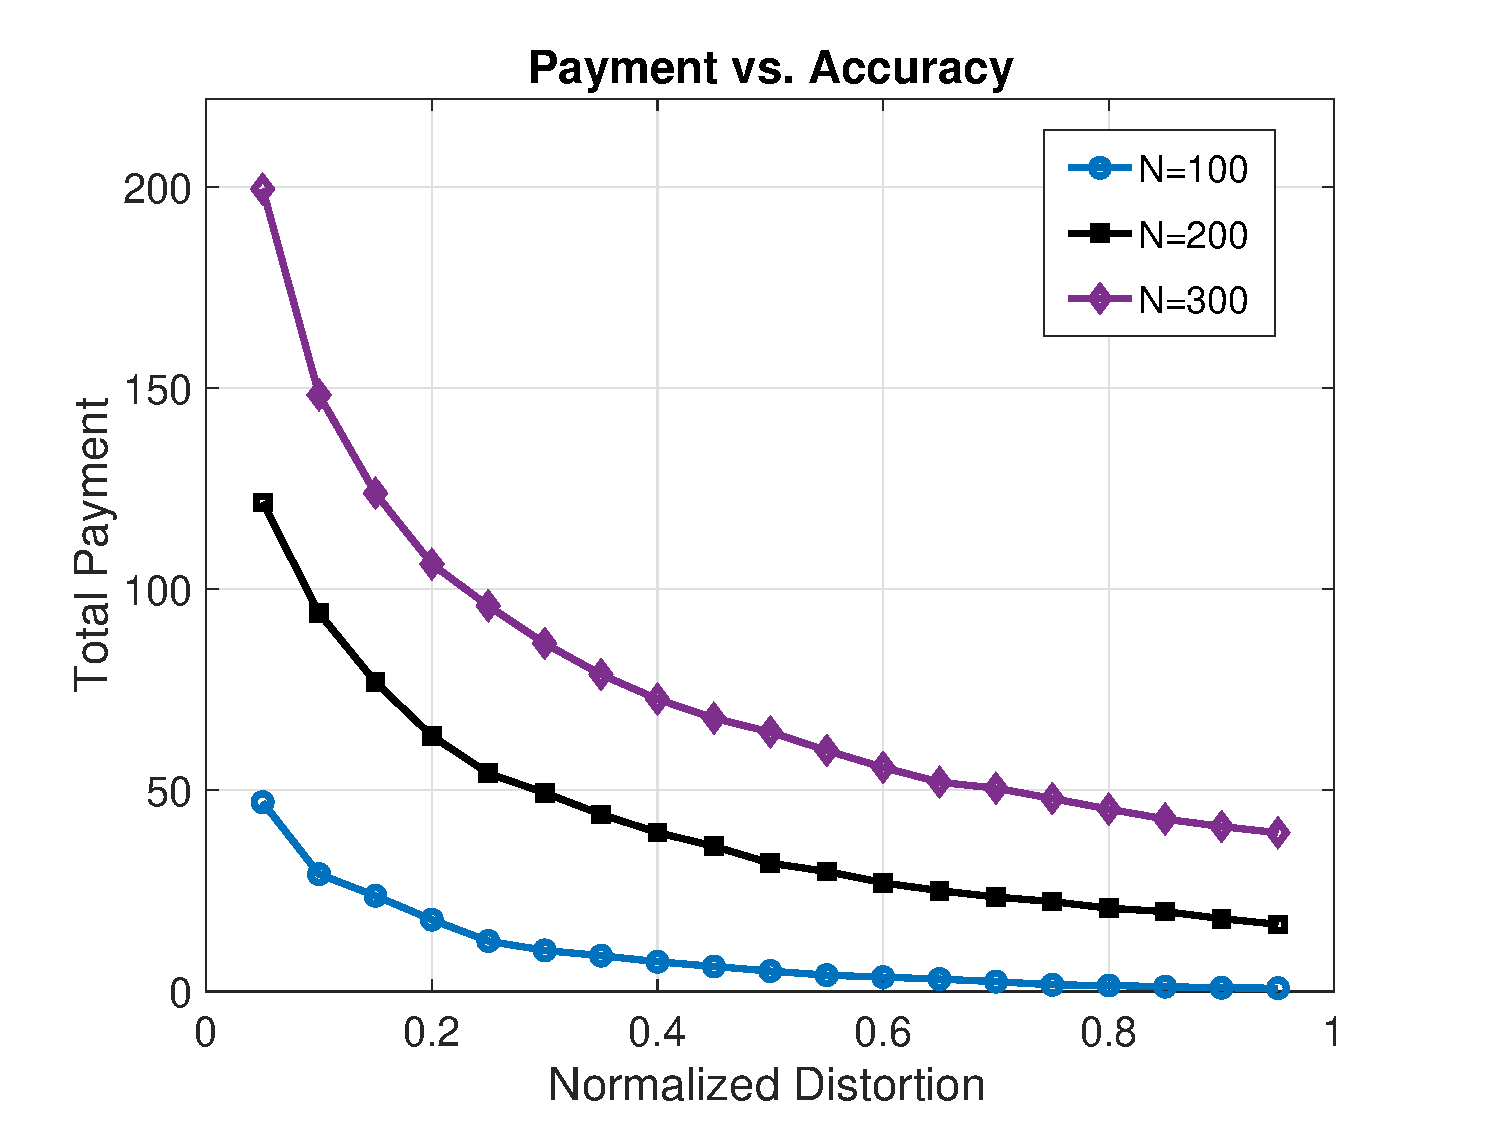
\includegraphics[scale=0.3]{./pic/payment_vs_accuracy5.eps}
%			%\caption{Payments under different accuracy requirements (privacy-passive case).}\label{fg:payment}
%			\caption{不同准确性约束下的平台支付(消极隐私保护情况)。}\label{fg:payment}
%		\end{minipage}
%		\hfill
%		\begin{minipage}[t]{0.48\textwidth}
%			\centering
%			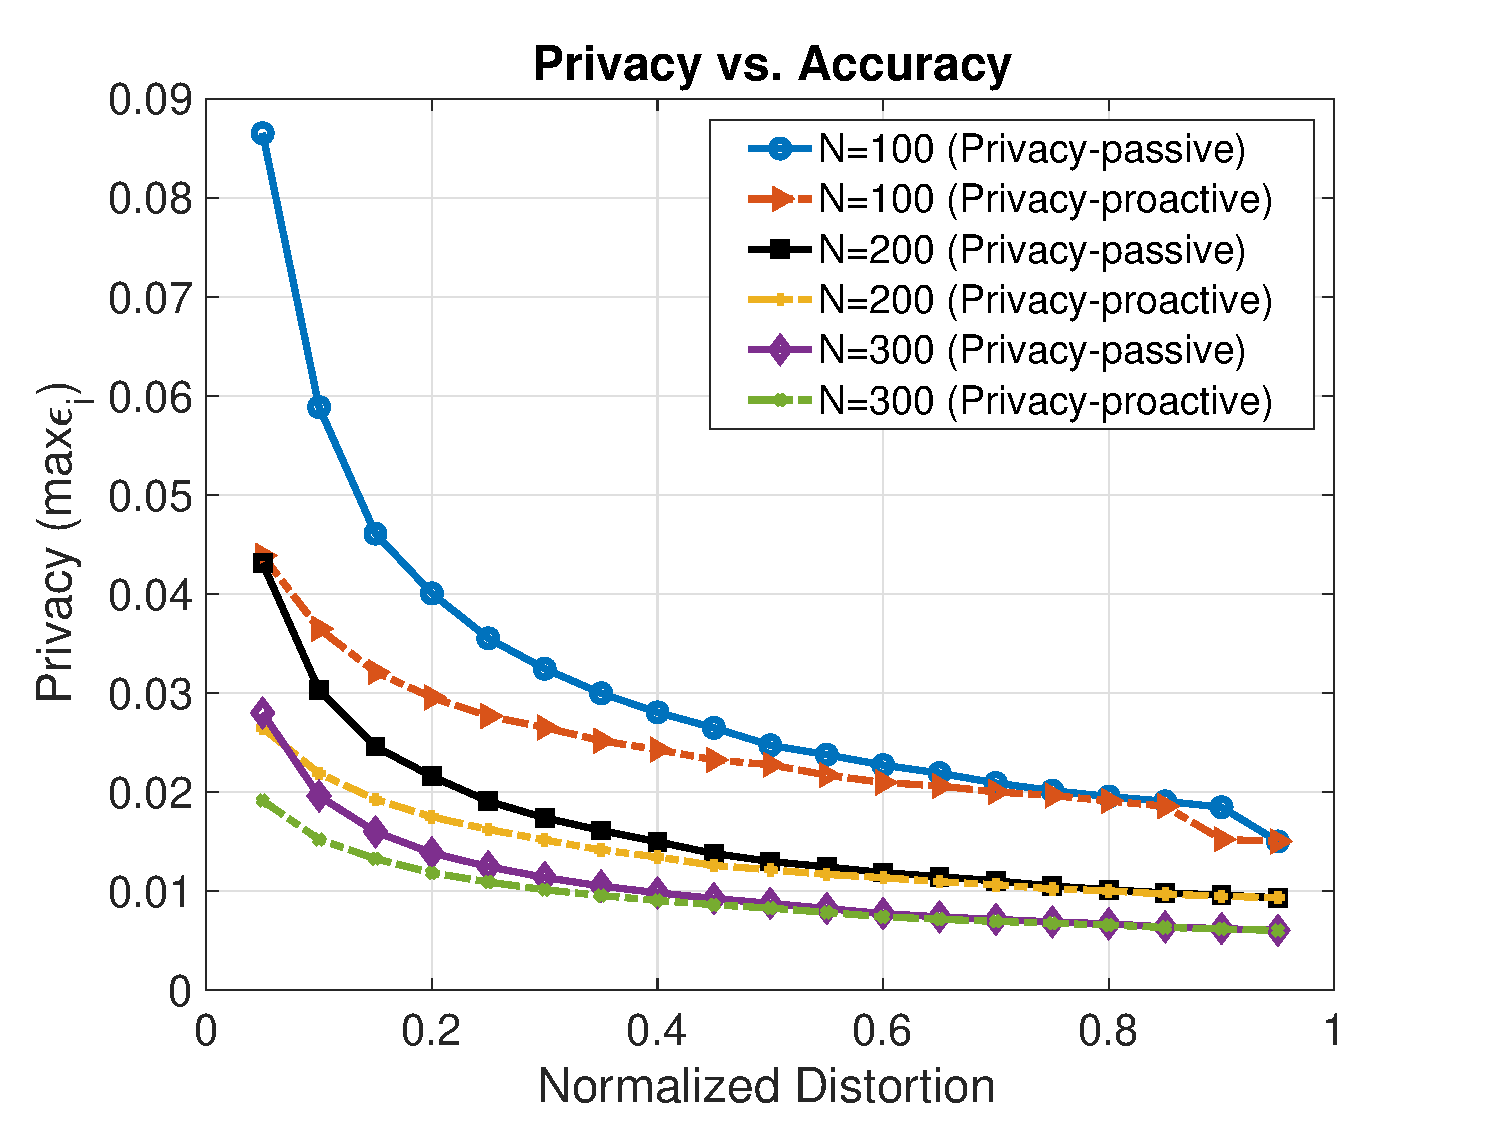
\includegraphics[scale=0.3]{./pic/privacy_vs_accuracy4.eps}
%			\caption{数据隐私与准确性之间的关系。}\label{fg:privacy}
%		\end{minipage}
%	\end{figure*}
	
	\begin{figure*}[!t]
%		\begin{minipage}[t]{0.48\textwidth}
			\centering
			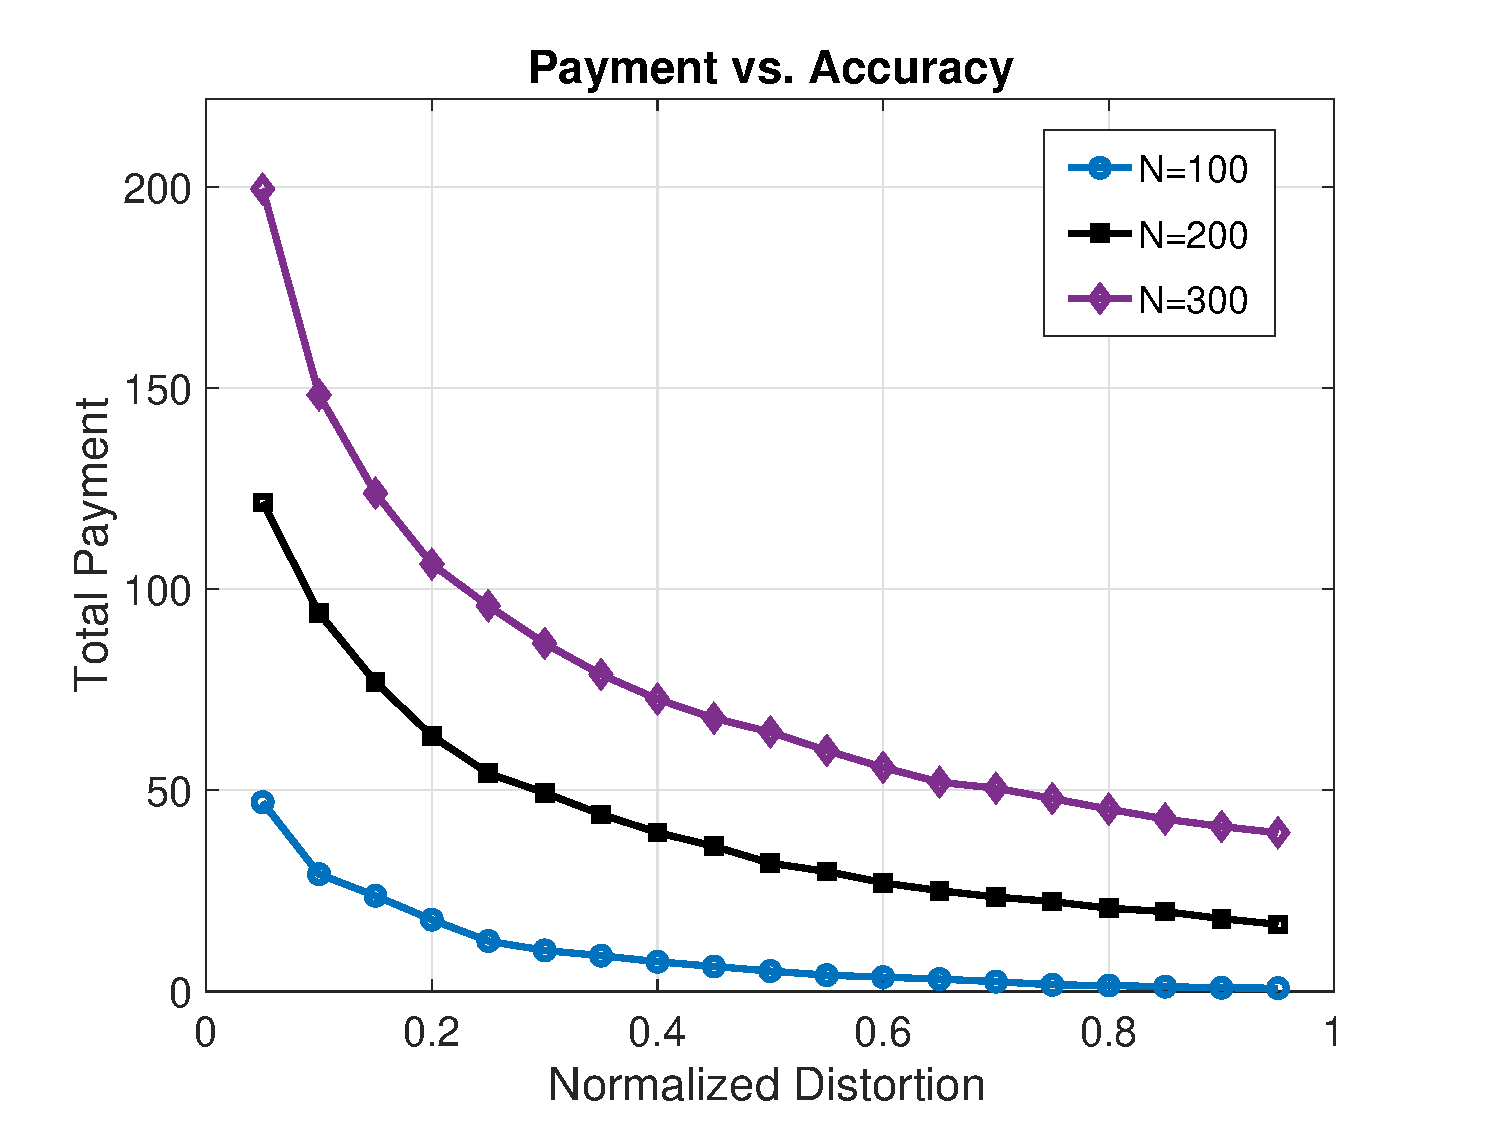
\includegraphics[scale=0.5]{./pic/payment_vs_accuracy5.eps}
			%\caption{Payments under different accuracy requirements (privacy-passive case).}\label{fg:payment}
			\caption{不同准确性约束下的平台支付(消极隐私保护情况)}\label{fg:payment}
	\end{figure*}
%		\end{minipage}
%		\hfill
%		\begin{minipage}[t]{0.48\textwidth}
	\begin{figure*}[!t]
			\centering
			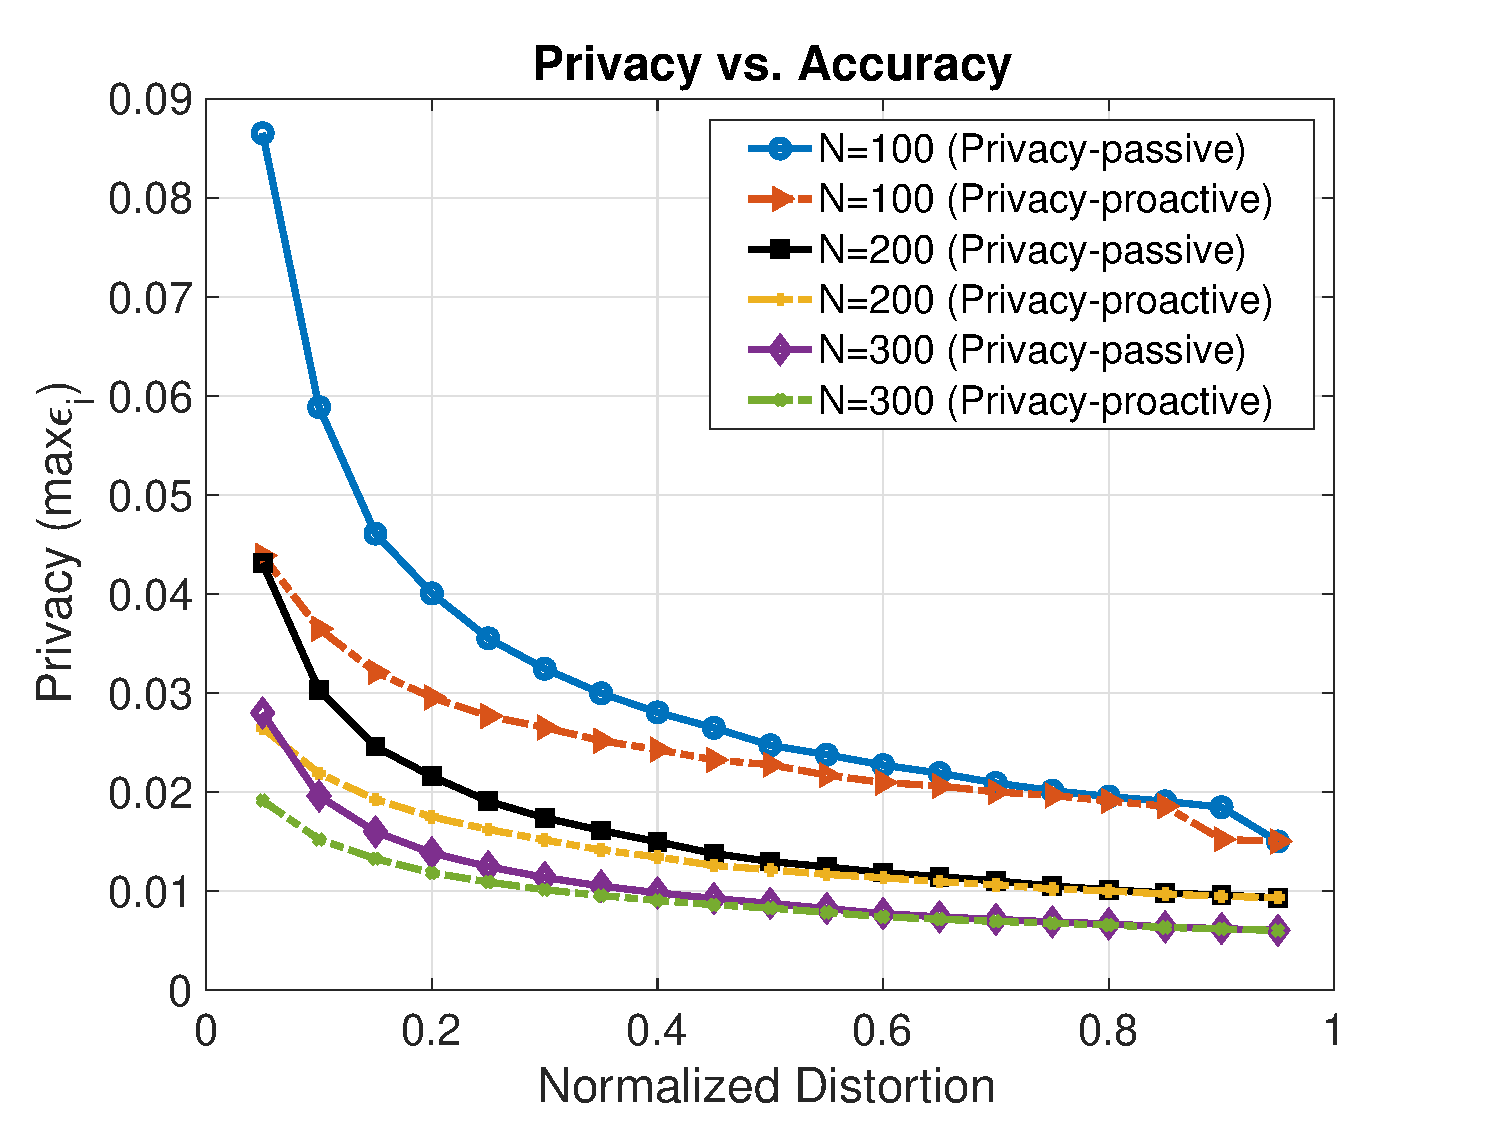
\includegraphics[scale=0.5]{./pic/privacy_vs_accuracy4.eps}
			\caption{数据隐私与准确性之间的关系}\label{fg:privacy}
%		\end{minipage}
	\end{figure*}	
	
	
	
	
	
%		\hfill
%		\begin{minipage}[t]{0.3\linewidth}
%			\centering
%			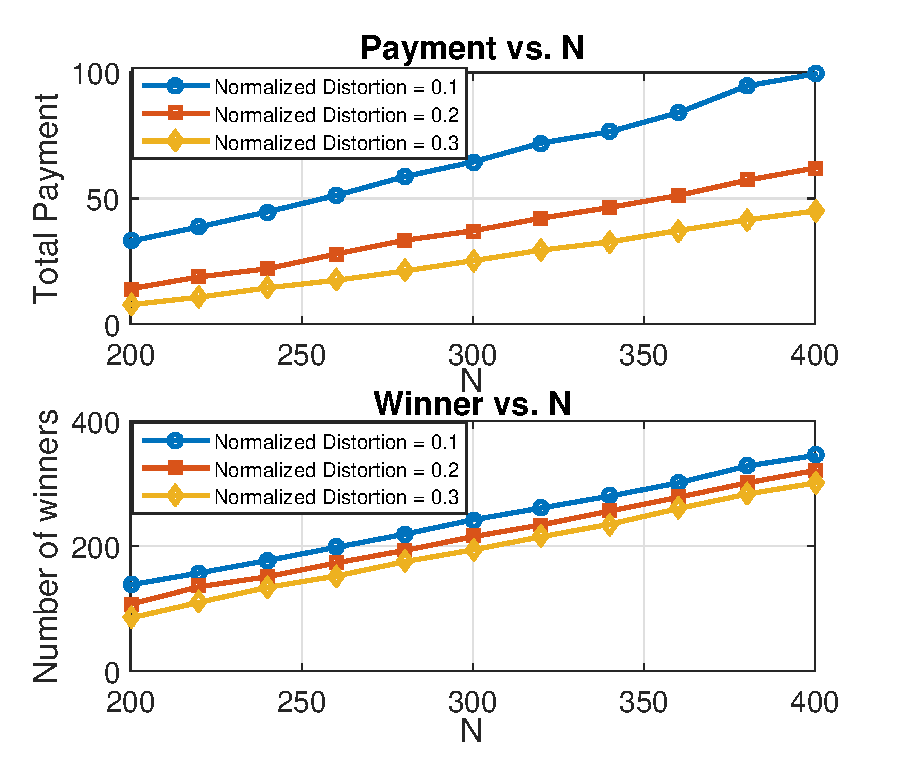
\includegraphics[scale=0.39]{./pic/externalities.eps}
%			\caption{Effect of externalities.}\label{fg:externalities}
%		\end{minipage}
		%\vspace{-0.5cm}
%		\vfill
%		\begin{minipage}[t]{0.48\textwidth}
%			\centering
%			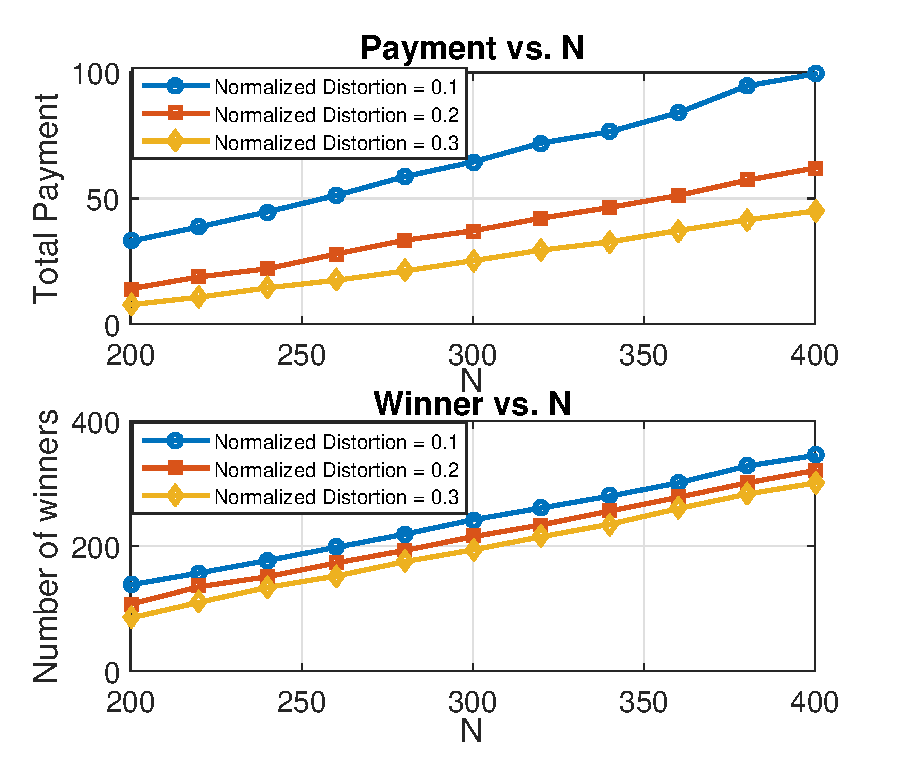
\includegraphics[scale=0.5]{./pic/externalities.eps}
%			\caption{Effect of externalities (privacy-passive case).}\label{fg:externalities1}
%		\end{minipage}
%	\begin{figure}
%		%\small
%		\subfigure[Privacy-passive case under different accuracy requirements.]{
%		\begin{minipage}[b]{0.45\textwidth}
%			\centering
%			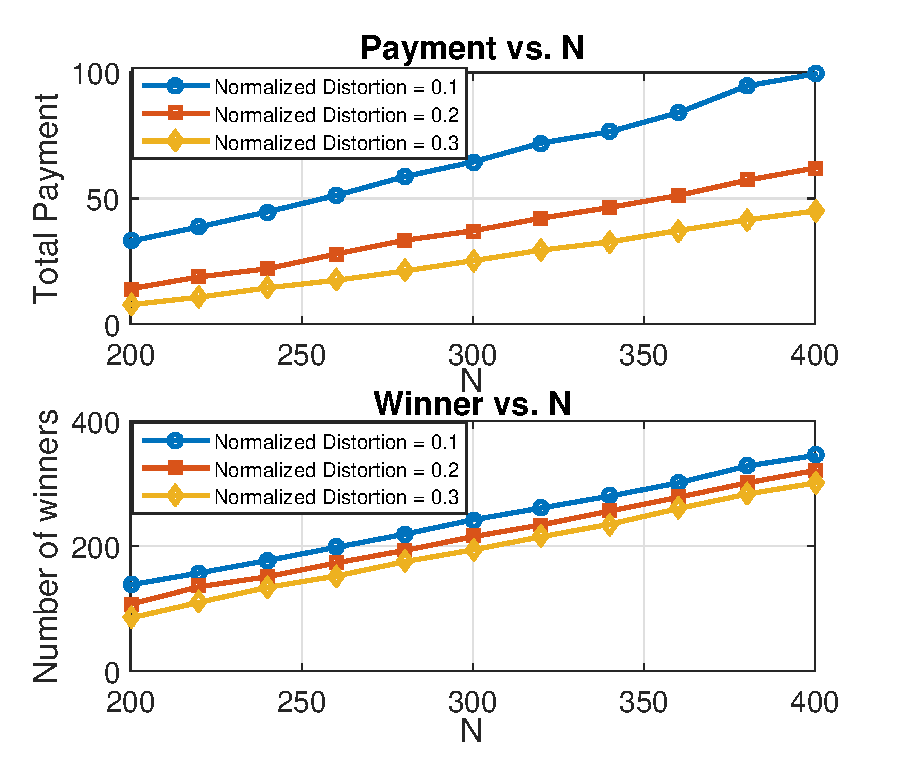
\includegraphics[scale=0.6]{./pic/externalities.eps}			
%		\end{minipage}}\label{fg:externalities1}
%		\subfigure[Comparison between privacy-passive case and privacy-proactive case (normalized distortion = 0.2).]{
%		\begin{minipage}[b]{0.45\textwidth}
%			\centering
%			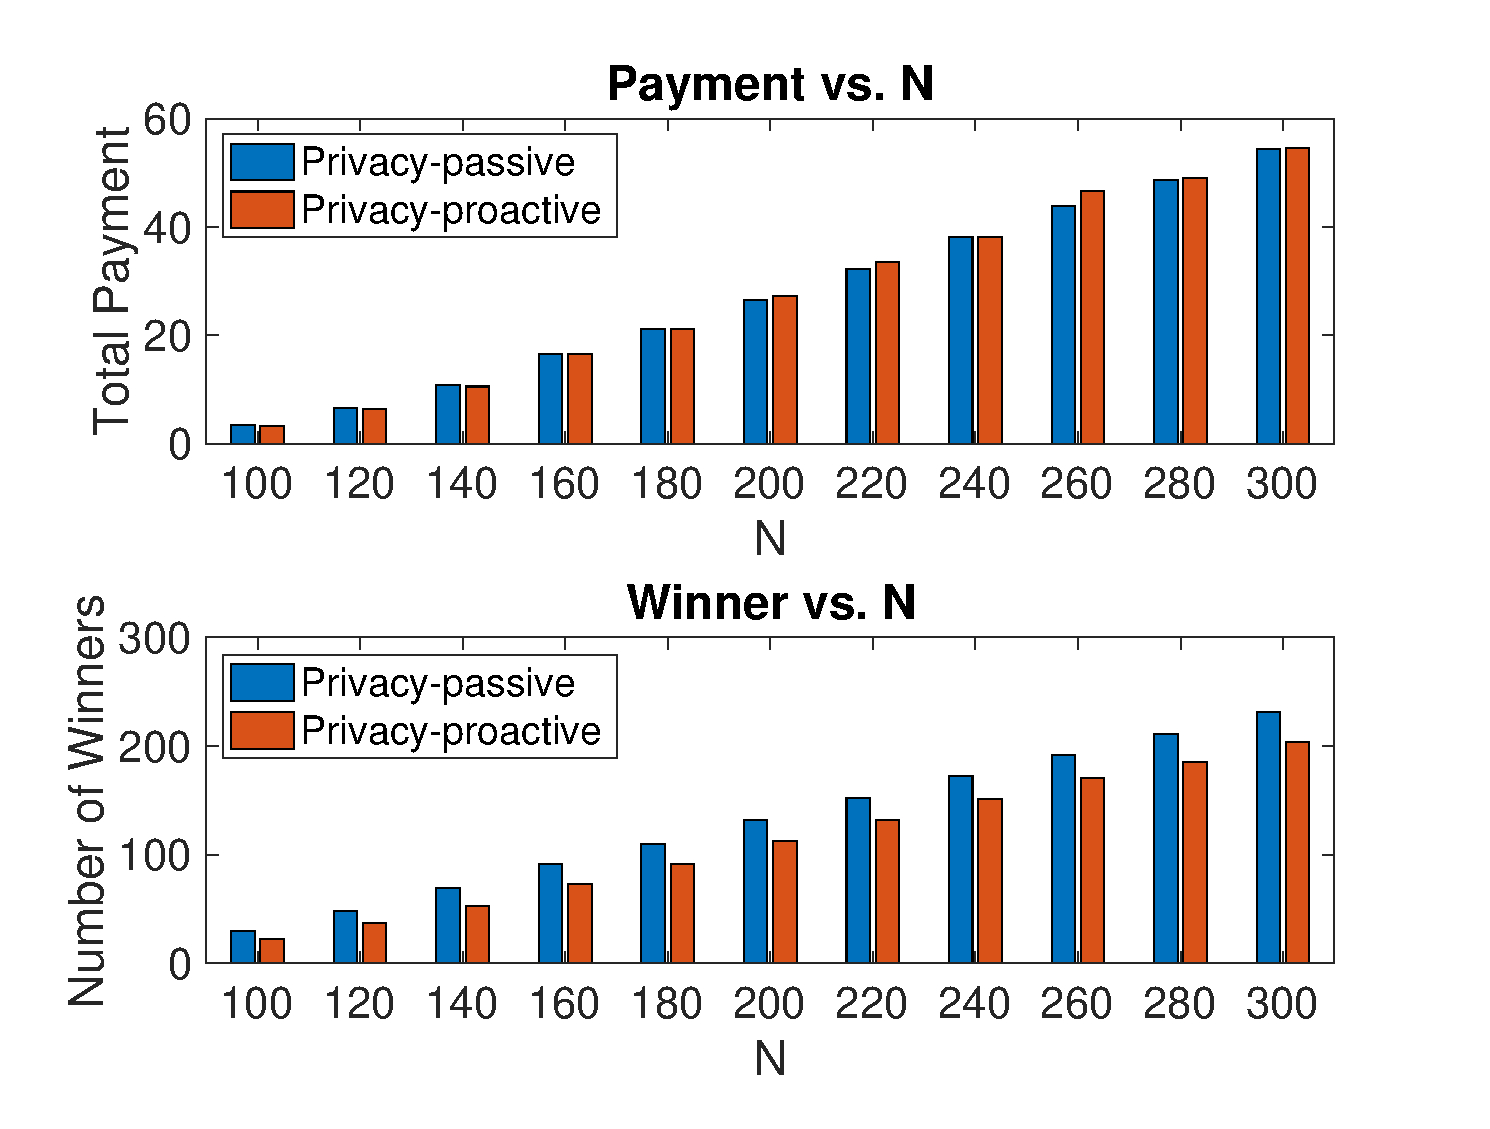
\includegraphics[scale=0.4]{./pic/externalities3.eps}
%		\end{minipage}}\label{fg:externalities2} %% label for second subfigure
%		\caption{Effect of externalities}
%		\label{fg:externalities}
%	\end{figure}
		
%	\begin{figure*}[!t]
%		\begin{minipage}[t]{0.48\textwidth}
%			\centering
%			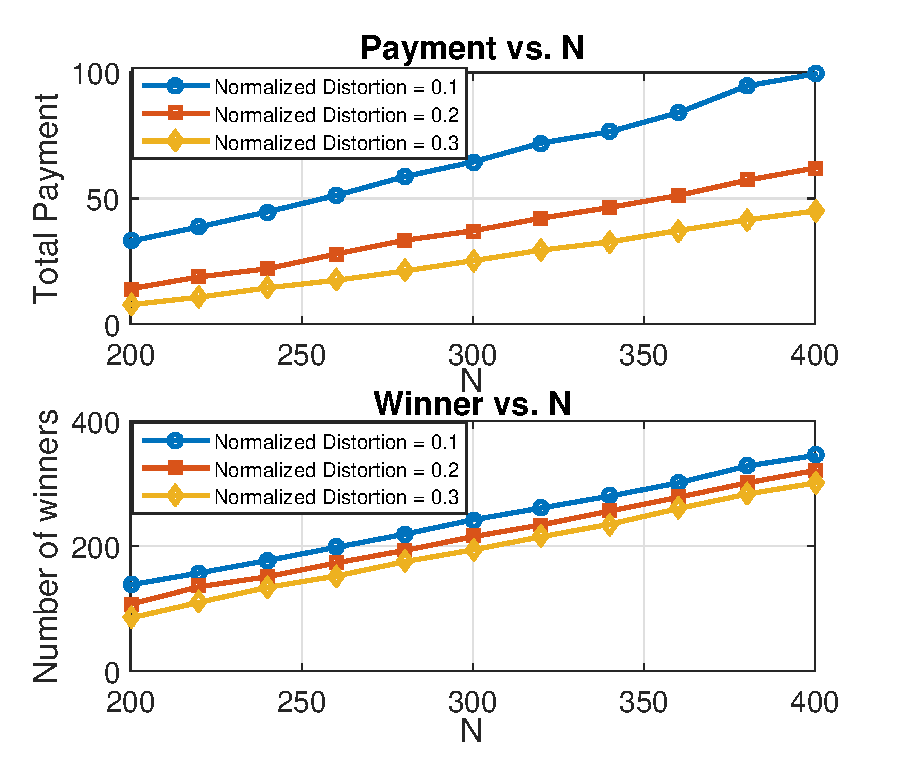
\includegraphics[scale=0.6]{./pic/externalities.eps}
%			\caption{不同准确性约束下用户总量的影响(消极隐私保护情况)。}\label{fg:externalities1}
%		\end{minipage}
%		\hfill
%		\begin{minipage}[t]{0.48\textwidth}
%			\centering
%			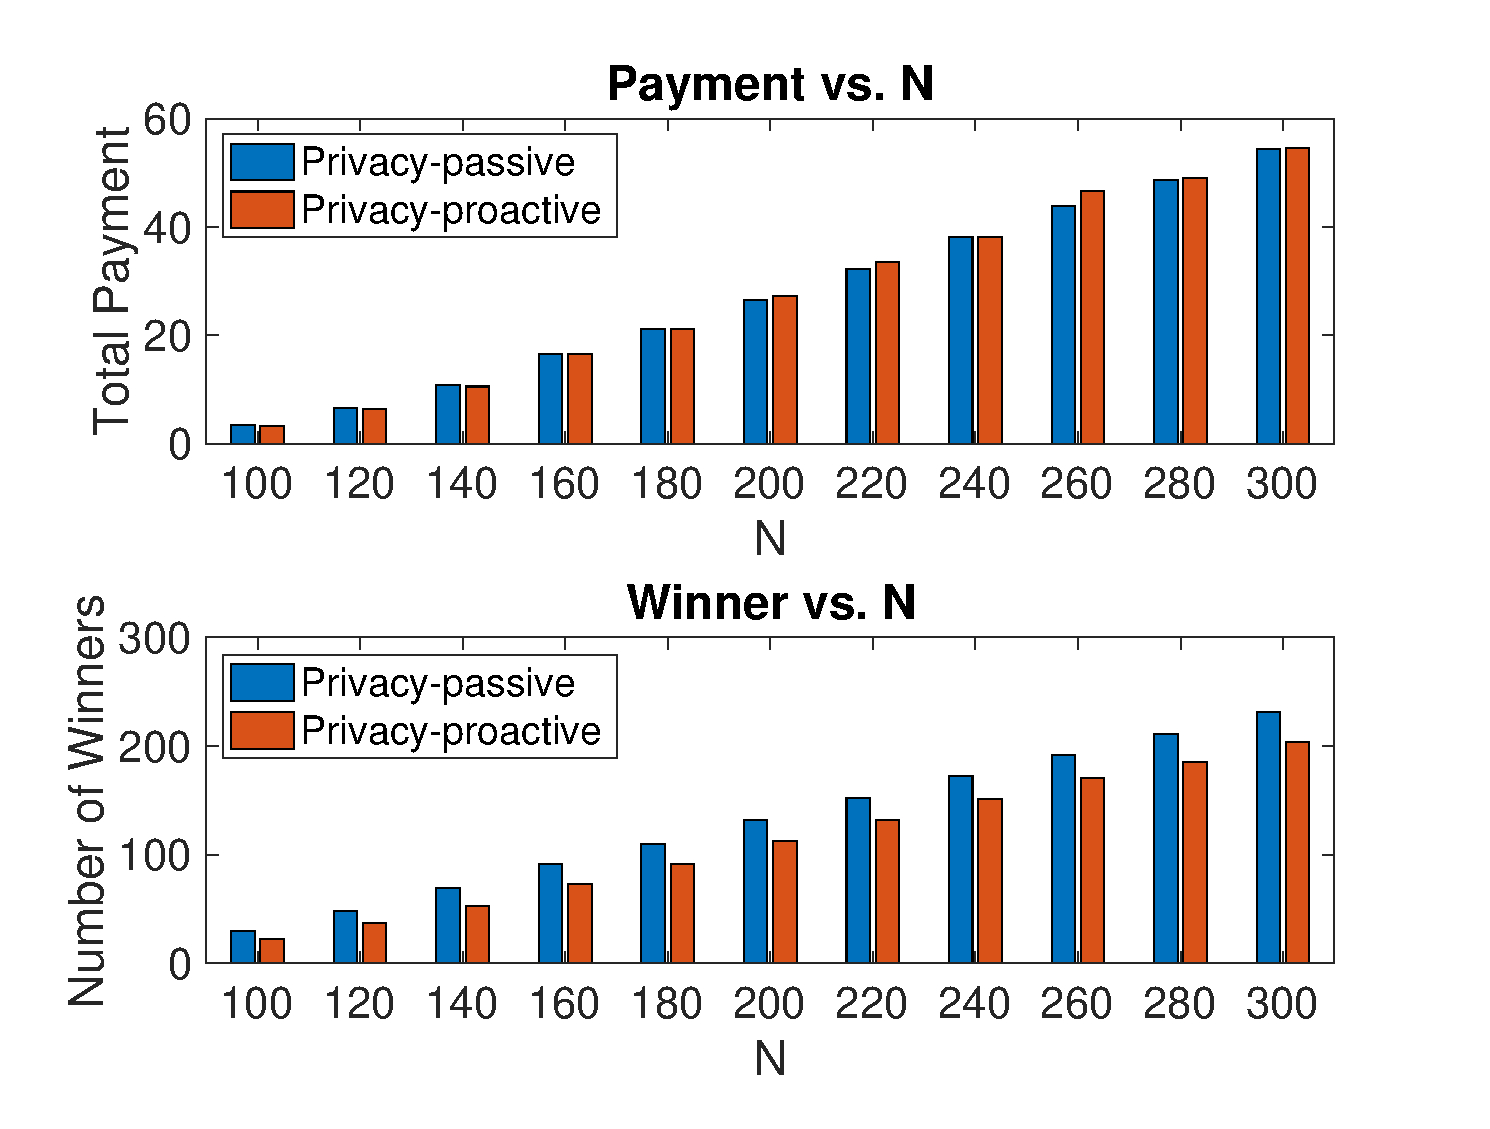
\includegraphics[scale=0.4]{./pic/externalities3.eps}
%			\caption{积极隐私保护与消极隐私保护之间的结果对比(归一化失真度要求 = 0.2)。}\label{fg:externalities2}
%		\end{minipage}
%		\caption{外部性影响}
%		\label{fg:externalities}
%	\end{figure*}		
	
	\begin{figure*}[!t]
%		\begin{minipage}[t]{0.48\textwidth}
			\centering
			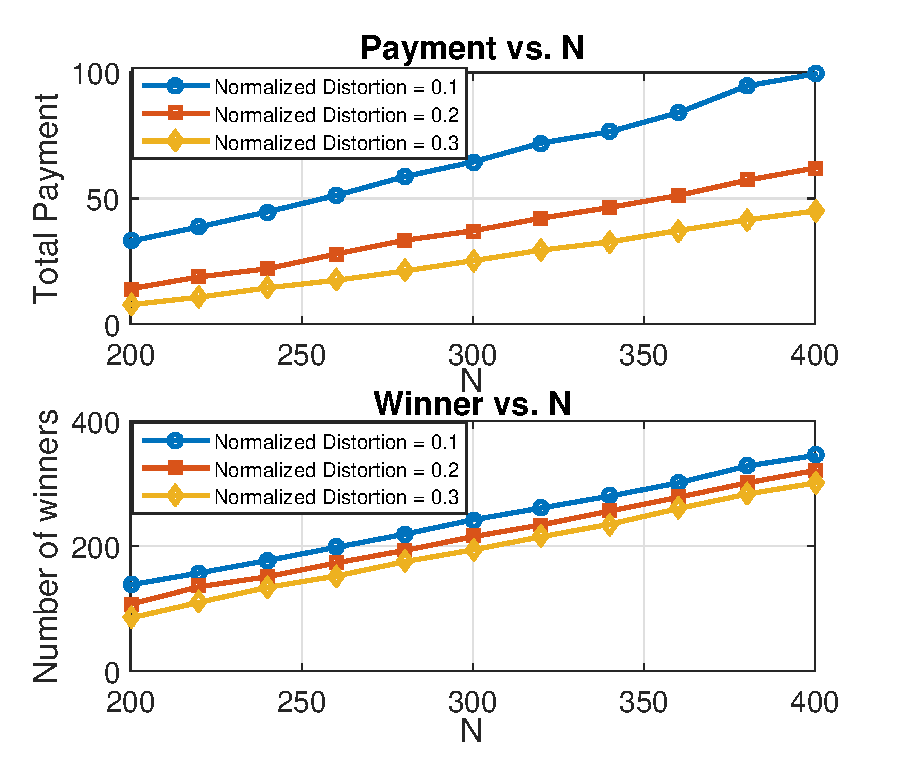
\includegraphics[scale=0.84]{./pic/externalities.eps}
			\caption{不同准确性约束下用户总量的影响(消极隐私保护情况)}\label{fg:externalities1}
%		\end{minipage}
%		\hfill
%		\begin{minipage}[t]{0.48\textwidth}
	\end{figure*}
	\begin{figure*}[!t]
			\centering
			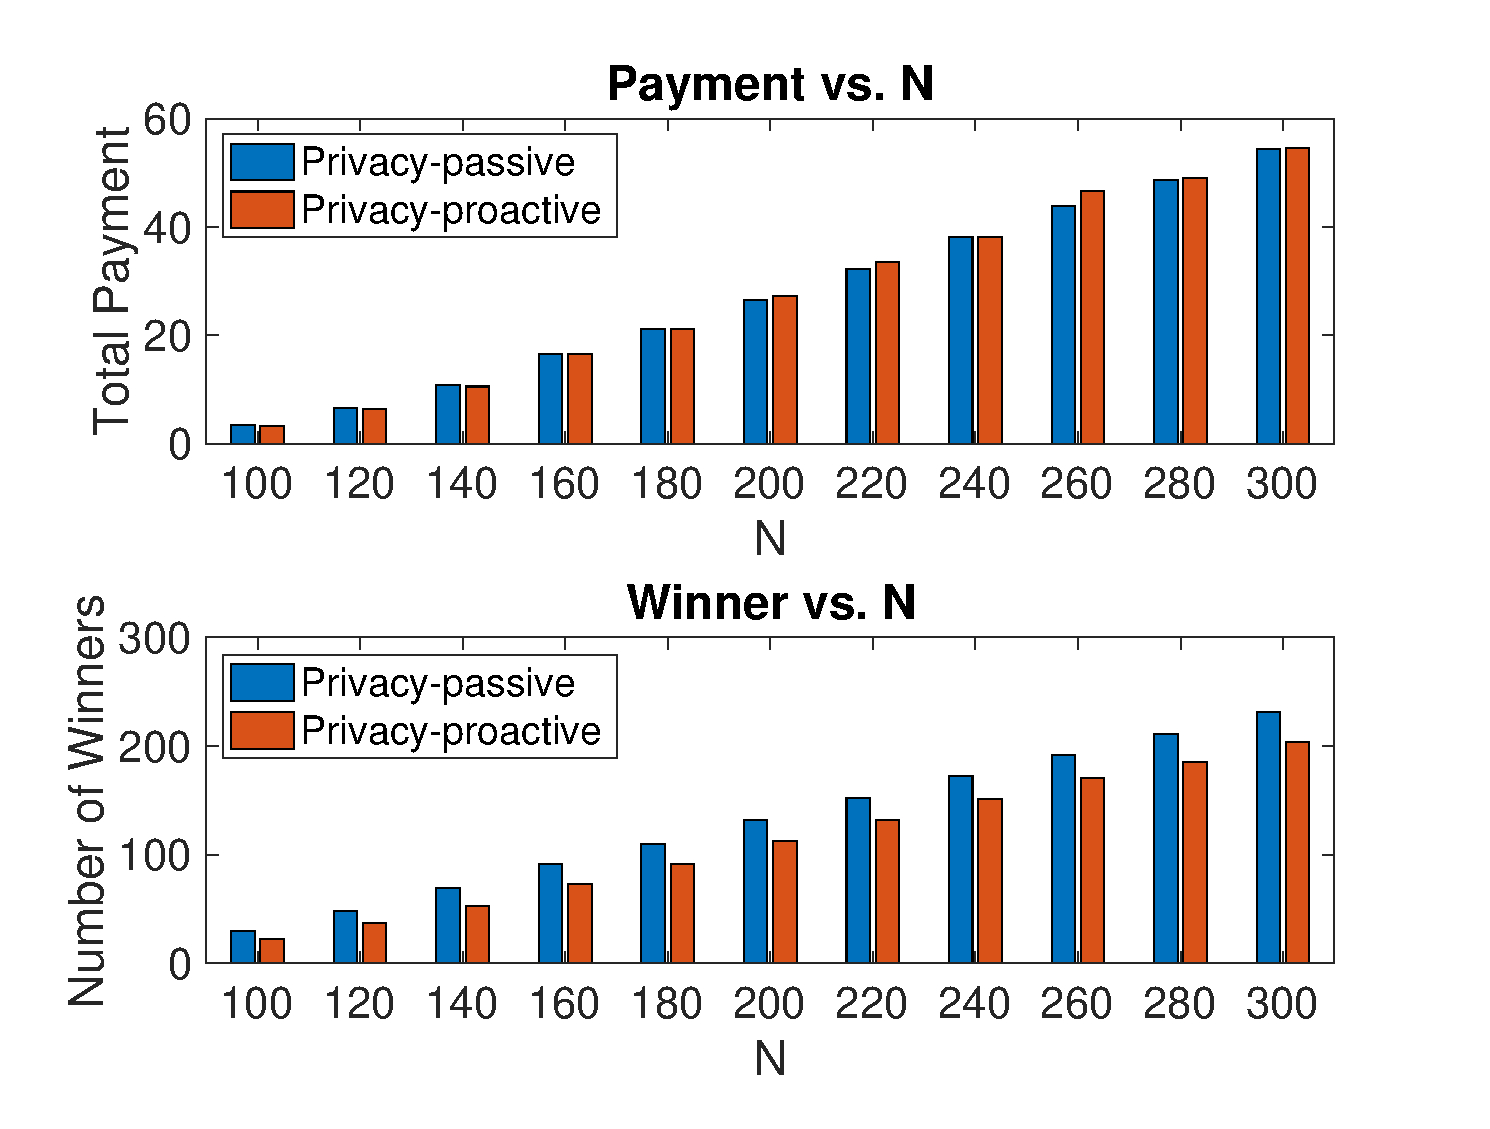
\includegraphics[scale=0.58]{./pic/externalities3.eps}
			\caption{积极隐私保护与消极隐私保护之间的结果对比(归一化失真度要求 = 0.2)}\label{fg:externalities2}
%		\end{minipage}
%		\caption{外部性影响}
%		\label{fg:externalities}
	\end{figure*}		
	
%		\centering
%		\subfloat[Privacy-passive case under different accuracy requirements.]{
%			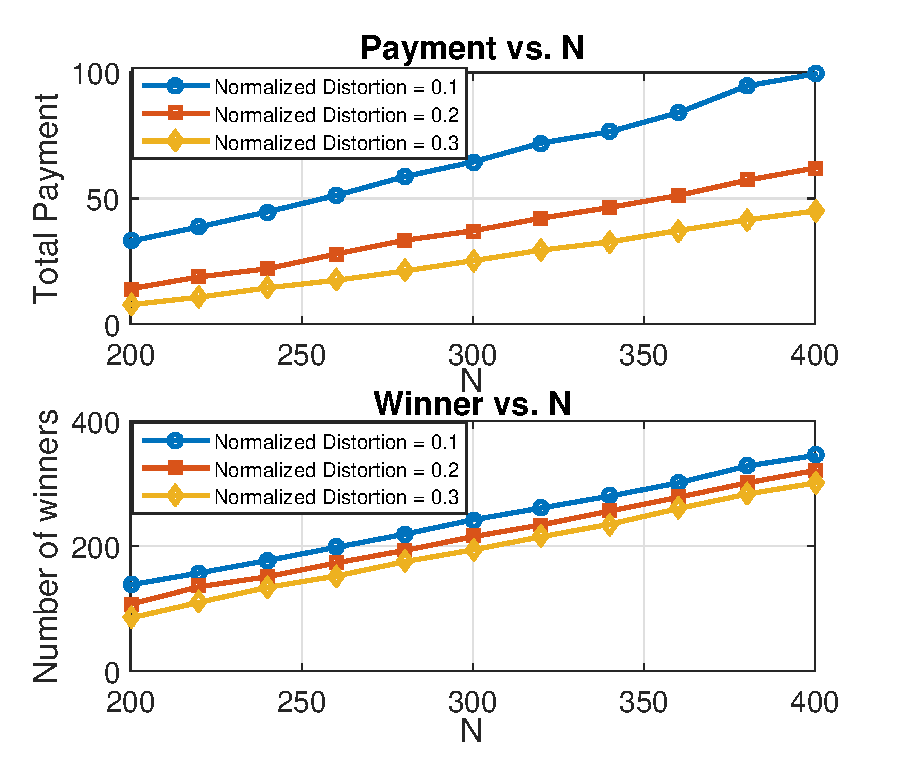
\includegraphics[scale=0.5]{./pic/externalities.eps}\label{fg:externalities1}}
%		%\hspace{0.45in}
%		\hfill
%		\centering
%		\subfloat[Comparison between privacy-passive case and privacy-proactive case (normalized distortion = 0.2).]{
%			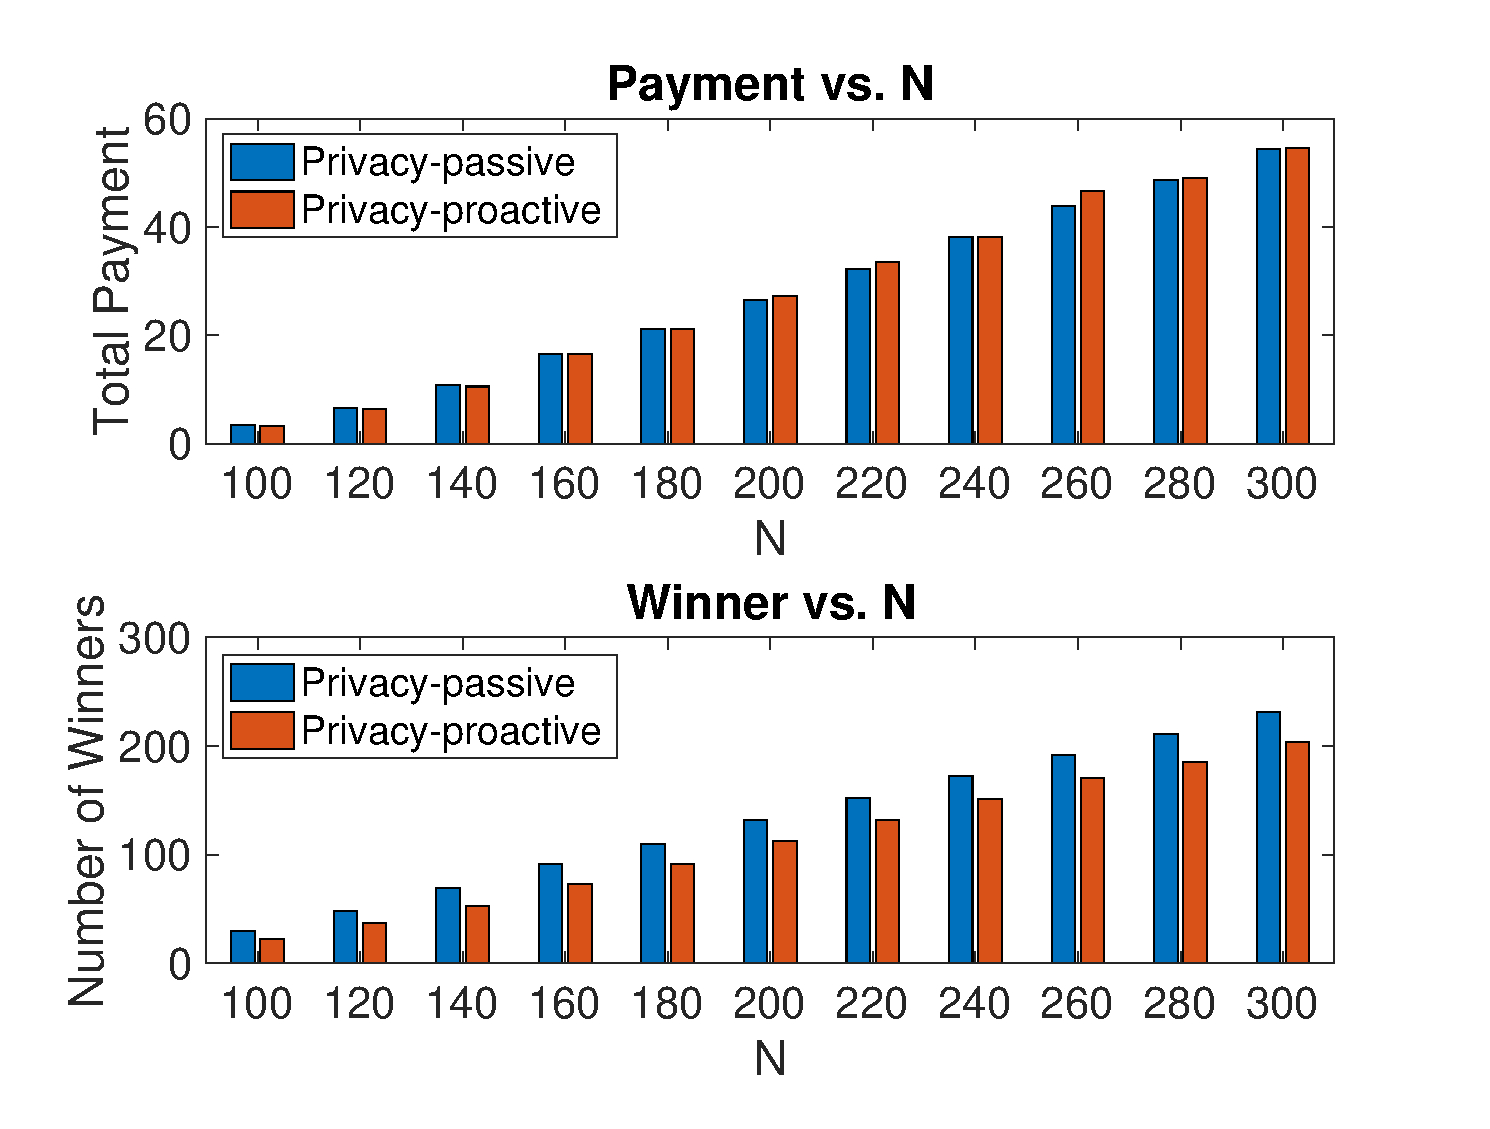
\includegraphics[scale=0.34]{./pic/externalities3.eps}\label{fg:externalities2}}
%		\hfill
%%		\begin{minipage}[t]{0.48\textwidth}
%%			\centering
%%			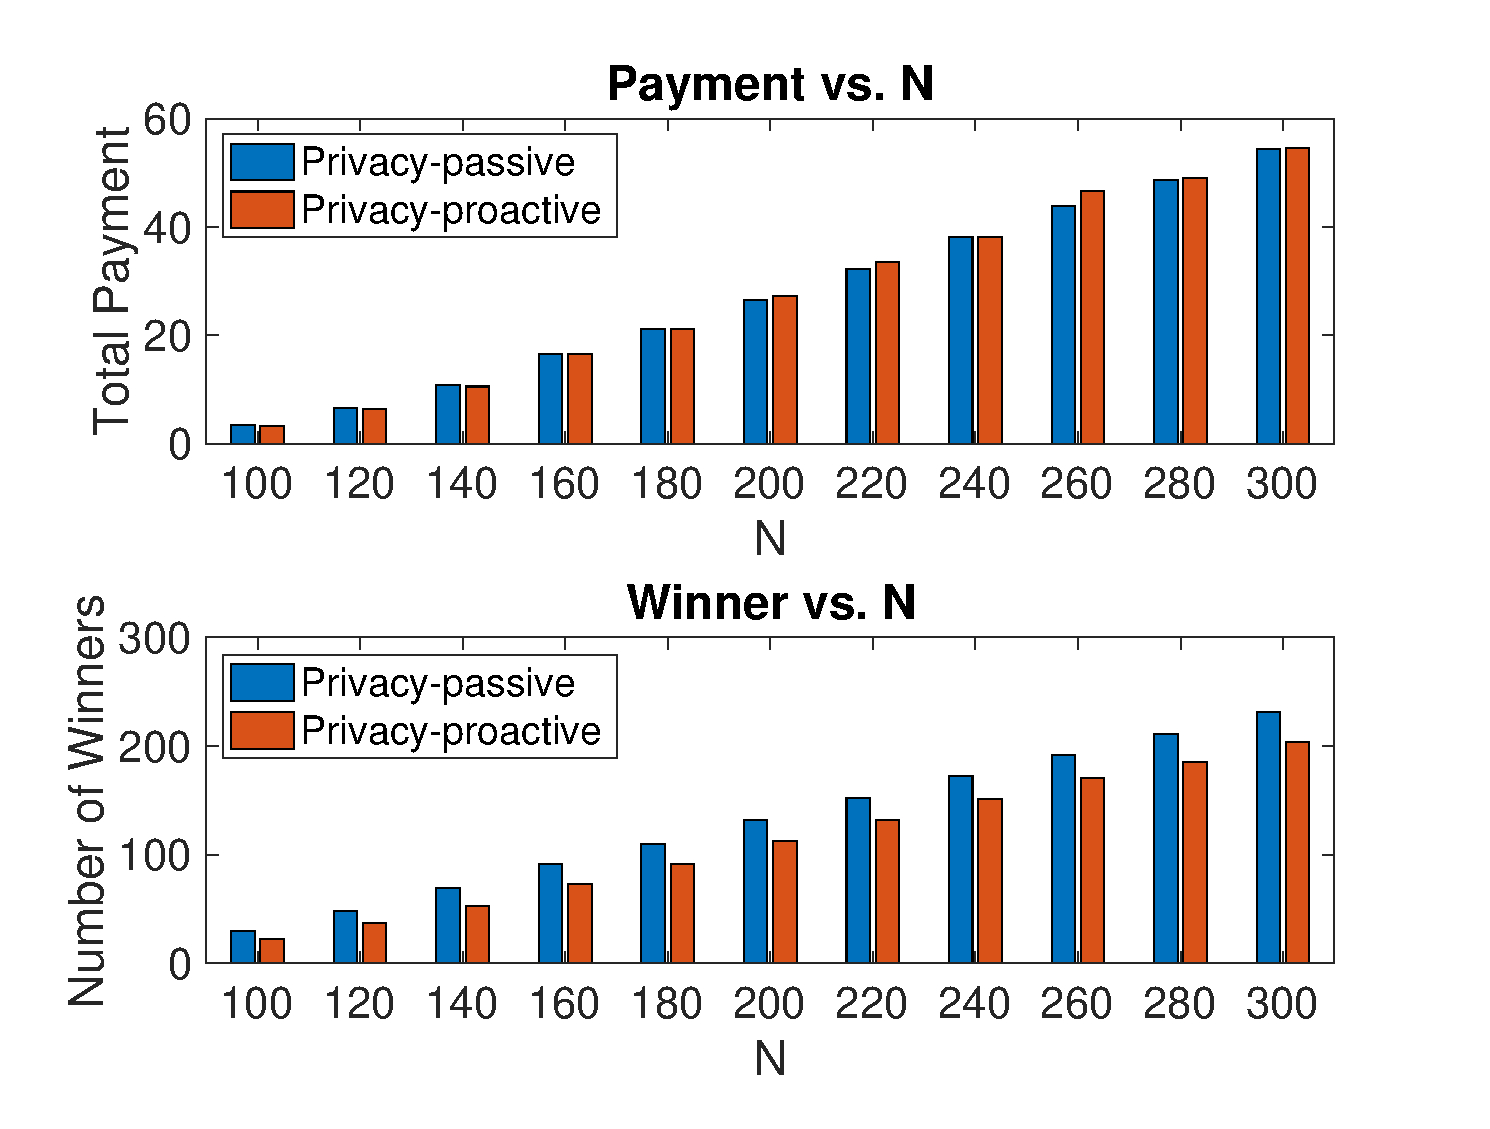
\includegraphics[scale=0.34]{./pic/externalities3.eps}
%%			\caption{Comparison between privacy-passive case and privacy-proactive case (normalized distortion = 0.2).}\label{fg:privacy}
%%		\end{minipage}
%		\caption{Effect of externalities}\label{fg:externalities}
		
		
		
%		\begin{minipage}[t]{0.3\linewidth}
%			\centering
%			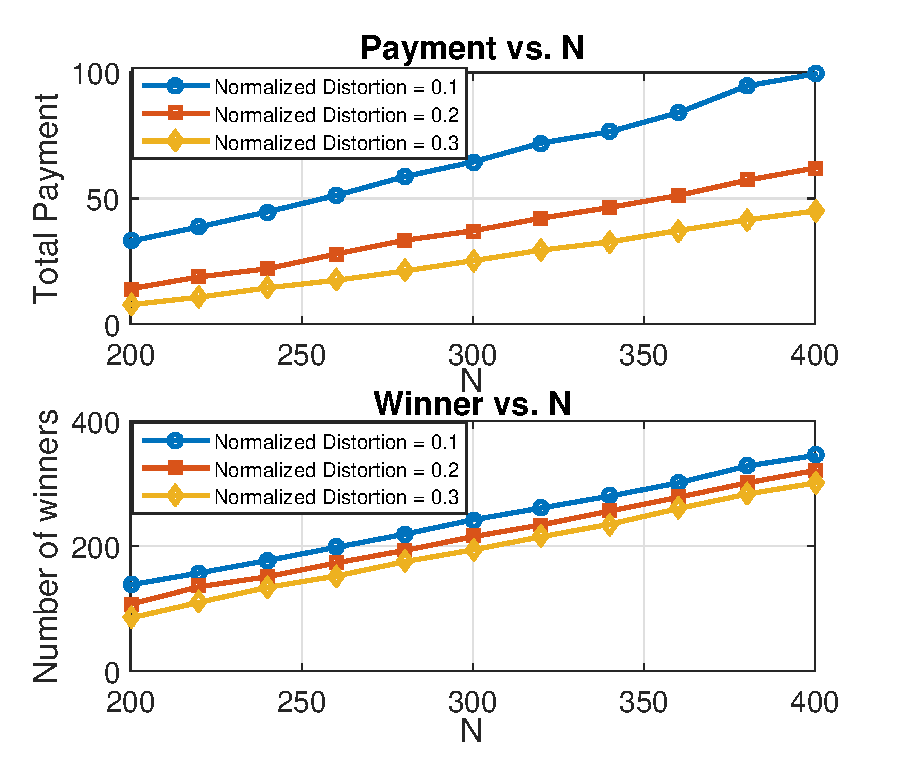
\includegraphics[scale=0.39]{./pic/externalities.eps}
%			\caption{Effect of externalities.}\label{fg:externalities}
%		\end{minipage}
%		\hfill
%		\begin{minipage}[t]{0.3\linewidth}
%			\centering
%			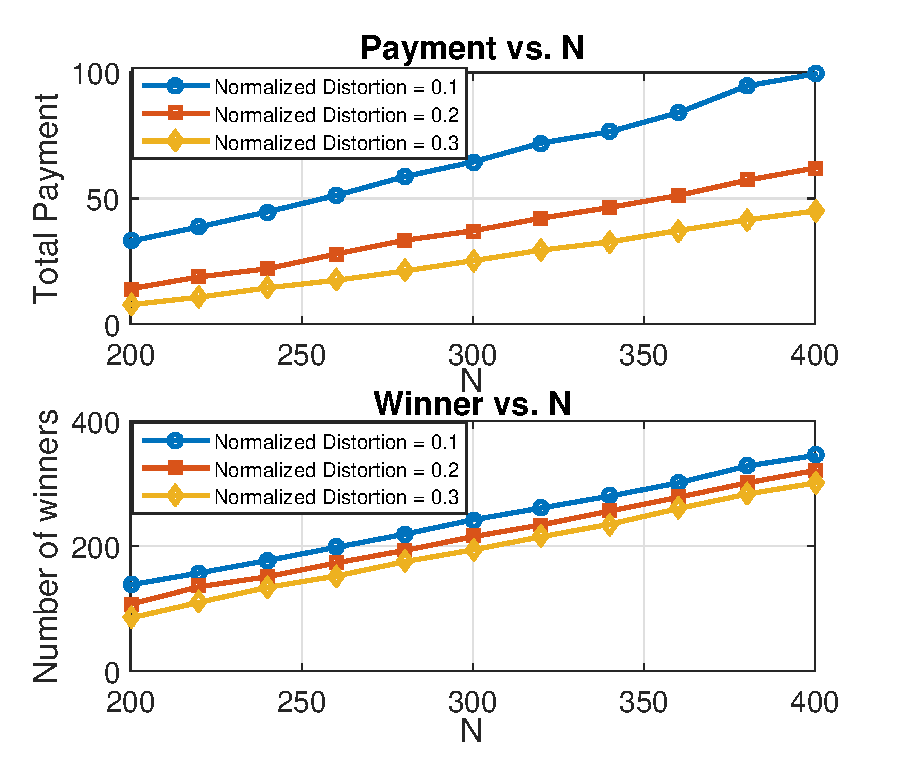
\includegraphics[scale=0.39]{./pic/externalities.eps}
%			\caption{Effect of externalities.}\label{fg:externalities}
%		\end{minipage}
	
%	\end{figure*}

\section{性能评估}\label{sec:pe}

\subsection{仿真设置}\label{sec:setup}
	在仿真中,我们随机生成用户的竞标价。具体的,我们从区间$[1, 20]$均匀地生成用户$i$的单位隐私成本$v_i$;对于积极隐私保护场景,我们从区间$[0.01, 0.2]$均匀地生成用户$i$的隐私保护级别固有要求$E_i$。我们从区间$[1,10]$均匀地随机生成每一个用户的权值,然后进行归一化处理。实验中的用户总数$N$的变化范围为100到300。失真度通过预设的最大失真度$\Delta_{\max}$进行归一化处理,保证$W$在不同失真度情况下总为正值。我们使用优化求解器CPLEX\cite{CPLEX}的二等分算法求解问题(\ref{eq:problem2})和问题(\ref{eq:problem1b})的最优解。由于据我们所知, 现有的群智感知激励机制研究工作尚未有考虑系统网络外部性的特征,因此在这里我们仅对DPDA算法和EDPDA算法进行评估实验。
	%In our simulation, we generate workers' bids at random. Specifically, the unit privacy costs are generated uniformly from the interval $[1, 20]$ and the data privacy level requirements are generated uniformly from the interval $[0.01, 0.2]$. The weights of workers are first generated uniformly at random from the interval $[1,10]$ and then normalized. The number of workers $N$ varies from 100 to 300. The distortion is normalized by some largest distortion $\Delta_{\max}$ such that $W$ is always positive under different distortions. The optimal solutions to the problem (\ref{eq:problem2}) and (\ref{eq:problem1b}) are calculated based on the bisection algorithm using the CPLEX optimization solver \cite{CPLEX}. To the best of our knowledge, as there are no auction mechanisms for mobile crowdsensing allowing workers to report noisy data while considering the externalities, we examine only the performance of the DPDA algorithm and the EDPDA algorithm we proposed in this paper.
	
	\vspace{-0.2cm}
	\subsection{结果和讨论}
	
	%\noindent{\textbf{Payment versus Accuracy.}}
	\noindent{\textbf{奖励 vs. 准确性}}
	在图\ref{fg:payment}中,我们展现了平台总支付在不同结果准确性约束下的变化趋势。我们观察到,随着准确性约束放宽(归一化失真度要求变大),平台总支付会单调降低。其背后原因是$W$会随着$\Delta$数值的增加而减少,即准确性要求放宽后平台不需要在“购买”较准确的用户隐私数据上产生过多成本。同时,我们发现对于相同水平的失真度要求,平台的总支付额随着用户总数的增加而增加。这是由于对于相同水平的失真,$W$随着用户数量的增加而增加(\ref{eq:problem2}),使得平台必须征召更多的用户,从而导致总付款额的增加。
	%In Fig. \ref{fg:payment}, we illustrate the payments under different accuracy requirements with different total number of privacy-passive workers. We observe that as the distortion level increases, the total payments decrease, simply because $W$ decreases as $\Delta$ increases, i.e., the platform does not need to purchase much privacy from workers. Meanwhile, for the same level of distortion, the total payments increase with the number of workers, because $W$ increases with the number of workers for the same level of distortion based on (\ref{eq:problem2}), which requires the platform to select more workers and thereby the total payments increase. 
	
	%\begin{figure}[h!]
	%	\centering
	%	\includegraphics[scale=0.4]{./pic/payment_vs_accuracy1.eps}
	%	\caption{Payments under different accuracy requirements with different total number of workers.}\label{fg:payment}
	%\end{figure}
	
	\noindent{\textbf{隐私 vs. 准确性}}
	在图\ref{fg:privacy}中,我们阐明了数据隐私保护级别与结果准确性约束之间的关系。我们使用所有参与用户中最低的隐私保护级别(即$\epsilon=\max_{i\in\mathcal{S}}\epsilon_i$)来表示某一准确性约束(失真度要求)的系统隐私保护级别。正如我们所预期的,随着准确性约束放宽,数据隐私保护级别会有所升高(即$\epsilon$越小,隐私保护级别越高),与节\ref{sec:pvsa}中的分析相符合。实验结果同时清除地表明积极隐私保护场景下的用户普遍会比消极隐私保护场景下的用户得到更高的隐私保护级别,而这正是由于积极隐私保护场景下的用户会对其隐私保护级别有固有的要求。
	%In Fig. \ref{fg:privacy}, we illustrate the relationship between the data privacy and the accuracy. As the privacy of each worker is different, we use the maximum of all the workers' $\epsilon_i$  ($\epsilon=\max_{i\in\mathcal{S}}\epsilon_i$) to denote the privacy protection level at the given distortion level. As expected, as the distortion level increases,  the data privacy level increases (the smaller $\epsilon$, the higher the privacy protection level), which agrees with our analysis in Section \ref{sec:pvsa}. The results clearly show that privacy-proactive workers in general experience higher privacy level than the privacy-passive workers, which agrees with our expectation since privacy-proactive workers have imposed customized privacy level requirement once enter into the crowdsensing system. 
	
	%\begin{figure}[h!]
	%	\centering
	%	\includegraphics[scale=0.4]{./pic/privacy_vs_accuracy2.eps}
	%	\caption{Relationship between data privacy and the accuracy.}\label{fg:privacy}
	%\end{figure}
	
	\noindent{\textbf{单重负网络外部性}}
	在图\ref{fg:externalities1}和图\ref{fg:externalities2}中,我们阐明了单重负网络外部性的影响。如同节\ref{sec:formulation}中所讨论的,每个用户的数据隐私保护级别取决于其他用户的参与。当参与用户的数量改变时,用户们的隐私保护级别也相应发生变化。当用户数量增加时,平台需要征召的用户数量也随即增加以维持相同的结果准确性。因此,我们可以从实验结果中观察到当用户总数增加时,平台的总支付和参与的用户数量都有相应的增加。图\ref{fg:externalities1}则清除地说明了准确性要求越低(失真度水平越高),平台总支付和参与的用户数量约少。
	%Fig. \ref{fg:externalities} illustrates the effect of externalities. As discussed in Section \ref{sec:formulation}, the data privacy level of each worker depends on other workers' participations, and when the  number of workers changes, it would change workers' privacy levels. As the number of workers increases, the platform needs to hire more workers to maintain the same distortion level. Therefore, we can observe that the increase of total payments and the number of winners as the worker set enlarges. Fig. \ref{fg:externalities1} clearly shows that the higher the distortion level, the lower the total payment and the less the number of winners. 
	在图\ref{fg:externalities2}中,我们进行了隐私消极保护场景和因司机及保护场景的对比。可以看到,在给定归一化失真度和用户集大小的情况下,两种场景下平台所需支付的总付款额几乎相同。这是由于积极隐私保护场景下参数$W$并不受用户$i\in\N$的固有隐私级别要求$g_i$的影响。此外,我们观察到,积极隐私保护场景下的拍卖获胜者人数通常少于消极隐私保护场景下的获胜者人数。这是因为对隐私保护级别的固有要求使少数用户失去了参与感知任务的条件,直接导致了用户人数的减少。因而在单重负外部性的影响下,获胜者的数量减少了。
	%In Fig. \ref{fg:externalities2}, we show the comparison results of the privacy-passive case and privacy-proactive case. We can see that almost the same total payment has to be consumed in the two cases given a fixed normalization distortion with a fixed size of worker set, as $W$ is not influenced by the imposed privacy level requirement $g_i$ of each worker $i\in\N$. Moreover, we observe that the number of winners in the privacy-proactive case is in general less than the number of winners in the privacy-passive case. This is because the additional requirement on privacy level renders a few workers unqualified for being evolved into the private crowdsensing, which leads to the shrink of worker set. Under the effect of externality, the number of winners decreases.

	
	%\begin{figure}[h!]
	%	\centering
	%	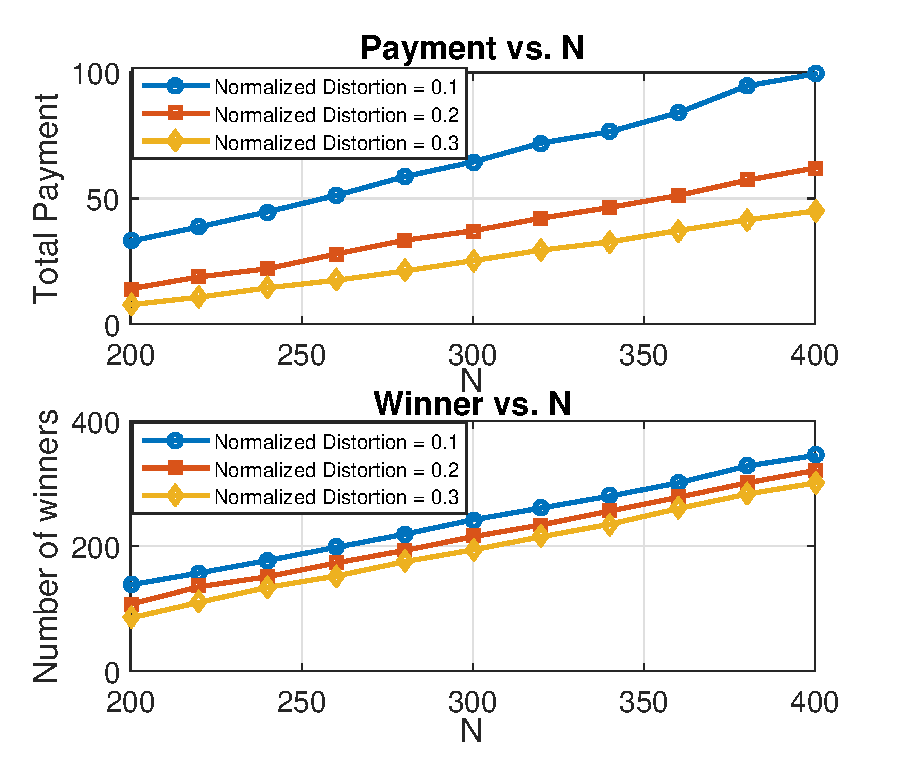
\includegraphics[scale=0.4]{./pic/externalities.eps}
	%	\caption{Effect of externalities.}\label{fg:externalities}
	%\end{figure}
	
	
	\noindent{\textbf{算法近似度}}
	在表\ref{tab:optimality}中,我们通过分别比较DPDA算法和EDPDA算法输出结果与相应最优值的差异来说明两个算法的性能。对于每个$N$的取值,我们运行100次实验,并且在每个实验中,我们都会随机生成节\ref{sec:setup}中提到的参数。
	%In Table \ref{tab:optimality}, we illustrate the performance of the proposed DPDA algorithm and EDPDA algorithm respectively by comparing their output total payment with the optimal ones. For each $N$, we run 100 experiments and in each experiment, we randomly generate the parameters as mentioned in Section \ref{sec:setup}. 
	在不同的实验设置下,我们观察到两种算法得到的总付款都非常接近最优值,两个算法的最大近似比约为2。
	%Under different settings, we observe that the total payments generated by these two algorithms are very close to the optimal one and the maximal approximation ratio for each case is around 2. 
	相比之下,DPDA算法的近似率优于EDPDA。这是因为在积极隐私保护的场景下,平台除了要考虑成本最小化的目标外,还须考虑用户的固有隐私保护级别要求。
	%EDP​​DA算法的拍卖获胜者选择过程通过先筛选出满足隐私保护级别要求的工人,然后选择优化付款的获胜者,而不是在选择获胜者时共同考虑这两个因素,从而将这两个因素解耦。
	%By comparison, DPDA algorithm outperforms EDPDA in terms of the approximation ratio. This is because that in the privacy-proactive scenario, the platform has to take into account workers' privacy level requirements in addition to the objective of payment minimization. And the winner determination procedure of EDPDA algorithm decouples the two factors by first filtering out workers whose privacy level requirements are satisfied, then selecting out winners that optimize the payment, instead of jointly considering both two factors while choosing the winners.
	
%	\begin{table}[h!]
%			\vspace{-0.3cm}
%		\caption{Approximation ratio of the DPDA algorithm, where we choose the normalized distortion equal to 0.2.}
%		\vspace{-0.2cm}
%		\label{tab:optimality}
%		\centering \tabcolsep 5pt
%		\begin{tabular}{|c|c|c|c|}
%			\hline
%			Number of workers $N$  & 200 & 300 & 400 \\
%			\hline
%			Average approximation ratio   & 1.88 &1.85& 1.85\\
%			\hline
%			Minimal approximation ratio   & 1.71 &1.69& 1.70\\
%			\hline
%			Maximal approximation ratio   &  2.15    & 2.07   & 1.99      \\
%			\hline
%		\end{tabular}
%
%	\end{table}

	\begin{table}[h!]
%			\vspace{-0.3cm}
		\caption{DPDA和EDPDA算法的近似率(归一化失真度要求 = 0.2).}\label{tab:optimality}
		%\vspace{-0.3cm}
		
		\centering \tabcolsep 5pt
%		\subfloat[DPDA Algorithm]{
		\subfigure[DPDA算法]{
		\begin{tabular}{|c|c|c|c|}
			\hline
			用户总数 $N$  & 100 & 200 & 300 \\
			\hline
			平均近似率   & 1.88 &1.85& 1.85\\
			\hline
			最小近似率   & 1.45 &1.68& 1.70\\
			\hline
			最大近似率   &  2.21    & 2.23   & 2.08 \\
			\hline
		\end{tabular}
%		\caption{Approximation ratio of the DPDA algorithm, where we choose the normalized distortion equal to 0.2.}
		}\label{tab:optimality1}

		\centering \tabcolsep 5pt
		\subfigure[EDPDA算法]{
		\begin{tabular}{|c|c|c|c|}
			\hline
			用户总数 $N$  & 100 & 200 & 300 \\
			\hline
			平均近似率   & 1.98 &1.89& 1.86\\
			\hline
			最小近似率   & 1.63 &1.67& 1.70\\
			\hline
			最大近似率   &  2.75    & 2.27   & 2.08      \\
			\hline
		\end{tabular}
			}\label{tab:optimality2}
	\end{table}
	

%\noindent{\textbf{诚实性}} 图\ref{fg:truthfulness}的结果验证了DPDA算法的诚实性。我们随机选取拍卖的一个获胜者和一个失败者。我们在固定了其他用户的竞价后调整被选中用户的竞价,同时对他们的效用进行评估。图\ref{fg:truthfulness}
%In Fig. \ref{fg:truthfulness}, we verify the truthfulness of the proposed DPDA algorithm. We randomly select a winner and a loser in the auction. We fix the bids of the other workers and manipulate the selected worker's bid to evaluate the utility. Fig. \ref{fg:truthfulness} illustrates how the utility of the selected worker changes with her bid. As we can see that no matter how the bid changes, a winner or a loser cannot improve her utility and that the best bidding strategy for a worker is to bid truthfully.
%
%	
%	\begin{figure}[h!]
%	\vspace{-0.3cm}
%		\centering
%		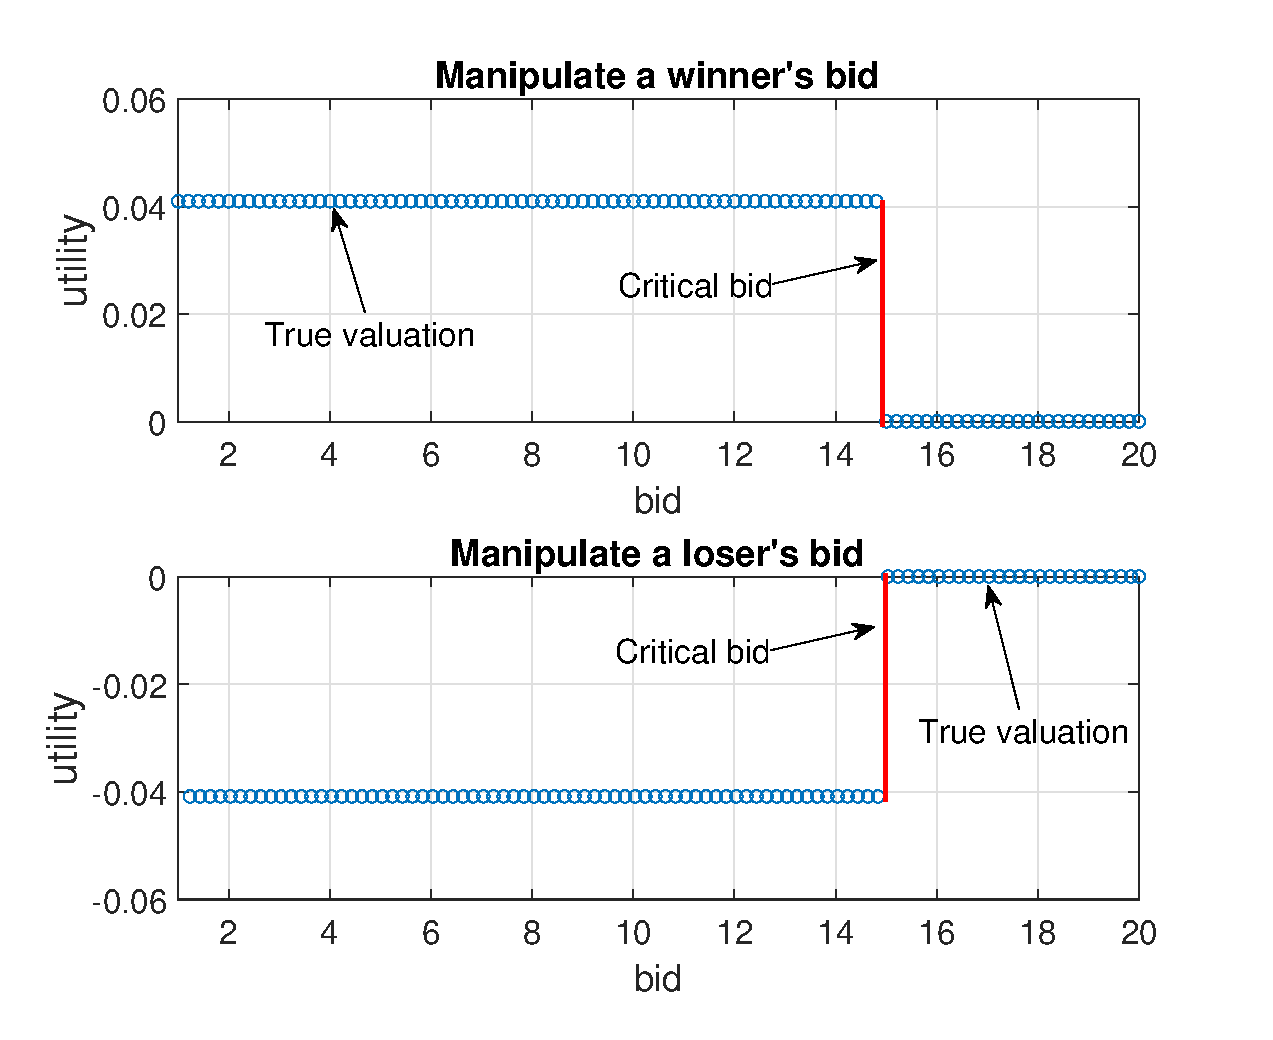
\includegraphics[scale=0.34]{./pic/truthfulness.eps}
%		\vspace{-0.2cm}
%		\caption{Truthfulness of the DPDA algorithm.}\label{fg:truthfulness}
%		\vspace{-0.0cm}
%	\end{figure}

\noindent{\textbf{计算复杂度}}
图\ref{fg:complexity}展示了算法DPDA的计算复杂度。对于$N$的每个取值,我们运行100次实验来评估算法的平均运行时间。实验中参数按节\ref{sec:setup}所述随机生成。我们实验所使用的PC配备有2.7GHz Intel Core i7处理器和16GB RAM。在不同的设置(即不同的失真度级别,出价和用户权重)下,我们观察到提出的DPDA算法的计算时间很短,并且与问题大小近似成线性关系。
%In Fig. \ref{fg:complexity}, we illustrate the computational complexity of the proposed DPDA algorithm. For each $N$, we examine the average running time of the algorithm by running 100 experiments, in which the parameters are randomly generated as mentioned in Section \ref{sec:setup}. These experiments are run on a PC with a 2.7 GHz Intel Core i7 processor and 16 GB RAM. Under different settings (i.e., different distortion levels, bids, and weights), we observe that the computation time of the proposed DPDA algorithm is low and approximately linear with the problem size.

	\begin{figure}[h!]
		\vspace{-0.2cm}
		\centering
		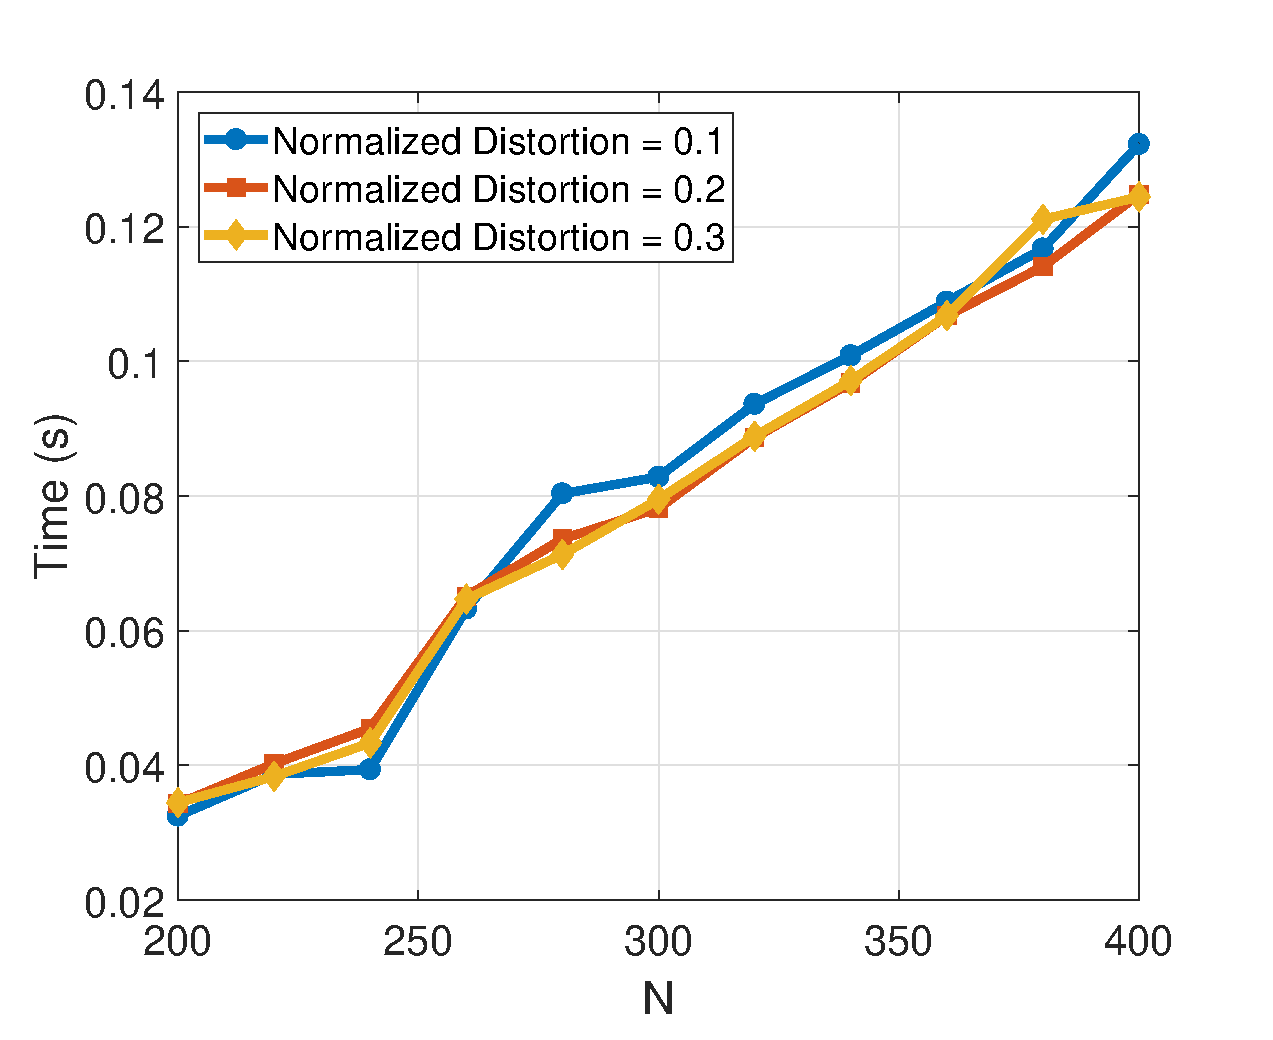
\includegraphics[scale=0.52]{./pic/complexity.eps}
		\vspace{-0.2cm}
		\caption{不同参数设置下DPDA的运算耗时。}\label{fg:complexity}
		\vspace{-0.3cm}
	\end{figure}

\section{本章小结}\label{sec:toncon}
本章在拍卖机制的框架下研究了隐私保护下的移动群智感知数据聚合问题,其中群智感知平台作为拍卖者征召移动用户来完成感知任务。在此模型下,本章应用差分隐私的概念设计了一种新颖的移动群智感知系统。具体来说,本章第2节提出了一种允许每个用户报告带有噪声数据的数据聚合方案,其中用户所允许添加的噪声分布由感知平台决定,使得用户的数据隐私保护程度可以通过差分隐私的量化指标进行衡量。本章第3节进一步提出了一个具有诚实性、个体合理性,且计算效率高的激励机制(DPDA)。该机制可以寻找到一组用户,在聚合结果准确性约束下,近似地将征召移动用户所需的成本降至最低。进一步,本章第4节将第3节提出的消极隐私保护框架泛化到一种积极隐私保护的场景。在这种场景中,用户可以通过竞标最低可接受的隐私保护级别来更好地控制其数据隐私保护级别。通过理论分析和充分的数值仿真,本文验证了DPDA算法和EDPDA算法的性能。
%We studied privacy-preserving data aggregation for mobile crowdsensing in an auction framework, where the platform plays the role as an auctioneer to recruit workers to complete a sensing task. Under this model, we designed a novel mobile crowdsensing system by leveraging the concept of differential privacy. Specifically, we designed a data aggregation that allows each worker to report a noisy data and can guarantee the use of each worker's data in a differentially private manner. Then, we designed a truthful, individual rational and computationally efficient incentive mechanism that can find a set of workers to approximately minimize the cost of purchasing the private sensing data from workers subject to the accuracy requirement of the aggregated result. We then generalize our results to a privacy-proactive scenario where workers could gain more control of their perceived data privacy protection level by beginning with bidding the lowest acceptable privacy level. We validated the performance of our proposed DPDA algorithm and EDPDA algorithm for the two scenarios through theoretical analysis as well as extensive simulations. 

